%%%%%%%%%%%%%%%%%%%%%%%%%%%%%%%%%%%%%%%%%%%%%%%%%%%%%%%%%%%%%%%%%%%%
%% I, the copyright holder of this work, release this work into the
%% public domain. This applies worldwide. In some countries this may
%% not be legally possible; if so: I grant anyone the right to use
%% this work for any purpose, without any conditions, unless such
%% conditions are required by law.
%%%%%%%%%%%%%%%%%%%%%%%%%%%%%%%%%%%%%%%%%%%%%%%%%%%%%%%%%%%%%%%%%%%%

\documentclass[
  color, %% This option enables colorful typesetting. Replace with
         %% `monochrome`, if you are going to print the thesis on
         %% a monochromatic printer.
  table, %% Causes the coloring of tables. Replace with `notable`
         %% to restore plain tables.
  lof,   %% Prints the List of Figures. Replace with `nolof` to
         %% hide the List of Figures.
  lot,   %% Prints the List of Tables. Replace with `nolot` to
         %% hide the List of Tables.
  %% More options are listed in the class documentation at
  %% <http://mirrors.ctan.org/macros/latex/contrib/fithesis/fithesis/guide/mu/fi.pdf>.
]{fithesis3}
%% The following section sets up the locales used in the thesis.
\usepackage[resetfonts]{cmap} %% We need to load the T2A font encoding
\usepackage[T1,T2A]{fontenc}  %% to use the Cyrillic fonts with Russian texts.

\usepackage[
  main=english, %% By using `czech` or `slovak` as the main locale
                %% instead of `english`, you can typeset the thesis
                %% in either Czech or Slovak, respectively.
  german, russian, czech, slovak %% The additional keys allow
]{babel}        %% foreign texts to be typeset as follows:
%%
%%   \begin{otherlanguage}{german}  ... \end{otherlanguage}
%%   \begin{otherlanguage}{russian} ... \end{otherlanguage}
%%   \begin{otherlanguage}{czech}   ... \end{otherlanguage}
%%   \begin{otherlanguage}{slovak}  ... \end{otherlanguage}
%%
%% For non-Latin scripts, it may be necessary to load additional
%% fonts:
\usepackage{paratype}
\def\textrussian#1{{\usefont{T2A}{PTSerif-TLF}{m}{rm}#1}}
\usepackage{xcolor} 
\newcommand{\todo}[1]{\textcolor{red}{\textbf{#1}}}
\usepackage{listings}
\usepackage[binary-units=true]{siunitx}
%%
%% The following section sets up the metadata of the thesis.
\thesissetup{
    university    = mu,
    faculty       = fi,
    type          = bc,
    author        = Samuel Petrovič,
    gender        = m,
    advisor       = Adam Rambousek,
    title         = {The effects of age \\ on file system performance},
    TeXtitle      = {The effects of age \\ on file system performance},
    keywords      = {file system, performance, aging, benchmarking, fragmentation, storage, trim, fs-drift, XFS, ext4},
    TeXkeywords   = {file system, performance, aging, benchmarking, fragmentation, storage, trim, fs-drift, XFS, ext4},
assignment = {}
}
\thesislong{abstract}{
The purpose of this thesis is to research effects of age on file system performance. For the testing purpose, two automated tests were implemented, which use open source benchmarks fs-drift and FIO to simulate aging and to measure performance. Research was aimed at effects of aging on popular Linux file systems, XFS and ext4. Further research examined effects of underlying storage technology on performance of aged file systems. Implemented file system aging test was used to expand testing matrix of Red Hat Kernel Performance team.
}
\thesislong{thanks}{
I would like to thank my consultant Matúš Kocka for tremendous help and guidance during writing of this thesis. I would also like to thank Red Hat for collaboration and provision of necessary testing equipment. 
}
%% The following section sets up the bibliography.


\usepackage{csquotes}
\usepackage[              %% When typesetting the bibliography, the
  backend=bibtex,          %% `numeric` style will be used for the
  style=numeric,          %% entries and the `numeric-comp` style
  citestyle=numeric-comp, %% for the references to the entries. The
  sorting=none,           %% entries will be sorted in cite order.
  sortlocale=auto         %% For more unformation about the available
]{biblatex}               %% `style`s and `citestyles`, see:
%% <http://mirrors.ctan.org/macros/latex/contrib/biblatex/doc/biblatex.pdf>.
\addbibresource{citations2.bib} %% The bibliograpic database within

                          %% the file `example.bib` will be used.
\usepackage{makeidx}      %% The `makeidx` package contains
\makeindex                %% helper commands for index typesetting.
%% These additional packages are used within the document:
\usepackage{paralist}
\usepackage{amsmath}
\usepackage{amsthm}
\usepackage{amsfonts}
\usepackage{url}
\usepackage{menukeys}
\usepackage{pdfpages}
\usepackage{mwe}

\renewcommand{\lstlistingname}{Example}
\renewcommand{\lstlistlistingname}{List of \lstlistingname s}



\begin{document}
\chapter{Introduction}
File systems remain an important part of modern storage solutions. Large, growing databases, multimedia and other storage based applications need to be supported by high-performing infrastructure layer of storing and retrieving information. Such infrastructure have to be provided by the operating systems (OS) in a form of file system.

Originally, file system was a simple tool developed to handle communication between OS and physical device, but today, it is a very complex piece of software with a large set of tools and features to go~with.

Performance testing is an integral part of development cycle of most of produced software. Because of growing complexity of file systems, performance testing took of as an important part of file system evaluation.

The standard workflow of performance testing is called \emph{out-of-box testing}. Its principle is to run benchmark (i.e. testing tool) on a clean instance of OS and on a clean instance of tested file system~\cite{Traeger:2008:NYS:1367829.1367831}. Generally, this workflow presents stable and meaningful results, yet it only gives overall idea of file system behavior in early stage of its life cycle. 

File systems, as well as other complex software, are subjected to progressive degradation, referred to as software aging~\cite{Cotroneo:2014:SSA:2543749.2539117}. Causes of file system aging are many, but mostly fragmentation of free and used space and unclustered data~\cite{Smith:1997:FSA:258623.258689}. This degradation cause problems in performance and functionality over time. Understanding of performance changes of aged file system can help developers to implement various preventions of aging related problems. Furthermore, aging testing can help developers with implementation of long-term performance affecting features.

Researching of file system aging can by done in two stages, aging the file system and testing of the aged instance. In the first stage, observation about \emph{evolution} of fragmentation and performance can be made. The second stage brings insight into \emph{state} of performance of aged file system.

In the first part, this thesis describes implementation of two flexible tests, which correspond with aforementioned stages.
 
In the first-stage testing, file system is aged using open-source benchmark fs-drift. While aging the file system, fragmentation of free space and latency of IO operations is periodically recorded. After the aging process, additional information about file systems block layout is recorded as well. Once this information is gathered, image of aged file system instance is created. To save space, only metadata of created file system is used, since content of created files is random and therefore irrelevant.

Created images are then used in second-stage testing. By using created images, higher stability and consistency of results is achieved. By reloading the file system image on the device, it is possible to bring the file system to the original, aged, state therefore for every performance test the same file system layout is available.

In the second-stage testing, file system is brought to the aged state by reloading image corresponding with desired testing configuration. Before every performance test, some volume can be released from file system, so the performance test has space to test on. After environment initialization (\texttt{sync}, \texttt{fstrim}), the performance test can begin. Testing of fresh instance of file system is done as well to conclude if any performance change occur.

In the latter parts of this thesis, usage of developed tests on different configurations of file systems and storage is demonstrated. The subject of research is difference between popular Linux file systems (XFS, ext4) and differences between used storage technologies (solid state and hard disk drives) in context of aging. Because of nature of collected data, a processing tool was implemented to parse large amount of information into human readable reports with interactive charts.\footnotemark[1]

\footnotetext[1]{Charts were created using JavaScript charting library Highcharts.~\cite{highcharts}}

In the Chapter~\ref{related}, the text presents already conducted research of effects of age and fragmentation on file system performance. Chapter~\ref{fs} describes used storage and file systems and their main features. Chapter~\ref{tools} introduces tools used in implementation of tests while describing their relevant features. Chapters~\ref{aging} and~\ref{fio} describe implementation of mentioned tests. Chapter~\ref{results} describes testing environment, means of data evaluation and results obtained by using created tests. The research is focused on describing the effects of file system aging, differences between file systems in terms of aging and relations of underlying storage to performance of aged file system. In~Chapter~\ref{conclusion}, I discuss results achieved by this thesis. Furthermore, future of testing of file system performance and aging is discussed.

Appendix~\ref{reports} contains all charts generated by automated reporting tool implemented for purpose of this thesis. Appendix~\ref{examples} contains examples of usage of implemented tests in Beaker environment and other examples of Beaker environment usage. Appendix~\ref{source} describes files attached as electronic appendix.

\chapter{Related work}
\label{related}
In this chapter I present different approaches of file system aging and fragmentation research described and implemented in the past. The first section discuss usage of collected data to create aging workload. The second section discuss possibilities of aging the file system artificially, without pre-collected data.

\section{Aging file system using real-life data}
This approach is based on modeling the aged file system using data collected from file systems used in real-life environment.

Such data can be in form of snapshots (i.e. images) of file systems, as was thoroughly described by Smith and Seltzer~\cite{Smith:1997:FSA:258623.258689}.

The snapshots were collected nightly over a long period of time (one to three years) on more then fifty file systems. By comparing pairs of snapshots in the sequence, performed operations were estimated, resulting in a very realistic aging workload. However, as some studies suggest, most of the files have life span shorter than 24 hours~\cite{Ousterhout:1985:TAU:323647.323631}. Therefore, as Smith and Seltzer admit, by snapshoting every night, this process does not account for most of the created files, resulting in loss of important part of data.

Furthermore, to age a file system sized $\SI{1024}{\mega\byte}$, $\SI{87.3}{\giga\byte}$ of data had to be written, taking 39 hours to complete, rendering the workflow impractical for in-production testing needs.

%Smith and Seltzer also defined a layout score as a method to evaluate fragmentation of a file system. Layout score is defined as a fraction of blocks of file, which are contiguously allocated. Files of one block size are ignored, since they can't be fragmented, and for every file, first block is ignored too. Evaluation of the whole file system is then computed as an aggregated layout score of all files.

The problem resulting from not tracking shortly lived files can be solved by another approach called collecting traces. Traces are sequences of IO operations performed by OS, captured at various levels (system calls, drivers, network, etc.). The sequence of operations can be replayed back to the file system, aging it in a realistic manner.

Overall, using real-life data to age file systems brings realistic results, but at a cost of higher expenses, such as storing the collected data. Additionally, to cover cases of different types of file system usage, data from several such file systems have to be collected, expanding the amount of needed data even further. Such materials are not always available, rendering this type of approach useful only in cases the researcher is already in their possession.

\section{Synthetic aging simulation}
Synthetic aging is a type of aging that does not require real-life data for its running. It relies on purely artificial workload performed on a file system, invoking aging factors, such as fragmentation.

Fast file system aging was described as a part of a trace replay benchmark called TBBT~\cite{Zhu:2005:TSA:1251028.1251052}. This type of aging consists of sequence of interleaving append operations on a set of files. By controlling the amount of files involved in the process, researchers had great control over final fragmentation. Such workflow, while creating desired fragmentation, is however quite unrealistic, making the results of testing on such file system questionable~\cite{Traeger:2008:NYS:1367829.1367831}.

Another attempt of inducing fragmentation was made in an empirical study of file system fragmentation in mobile storage systems~\cite{ji2016empirical}. The aging process consisted of filling the device by alternative creation of files larger or equal to $\SI{100}{\mega\byte}$ and smaller or equal to $\SI{100}{\kilo\byte}$. After 100\% file system utilization was reached, 5\% of files was randomly deleted. 

However, for truly realistic insight, a workflow generator which tries to mimic real-life usage can be more suitable.

A workload generator such as fs-drift\footnotemark[1], can be used (while carefully configured) to simulate desired long term real-life usage. While running, fs-drift is creating requests of variety of IO operations. The probability with which would be operation chosen can be controlled by workload table. In addition, this tool offers different probability distributions of file access, making it easier to mimic behavior of natural user. Furthermore, whole process is highly configurable, making it possible to simulate various types of file system usage. Such qualities predispose fs-drift to be capable of achieving more realistic results then previous attempts.

\footnotetext[1]{Mixed workload file system aging test~\cite{fs-drift:github}.}

\chapter{File system and storage devices}
\label{fs}
In this chapter, I present basic information about used file systems, storage devices and its features relevant to performance and aging.

\section{File systems}
File system is a set of tools, methods, logic and structure to control how to store and retrieve data on and from device.

The system stores files either continuously or scattered across device. The basic accessed data unit is called a block, which capacity can be set to various sizes. Blocks are labeled as either free or used.

Files which are non-contiguous are stored in form of extents, which is one or more blocks associated with the file, but stored elsewhere.  

Information about how many blocks does a file occupy, as well as other information like date of creation, date of last access or access permissions is known as metadata, i.e. data about stored data. This information is stored separately from the content of files. On modern file systems, metadata are stored in objects called index nodes (i.e. inodes). Each file a file system manages is associated with an inode and every inode has its number in an inode table. On top of that the file system stores metadata about itself (unrelated to any specific file), such as information about bad sectors, free space or block availability in a structure called superblock.

In this thesis, targeted file systems are two popular Linux file systems~\cite{Lu:2013:SLF:2591272.2591276}, XFS\footnotemark[1] and ext4\footnotemark[2]. These file systems belong to a category of journaling file systems.

Journaling file system keeps a structure called journal, which is a buffer of changes not yet commited to the file system. After system failure, these planned changes can be easily read from the journal, thus making the file system easily fully operational, and in a correct and consistent state~\cite{prabhakaran2005analysis}.

\footnotetext[1]{XFS file system~\cite{xfs:qhe}.}
\footnotetext[2]{Fourth extended file system~\cite{ext4:qhe}.}

\subsection{XFS}
XFS is a 64-bit journaling file system known for its high scalability (up to $\SI{9}{\exa\byte}$) and great performance. Such performance is reached by architecture based on allocation groups.

Allocation groups are equally sized linear regions within the file system. Each allocation group manages its own inodes and free space, therefore increasing parallelism. Architecture of this design enables for significant scalability of bandwidth, threading, and size of file system, as well as files, simply because multiple processes and threads can access the file system simultaneously.

XFS allocates space as extents stored in pairs of $B^+$ trees, each pair for each allocation group (improving performance especially when handling large files). One of the $B^+$ trees is indexed by the length of the free extents, while the other is indexed by the starting block of the free extents. This dual indexing scheme allows efficient location of free extents for IO operations.

Prevention of file system fragmentation consist mainly of features called delayed allocation and online defragmentation.

Delayed allocation, also called allocate-on-flush, is a feature that, when a file is written to the buffer cache, subtracts space from the free space counter, but won't allocate the free space bitmap. The data is held in memory until it have to be stored because of system call. This approach improves the chance the file will be written in a contiguous group of blocks, avoiding fragmentation and reducing CPU usage as well.

\subsection{Ext4}
Ext4, also called fourth extended file system is a 48-bit journaling file system developed as successor of ext3 for Linux kernel, improving reliability and performance features. ext4 is scalable up to $\SI{1}{\exbi\byte}$ (approximately $\SI{1.15}{\exa\byte}$). Traditional ext2 and ext3 block mapping scheme was replaced by extent based approach similar to XFS, which positively affects performance.

Similarly to XFS, ext4 use delayed allocation to increase performance and reduce fragmentation. For cases of fragmentation that still occur, ext4 provide tool for online defragmentation \texttt{e4defrag} to defragment either single file, or whole file system. Performance penalties were, however, recognized and extended online defragmentation workflow was proposed by Sato~\cite{sato2007:ext4}.


%Ext4 provide support for online defragmentation~\cite{sato2007:ext4} and \textit{e4defrag} tool to defragment either single file, or whole file system.


\section{Storage}
\subsection{Hard disk drive}
A hard disk drive (i.e. HDD) is a type of storage device which use one or more magnetic plates to store data. Data can be retrieved by rotating the plates and positioning magnetic read-write heads. The plates rotate at stable speed at around 7500\,rpm (and more in enterprise level hardware).

Since the parts of HDD have to physically move to reach desired location, there is a latency to the data access. The time for magnetic head to find next relevant block of data is called a \emph{seek time}. Because the length of seek time has significant impact on overall IO performance, OS have to do a lot of optimising, such as pre-fetching.

Obviously, block layout would have a large impact on performance of this kind of device. The amount of fragmentation (thus aging) affect the number of performed seeks. This cause the pressure on file system to store data more contiguously and also cluster related data.

\subsection{Solid state drive}
Solid state drive (i.e. SSD) is  a type of storage device which use integrated circuit to store and retrieve data. SSD has no moving parts, therefore the data access is purely electronic, which results in lower access time and latency than HDD~\cite{kasavajhala2011solid}.

However, on SSD, data cannot be directly overwritten (as in HDD). The cell of an SSD can only be directly written to, therefore have to be erased before writing. Moreover, due to physical construction limits, write operation can be conducted on one page (4-$\SI{16}{\kilo\byte}$), but erasure have to be done on a whole block (128 to 512 pages)~\cite{Hu:2009:WAA:1534530.1534544}. Therefore, if OS have to rewrite some part of a page (e.g. update metadata), the page have to be read, modified and submitted back on available part of the drive. The original page is then marked as discarded. This effect is known as write amplification and is computed as amount of bytes written to the device divided by amount of bytes requested to be written by user~\cite{Hu:2009:WAA:1534530.1534544}. For example, if user updates $\SI{512}{\byte}$ of data on device that uses $\SI{8}{\kilo\byte}$ pages, write amplification is then 16.

In addition, the memory cell can be rewritten finite amount of times, therefore a form of wear leveling has to be employed. Wear leveling prevents frequently accessed blocks from exhaustion of cell life-cycle by moving files around the device.

Static wear leveling rotates even unused files around the drive to ensure equal wear~\cite{Chang:2007:EEF:1278480.1278533}. However, deleting file, in file system doesn't always ensure its deletion on the device. Typically, the file is only marked as deleted, but this information is not submitted to underlying device itself. The problem is, the files which are not valid for file system anymore can still circulate on the device, increasing its wear and write amplification, since there is lower amount of available pages to write to.

To decrease this effect, trim commands were introduced~\cite{Frankie:2012:MMT:2184512.2184527}. Trim command communicate to SSD all the deletions that were realised in the file system, so the drive can erase blocks accordingly. Nevertheless this operation is reducing performance of IO operations while being conducted, it can increase overall performance and life time of an SSD.



\chapter{Environment setup and benchmark tools}
\label{tools}
In this chapter, I present tools which were used to implement automated tests for creating and storing aged file systems and measuring their performance. Furthermore, I describe the main features and means of their usage. All the presented tools are open source projects.

\section{Beaker}
Beaker is an open source Red Hat community project aimed at automating testing workflow~\cite{beaker}. The software can provision system from a pool of labs, install OS and packages, configure environment and perform tasks. The whole process is guided by sequence of instructions in an XML format. Examples of usage can be found in the Appendix~\ref{examples}.

\section{Storage generator}
Storage generator is a Beaker task developed by Jozef Mikovič as an internal Red Hat tool. It is capable of automated configuration of storage on a provisioned system. In a single device mode, storage generator simply creates new partition on the given device and creates and mounts file system. In a recipe mode, storage generator follows set of instruction to create more advanced configurations such as merging multiple devices using LVM, creating LVM cache or encrypted volume. Example of usage can be found in Example~\ref{ex:storage_generator}.

The creation of XFS file system is standard, but ext4 file system is created with an additional option, disabling \emph{lazy init}. Lazy init is a feature which allows for fast creation of file system by not allocating all the available space at once. The space is allocated later, as the file system grows. Such additional allocation, however would skew data collected in the first hours of the test, therefore it is disabled in these tests.

\section{FIO}
Flexible Input/Output benchmark is a workload generator written by Jens Axboe~\cite{fio:github}. It is a tool well known for it's flexibility as well as large group of users and contributors. The flexibility is integral for conducting less artificial and more natural performance tests. However, approaching more natural test behavior, stability of results drop, so ideal equilibrium between these two requirements has to be found.

FIO accepts the workload specification as either a configuration file or a single line. Multiple different jobs can be specified as well as global options valid for every job. 

There is a possibility to choose from variety of IO operations to be performed. Verification of the issued data is offered as well. Size of generated file and block size can be controlled too and it can be either stable or chosen from given range. For cache-tiering workloads, different random distributions (e.g. Zipf, Gauss) can be specified. FIO also supports process forking and threading.

After the test, FIO generates overall report of measured performance. Logging of multiple properties can be enabled, giving researchers even more oversight about the nature of file system performance.

\section{Fs-drift}
Fs-drift is a very flexible aging test, which can be used to simulate lots of different workloads~\cite{fs-drift:github}. The test is based on random file access and randomly generated mix of requests. These requests can be writes, reads, creates, appends, truncates, renames and creations of hard and soft links.

At the beginning of run time, the top directory is empty, therefore create requests success the most, other requests, such as \texttt{read} or \texttt{delete}, will fail because not many files has yet been created. Over time, as the file system grows, create requests began to fail and other requests will more likely succeed. File system will eventually reach a state of equilibrium, when requests are equally likely to execute. From this point, the file system would not grow anymore, and the test runs unless one of the stop conditions is met.

The mix of operation probabilities can be specified in separate CSV file. Fs-drift will try to issue more create operations at the beginning of testing, so other operations execute with higher likeliness.

The file to perform a request on is randomly chosen from the list of indexes. If the type of random distribution is set to \emph{uniform}, all indexes have the same probability to be chosen. If the type of random distribution is set to \emph{gaussian}, the probability will behave according to normal distribution with the center at index 0 and width controlled by parameter \texttt{gaussian-stddev}. This is useful for performing cache-tiering tests. File index is computed as modulo maximal number of files, therefore instead of accessing negative index values, the test access indexes from the other side of the spectrum, see Figure~\ref{fig:rand2}

Furthermore, fs-drift offers another option to influence random distribution. After setting parameter \texttt{mean-velocity}, fs-drift will choose files by means of moving random distribution. The principle relies on a simulated time, which runs inside the test. For every tick of the simulated time, the center of bell curve will move on the file index array by the value specified by \texttt{mean-velocity} parameter. By enabling this feature, the process of testing moves closer to reality by simulating more natural patterns of file system access (the user won't access file system randomly, but rather works with some set of data at a time). On Figure \ref{fig:rand3}, you can see bell curve moving by 5 units two times.

\begin{figure}[!htb]
%    \centering
%   \begin{minipage}{\textwidth}
%        \centering
%        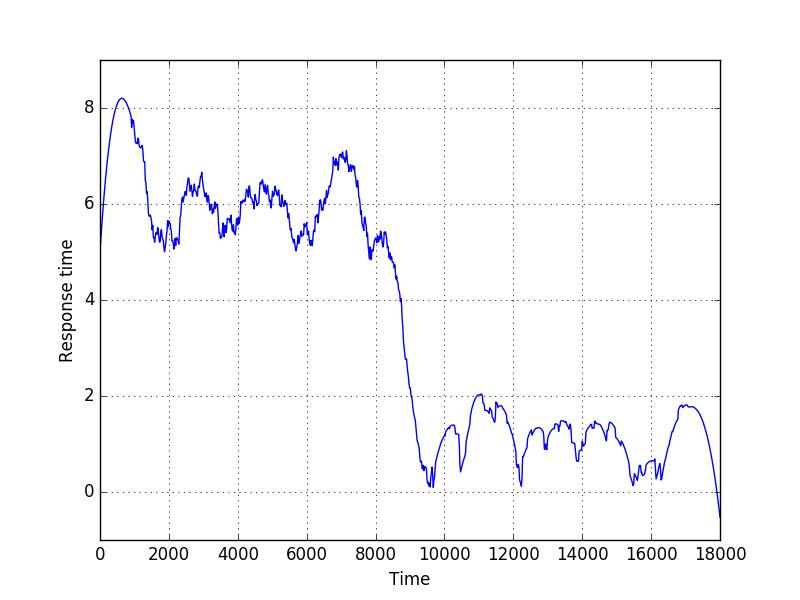
\includegraphics[width=0.7\textwidth]{../scripts/fig1.png}
%        \caption{Uniform distribution of file access}
%\label{fig:rand1}
%    \end{minipage}\hfill
    \begin{minipage}{\textwidth}
        \centering
        \includegraphics[width=0.7\textwidth]{../scripts/fig2.png}
        \caption{Normal distribution of file access}

\label{fig:rand2}
    \end{minipage}

\end{figure}
\begin{figure}
    \begin{minipage}{\textwidth}
        \centering
        \includegraphics[width=0.7\textwidth]{../scripts/fig3.png}
        \caption{Moving random distribution}
\label{fig:rand3}
    \end{minipage}
\end{figure}

%For purpose of this thesis, several changes had to be made to the original code. Besides small errors like invalid Readme information, a bug in code had to be repaired, otherwise the fs-drift would not delete files while issuing \textit{delete} operation, marginally affecting aging process. Without this fix, the volume would just saturate and remain in more or less consistent state for the rest of the runtime.

%Additionally, to be able to inspect and work with the file system while aging process is still running, I added an option to specify \textit{pause file}. If the pause file is present, the fs-drift would not issue any requests and waits until the file is removed\footnotemark[1].
%\footnotetext[1]{For all the changes made to master branch of fs-drift, see ...}

Fs-drift offers even more parameters to control the test run such as number of directories, number of levels of directories or enabling \texttt{fsync}/\texttt{fdatasync} to be called. To stop the fs-drift, one of the stop conditions have to be met. The stop condition can be either reached maximal number of performed operations, running out of time, or appearance of stop file.

For evaluation of the aging process, fs-drift can log latency of the performed operations. However, the log doesn't differentiate between the operations, which could be useful for further research.

Used configuration of fs-drift for purposes of aging testing is further described in Chapter~\ref{aging}.

\subsection{Changes in original code}
\label{text:fsdrift_changes}
Several changes had to be made in the original code prior to testing.

The most obvious problem with the tools was, that it did not conduct delete operations. Deleting files is important for inducing fragmentation, therefore, this error has to be repaired.

Another problem emerged with gathering  of statistics of latency evolution through the aging process. Since the tool is generating the IO requests at random, sometimes error occurs. Most operations need the file to exist to success, but sometimes, the file is non-existent. The problem with latency logging was that fs-drift logged the latency even if the operation didn't carry, causing noise in the data.

Further problem with latency logging was, it didn't differentiate between operations. Such distinction could greatly affect the way researchers can find problems with file system evolution.

As mentioned, possibility of specifying \emph{pause file} was added, making the fs-drift easy to pause when additional manipulation with file system is required.

Another feature added to fs-drift was non-uniform distribution of file sizes. Originally, fs-drift used only uniform distribution to choose file size from zero to specified maximum size. Such implementation offers very little control over file size distribution and is quite unrealistic. Therefore, possibility to request natural file size distribution was added. As a reference for file size distribution, five year old study of file system metadata was used~\cite{agrawal2007five}. Figure~\ref{fig:filedist} shows measured file size distribution of used file systems. To mimic this layout, log-normal distribution was modeled. The shape of resulting distribution is shown in Figure~\ref{fig:lognormal}.

The version used for testing in this thesis have all aforementioned features implemented and problems repaired.

\begin{figure}
    \centering
    \fbox{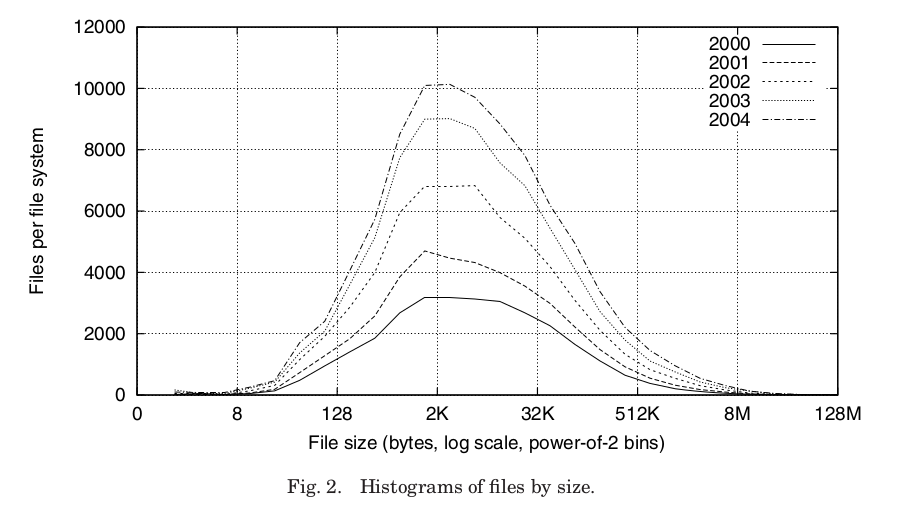
\includegraphics[width=\textwidth,keepaspectratio,trim=4 4 4 4,clip]{../charts/filedist.png}}
    \caption{File size distribution as measured by Agrawal.~\cite{agrawal2007five}}
    \label{fig:filedist}
\end{figure}

\begin{figure}%[!htb]
    \begin{minipage}{\textwidth}
        \centering
        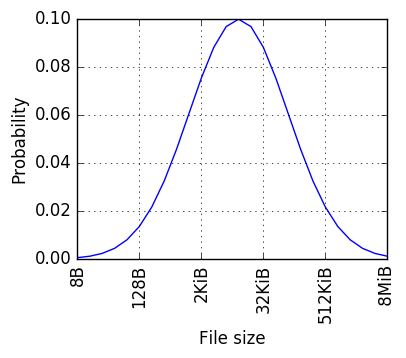
\includegraphics[width=0.7\textwidth]{../scripts/dist3.png}
        \caption{Log-normal distribution of file size.}
\label{fig:lognormal}
    \end{minipage}
\end{figure}



\chapter{Aging the file system}
\label{aging}
In this chapter, I describe process of development of file system aging workflow and its implementation as a form of automated test.

\section{Fs-drift configuration}
As mentioned, fs-drift was used as a means of bringing file systems to an aged, fragmented state. Fs-drift is quite flexible, therefore a lot of parameters and their impact on the final layout had to be considered.

First, the amount of fullness had to be taken into account. Heavily used file systems tend to be full at amounts ranging from~65\%~to~100\%~\cite{agrawal2007five,Smith:1997:FSA:258623.258689}. However, fs-drift does not offer an option to directly control the fullness of the file system. As the creator states in README, to fill a file system, maximum number of files and mean size of file should be defined such that the product is greater than the available space. Parameters to overload the volume are not difficult to come up with. The problem is, the random nature of the test doesn't allow for meaningful reproducibility of the reached equilibrium. In most cases, fs-drift plainly saturates given volume, so utilization remains at 100\% through the rest of the testing time. This drawback was overridden by a change in fs-drift code\footnotemark[1]. By adding the possibility to pause fs-drift, other processes can stop fs-drift to generate IO requests if the file system usage reaches a specified amount and release some space. This way, desired amount of maximal utilization can be reached.

\footnotetext[1]{For all the changes made in original code of fs-drift, see Chapter~\ref{tools}.}

%Duration of the test is an important factor as well. In general, the testing time should be long enough for the environment to stabilise. After developing a test, it is necessary to conduct few pilot runs to confirm if any stabilisation of performance occur and set the duration accordingly for best effectivity

% When considering file system aging, 


%the test should spend most of the run time after the saturation phase (e.g. the phase of filling the file system to a desired fullness). 



%. On the other hand, for the test to be useful in professional environment, testing time should not be too long. The goal is to maximize testing correctness while minimising the time for the test to complete. The ideal duration of testing is discussed and experimented with in Section~\ref{text:duration}

Fs-drift offers to control testing length by elapsed time. The elapsed time is computed as current time subtracted from starting time. However, pausing the fs-drift to release space, examine file system, etc. resulted in non-uniform testing time across runs. Therefore, testing length by operation count is used in conducted tests.

File size is another important factor of successful simulation. To consider a simulation successful, resulting layout should have similar file size distribution as real-life file systems. For that reasons natural file size distribution is used in all tests.\footnotemark[2] 

\footnotetext[2]{The specifics of natural file distribution are described in Chapter~\ref{tools}.}

During the test, more weight is placed on file system expanding operations (create, append, random write) to fill the file system faster. Non-altering operations are present to verify, if any performance drop occur during the aging process.

\section{File system images}
File system images can be created by using tools developed to inspect file systems in case of emergency. For Ext file systems, there is a tool called \texttt{e2image} and for XFS, \texttt{xfs\_metadump}. Both tools create images as sparse files, so compression is needed.

\texttt{E2image tool} can save whole contents of a file system or just its metadata and offers compression of image as well. Created images can be further compressed by tools such \texttt{bzip2} or \texttt{tar}. Such images can be later reloaded back on a device. From that point, file system can be mounted. Example~\ref{ex:e2image1} shows creating file system image using \texttt{e2image} tool. Example~\ref{ex:e2image2} shows reloading image on device.

\lstset{language=bash, 
numbers=none, 
frame=single, 
commentstyle=\color{dkgreen}, 
basicstyle={\scriptsize\ttfamily}, 
keywordstyle=\color{blue}, 
%identifierstyle=\color{blue}, 
stringstyle=\color{red},
captionpos=t,
showstringspaces=false,
breaklines=true,
breakatwhitespace=false,
tabsize=3,
caption={sdad},
}

\begin{lstlisting}[language=bash, label={ex:e2image1}, caption={Creating compressed image using \texttt{e2image}.}][frame=single]
  $ e2image -Q $DEVICE $NAME.qcow2
\end{lstlisting}

\begin{lstlisting}[language=bash, label={ex:e2image2}, caption={Reloading compressed image using \texttt{e2image}.}][frame=single]
  $ e2image -r $NAME.qcow2 $DEVICE
\end{lstlisting}

\texttt{Xfs\_metadump} saves XFS file system metadata to a file. Due to privacy reasons file names are obfuscated (this can be disabled by -o parameter). As well as \texttt{e2image} tool, the image file is sparse, but \texttt{xfs\_metadump} doesn't offer a way to compress the output. However, output can be redirected to standard output and compressed further on. Generated images, when uncompressed, can be reloaded back on device by tool \texttt{xfs\_mdrestore}. File system can be then mounted and inspected as needed. Example~\ref{ex:xfs_metadump} shows creating file system image using \texttt{xfs\_metadump}. Example~\ref{ex:xfs_mdrestore} shows reloading image on device using \texttt{xfs\_mdrestore}.

\begin{lstlisting}[language=bash, label={ex:xfs_metadump}, caption={Creating compressed image using \texttt{xfs\_metadump} and \texttt{bzip2}.}][frame=single]
  $ xfs_metadump -o $DEVICE -|bzip2 > $NAME
\end{lstlisting}

\begin{lstlisting}[language=bash, label={ex:xfs_mdrestore},caption={Reloading image using \texttt{xfs\_mdrestore}.}][frame=single]
  $ xfs_mdrestore $NAME $DEVICE
\end{lstlisting}

\section{Implementation details of file system aging test}
Workflow of image creating is contained in the Beaker task drift\_job. After extracting fs-drift, the main script (runtest.sh) starts Python script (run\_drift.py), which handles the process of running fs-drift. Settings of fs-drift are passed as a parameter and then parsed inside the script.

Before running the fs-drift, asynchronous thread \texttt{async\_worker} is triggered. \texttt{Async\_worker} offers ways to additionally control testing and to work with file system while the test is running. The thread wakes up at specified intervals. Upon awakening, fs-drift is paused, then free space fragmentation and file system usage is logged. If the usage reaches defined limit, specified amount of space is randomly released from file system. If the test runs on an SSD, \texttt{fstrim} can be optionally called. Furthermore, when all mentioned steps are completed, the thread calls \texttt{sync}, unpauses fs-drift and goes to sleep.

After fs-drift ends, fragmentation of used space is logged and image of file system is created using presented tools and archived using \texttt{bzip2}. All the generated data and information about environment is archived as well and a text file describing the test is generated. These three files are then sent (via \texttt{rsync}) to data collecting server.

For better oversight of the tests functionality, its activity diagram is presented in Figure~\ref{fig:drift_job_activity}. Example of execution of this task in Beaker environment can be found in Example~\ref{ex:age}. 
\clearpage
Parameters available for drift\_job:
\begin{compactenum}
  \item sync, flag to signalise weather or not to send data to server (useful for developing purposes)
  \item mountpoint
  \item disk, device used during test
  \item recipe, parameters to pass to fs-drift
  \item tag, string to distinguish different storage configurations
  \item drifttype, string to distinguish different aging configurations
  \item maintain, parameter to specify maximum volume usage and amount to be freed
  \item fstrim, parameter to specify if \texttt{fstrim} should be periodically called
  \end{compactenum}


\begin{figure}[ht]
    \centering
    \fbox{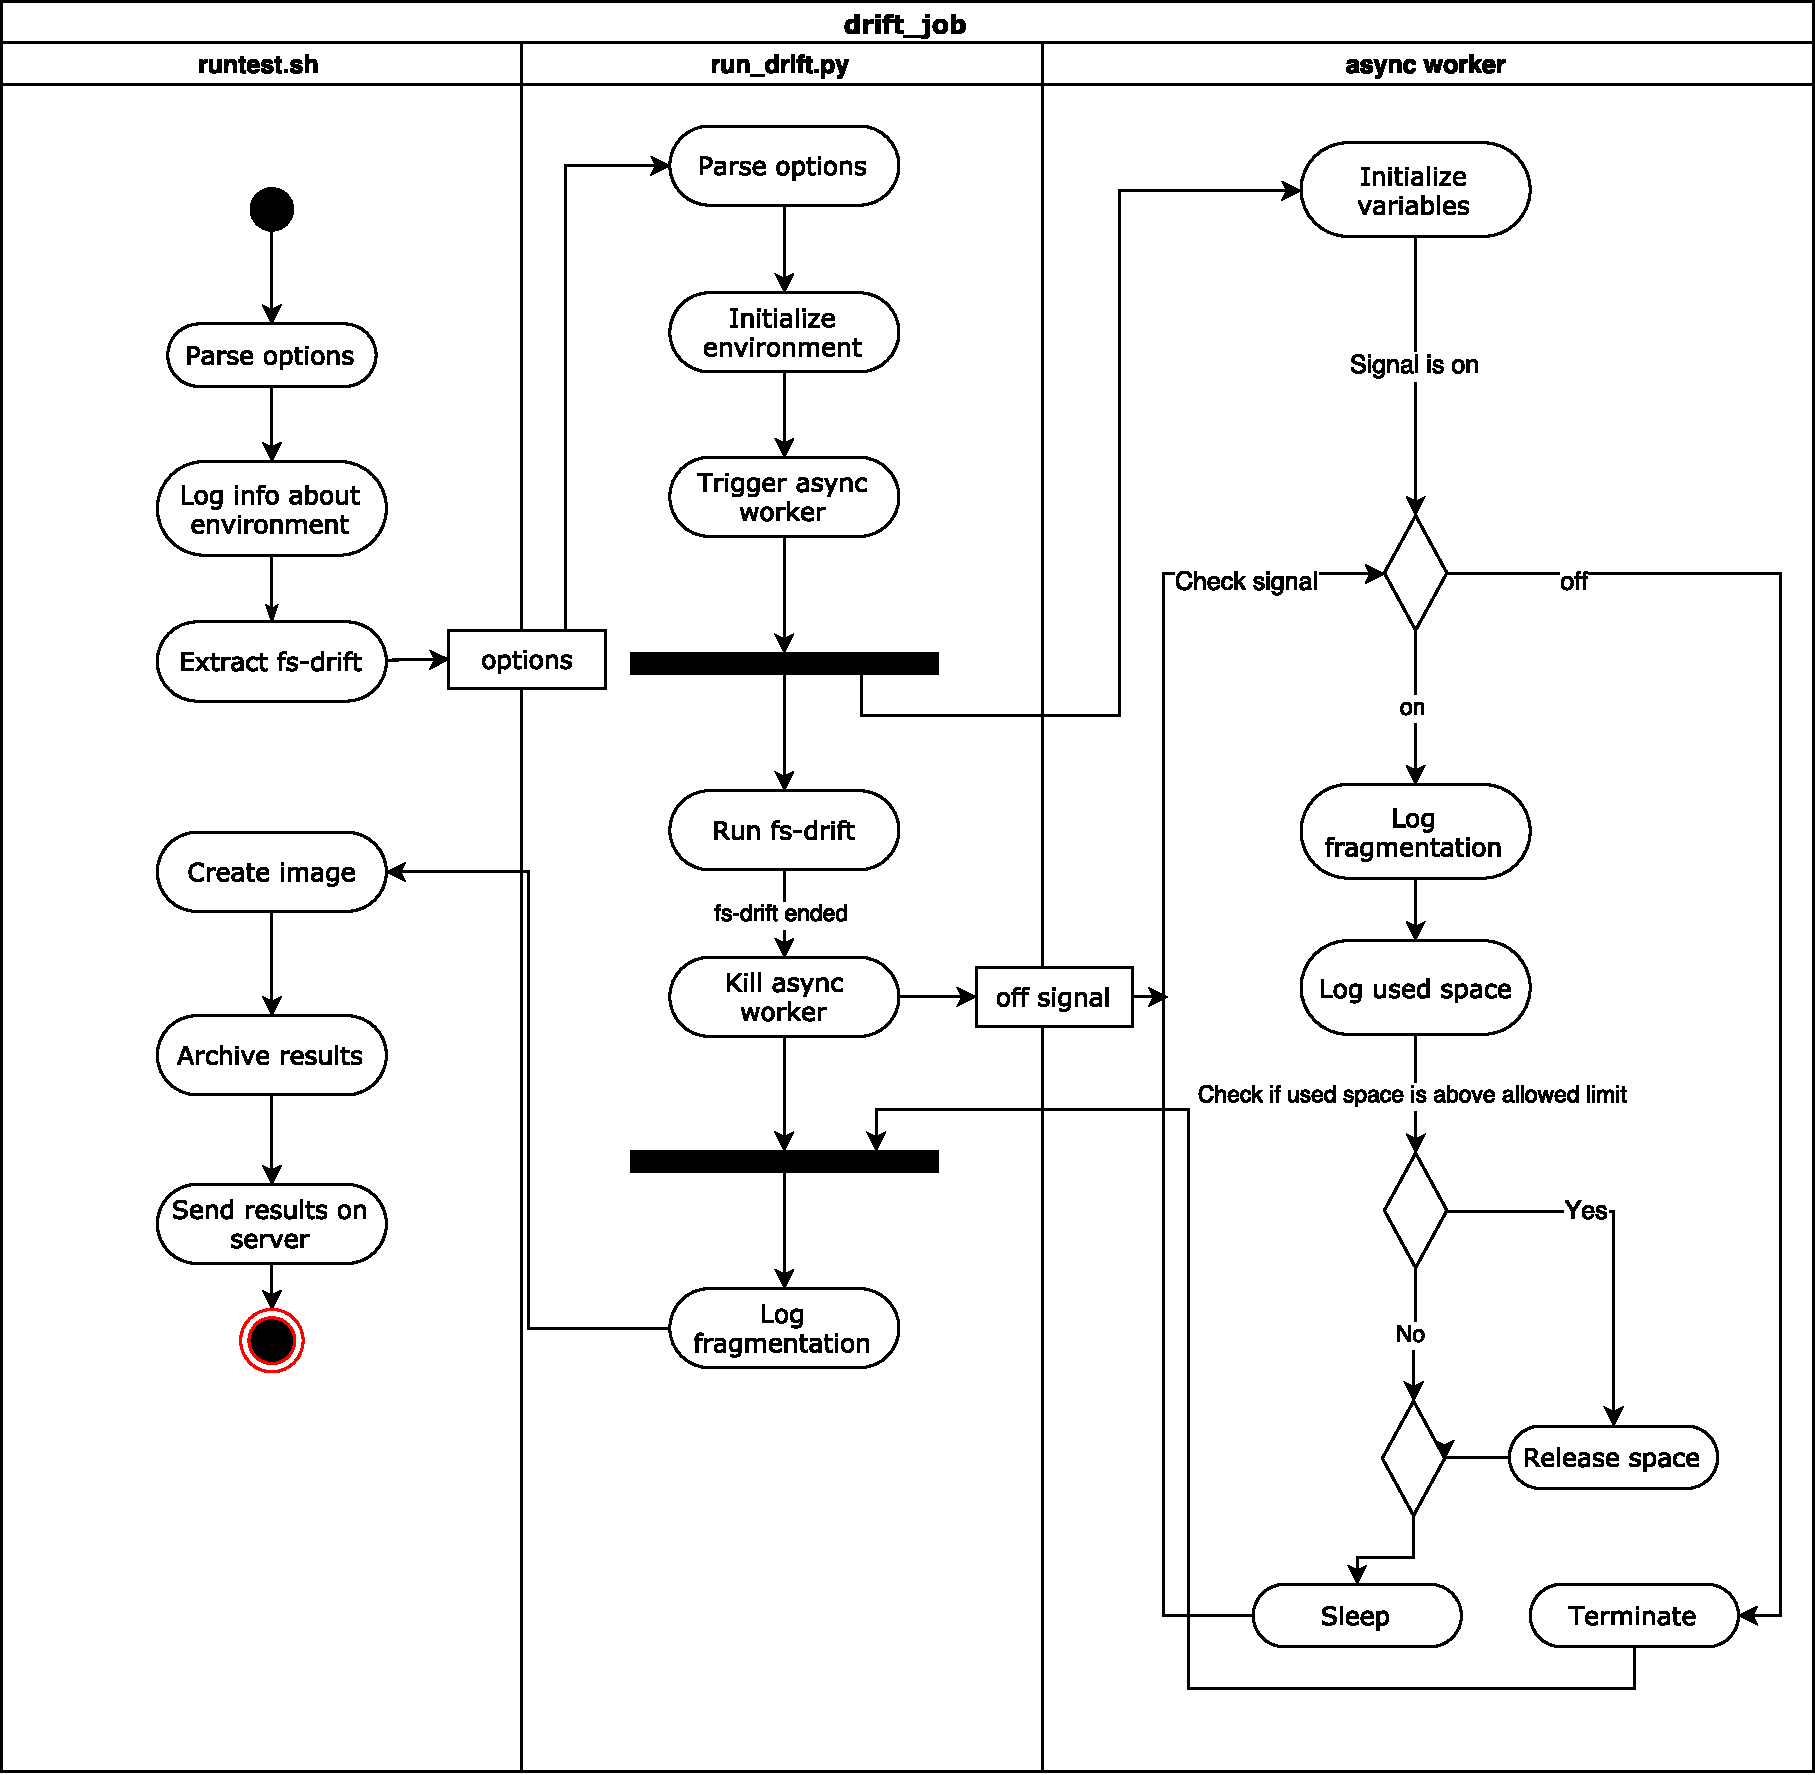
\includegraphics[width=\textwidth,keepaspectratio]{../scripts/drift_job_activity}}
    \caption{Activity diagram of file system aging test}
    \label{fig:drift_job_activity}
\end{figure}

\chapter{Performance testing of aged file system}
\label{fio}
In this chapter, I describe structure of performance test which use images created by aging test. In the first section, I present configuration of FIO benchmark and in second section, I describe implementation of testing workflow as an automated test.

\section{FIO configuration} 

%While designing FIO workload to test performance of aged file system, 

By default, FIO will create one file for every triggered thread. Furthermore, this file is created and opened before FIO begins issuing IO requests. This setting is unfit for file system aging testing, because the subject of interest is among others \emph{file allocation}.

The first step to make FIO workload more relevant to file system aging is to ask for creation of many files for every thread. The number of files was set in such a way, their individual size was approximately $\SI{4}{\kilo\byte}$. FIO will try to open all the files at once, which results in error for more than 102 files, therefore maximal amount of open files was specified to 100. Furthermore, to include creation of files and allocation into the performance measurement, \texttt{create\_on\_open} was set, so FIO creates file at the moment of opening, if the file does not exist. Another important factor is distribution of which FIO access the files. Default is set to round-robin, but was reset to gaussian, so the distribution of file access is more similar to file system aging test.

Similarly to aging test, FIO should perform \texttt{fsync} from time to time. This can be set as amount of write requests after which \texttt{fsync} should be performed.

Overall size is set in such a way, it consumes most of space left after loading the image. Same size is used while testing on fresh file system. Block size is set to $\SI{4}{\kilo\byte}$ as that is default block size of used file systems.

To ensure stable run time of FIO test, time-based testing is used with run time of 10 minutes. It is not expected of FIO to issue total specified size, but to measure the performance effectively.


%Volume is randomly removed using random\_delete\_volume.py script. This scriptt globs all files in the filesystem, retrieves information about used volume as well as it's overall size. Then proceeds to randomly choosing files to delete and stops when desired volume is freed. The approach of recursively globbing all files may be inefficient, but this way, we can be sure, that volume is deleted from whole device evenly.

%\section{Inspecting filesystem}

%To determine overall idea about an extent to which is the file system aged, scripts that generate histograms representing fragmentation of used space as well as fragmentation of free space. Both scripts use common linux tools and pyplot to generate the graphics. Both scripts can display linear or logarhytmic Y scale.

%Script extent\_distribution.py makes use of xfs\_io fiemap tool, which is a tool to display extent distribution of a given file and works correctly even for ext* filesystems.

%The script will first recursively crawls the whole filesystem from given top folder and makes a list of all files. Fiemap is then run over every file separately. 

%The only data, that are then parsed from the output, is how many non-contigous extents does the file have. These integers are aggregated to a single list, from which are then counted, and final histogram is made.

%Script free\_space\_fragmentation.py use the tool e2freefrag, which runs over a device, and outputs the histogram of free space fragmentation in texutal form. Script will store this output and then easily parse the histogram and aggregate the data into a graphic form.

\section{Implementation details of aged file system performance test}
Performance testing of created images is contained in Beaker task recipe\_fio\_aging. Upon installation of necessary tools (libraries, FIO), the package finds and downloads corresponding file system image according to obtained parameters. As shown, images are stored compressed, therefore decompression is needed after download. Once these steps are successfully completed, testing phase can begin.

Before every test, initialization is performed by running \texttt{sync}, \texttt{fstrim} and dropping caches.

At first, performance measurements of fresh a file system is done. Test configuration of fresh and aged test is similar, with an exception, that after testing fresh file system, FIO will delete all the created files. This is disabled for aged tests, because post-test fragmentation is gathered afterwards.

After testing fresh file system, image is loaded and mounted. If the mounted file system utilise too much space, some files can be randomly deleted. Afterwards, pre-test fragmentation is logged and environment is initalized. When the test is over, post-test fragmentation is gathered.

The configuration of FIO can be passed as parameter to recipe\_fio\_aging task. Such approach makes this testing workflow as flexible as original benchmark.

For statistical correctness, these tests can run in loops $n$ times. Fresh and aged testing is divided into separate loops.

After last iteration, the results are archived and sent to a data collecting server. 

For better oversight of the tests functionality, its activity diagram is presented in Figure~\ref{fig:rec_activity}. Example of execution of this task in Beaker environment can be found in Example~\ref{ex:fio}. 
\clearpage
Parameters available for recipe\_fio\_aging:
\begin{compactenum}
  \item sync, flag to signalise whether or not to send data to server (useful for developing purposes)
  \item numjobs, number of test repetitions. For statistical stability
  \item mountpoint
  \item device, device used during test
  \item recipe, parameters to pass to FIO
  \item tag, string to distinguish different tests
  \end{compactenum}

\begin{figure}[ht]
    \centering
    \fbox{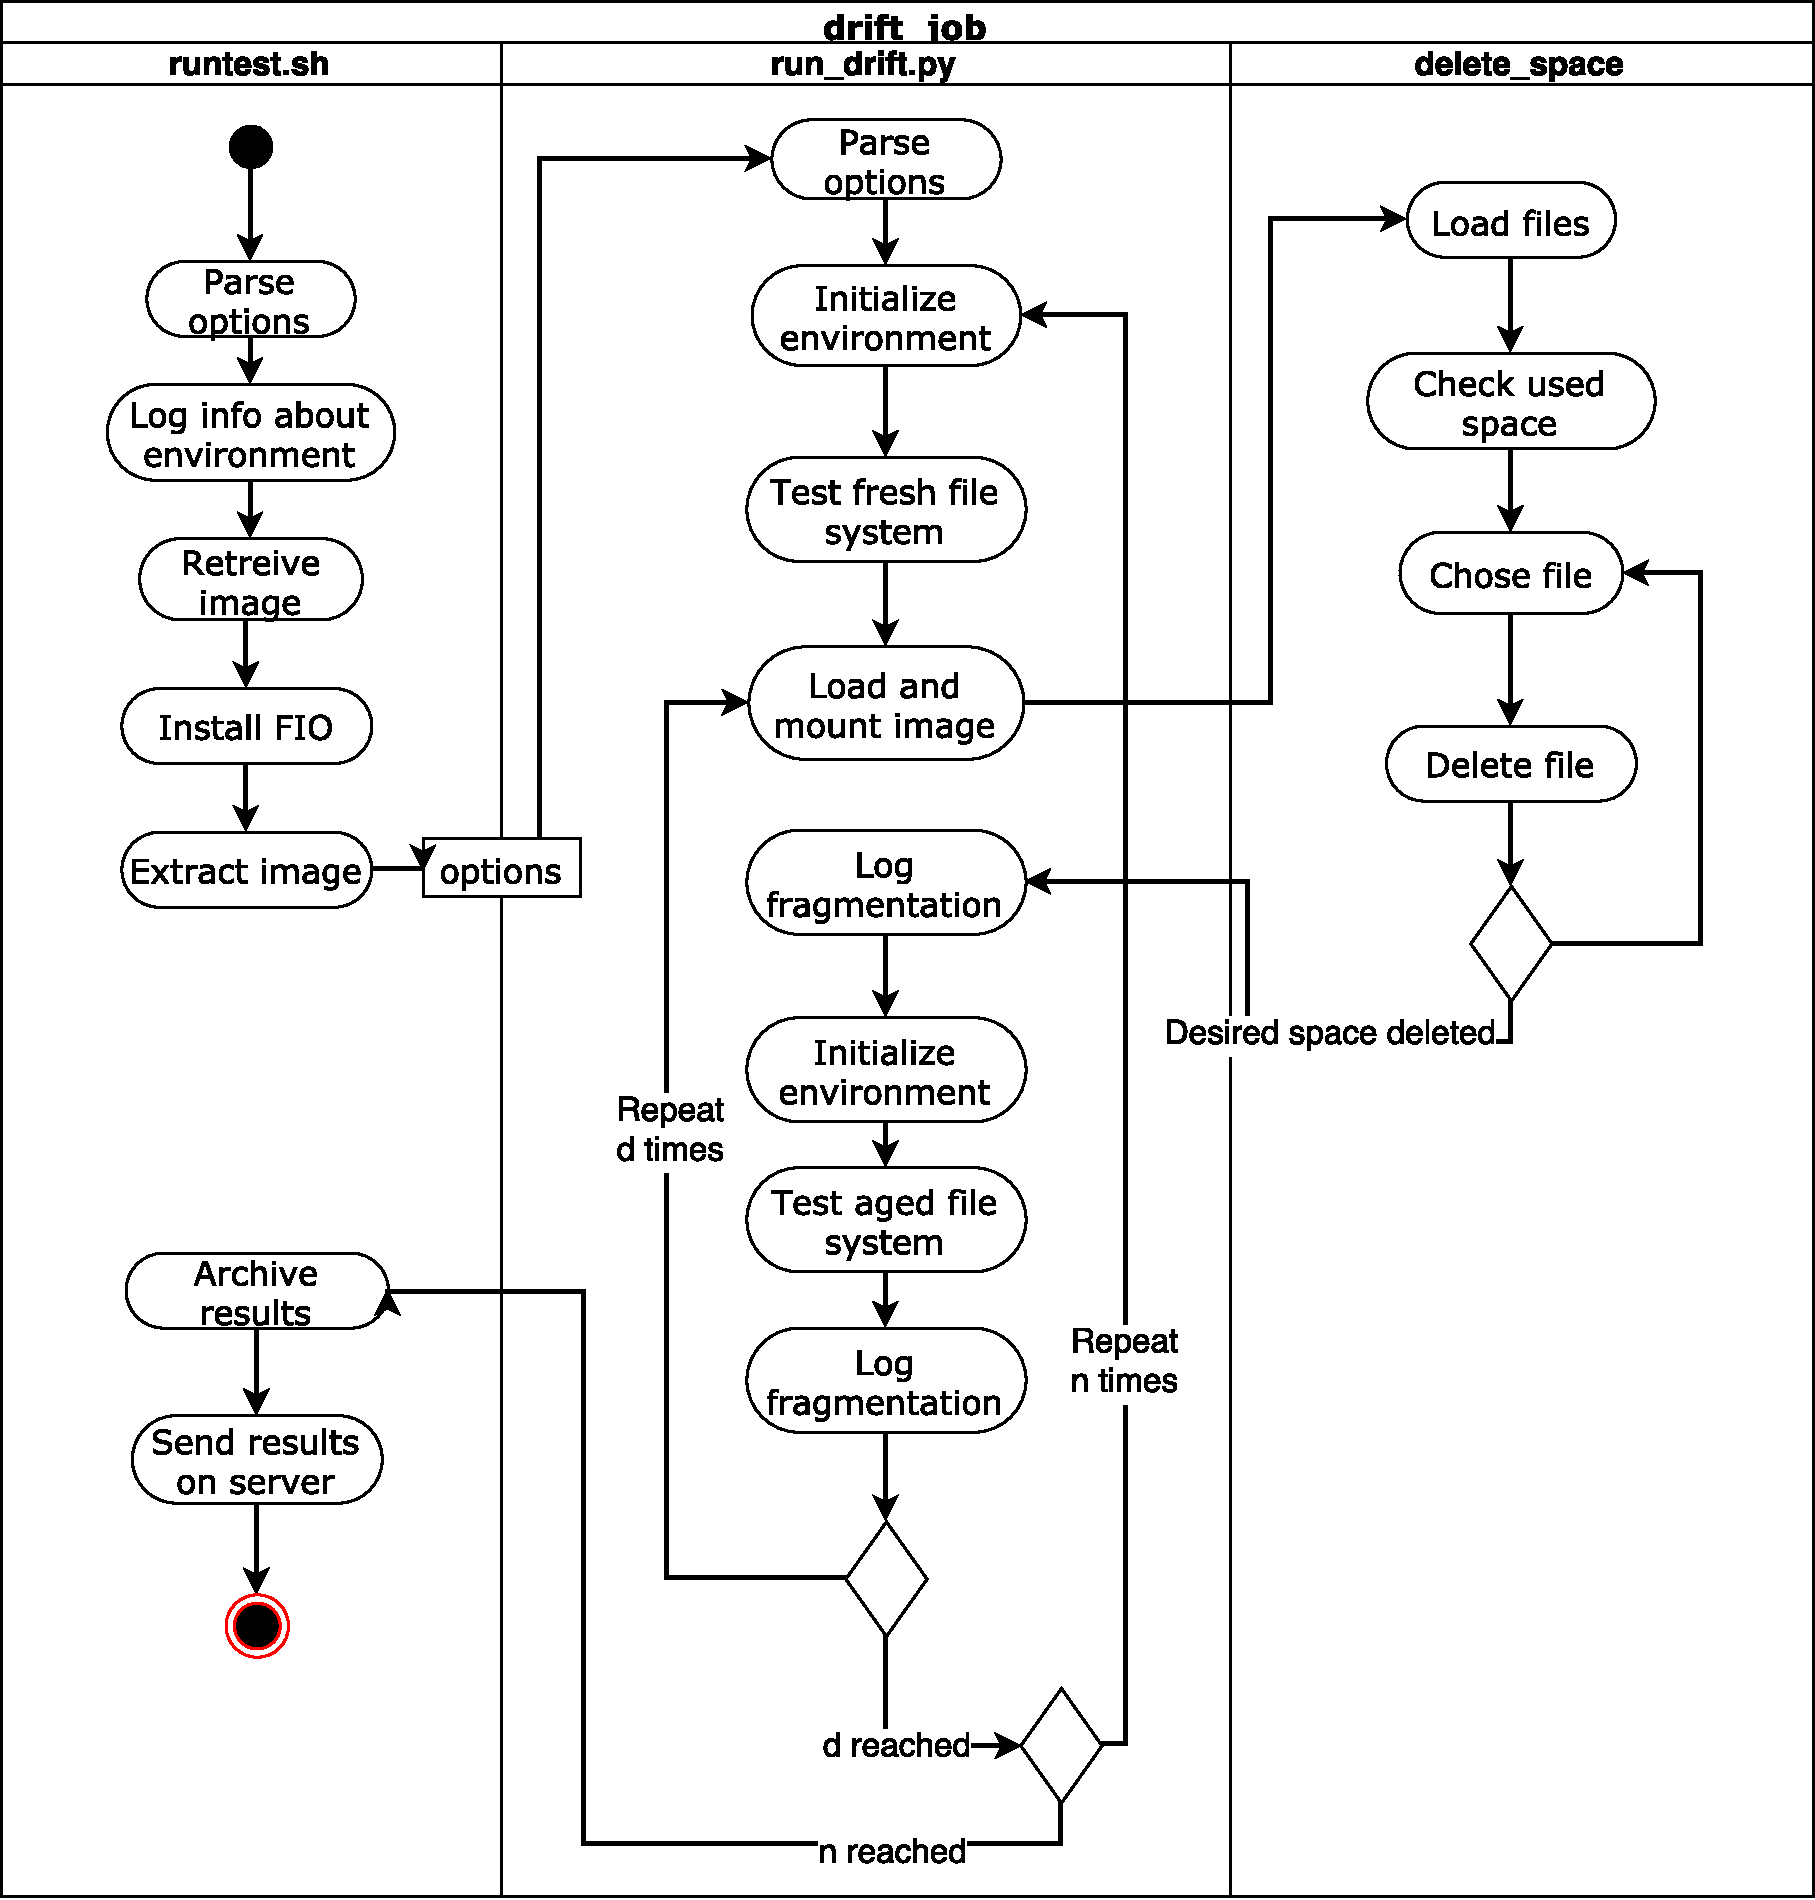
\includegraphics[width=\textwidth,keepaspectratio]{../scripts/recipe_fio_aging_activity}}
    \caption{Activity diagram of testing of aged file system.}
    \label{fig:rec_activity}
\end{figure}







\chapter{Results}
\label{results}
This chapter presents results of implemented tests. In the first section I describe environment used for testing. In the second section, I describe means of data evaluation. In the third section, I show elementary differences between fresh and aged file systems. In the fourth section, I describe differences between two tested file systems (XFS, ext4) in terms of aging. In the fifth section I demonstrate the effect file system aging have on underlying storage.

\section{Testing environment}
\label{env}
The testing machines were available to me from a pool of systems of Red Hat Beaker environment. For every used machine, its model, processor, memory and used storage devices are listed in Table~\ref{machines}.

The OS installed on all Machines were RHEL-7.3 with kernel 3.10.0-514.el7.x86\_64. Tuned profile was set to performance. More information about installed packages can be found in Example~\ref{ex:kickstart}.

\clearpage

\begin{tabular}{|l|l|}
\hline
   \multicolumn{2}{|l|}{Machine\,1} \\ \hline %draven
    Model & Lenovo System x3250\,M6 \\
    \hline
    Processor & Intel Xeon E3-1230\,v5 \\
    \hline
    Clock speed & $\SI{3.40}{\giga\hertz}$ (4 cores) \\
    \hline
    Memory & $\SI{16384}{\mega\byte}$ \\
    \hline
    \multicolumn{2}{|l|}{Storage} \\ \hline
    Device & HP Proliant HardDrive\\ \hline
    Interface & SAS\\ \hline
    Capacity & $\SI{600}{\giga\byte}$\\ \hline
\hline
   \multicolumn{2}{|l|}{Machine\,2} \\ \hline %blade
    Model & Lenovo System x3250\,M6 \\
    \hline
    Processor & Intel Xeon E3-1230\,v5 \\
    \hline
    Clock speed & $\SI{3.40}{\giga\hertz}$ (4 cores) \\
    \hline
    Memory & $\SI{16384}{\mega\byte}$ \\
    \hline
    \multicolumn{2}{|l|}{Storage} \\ \hline
    Device & Intel Solid State Drive \\ \hline
    Interface & SATA\\ \hline
    Capacity & $\SI{120}{\giga\byte}$\\ \hline
\hline
   \multicolumn{2}{|l|}{Machine\,3} \\ \hline %durden
    Model & IBM x3650 System\,M3 \\
    \hline
    Processor & Intel Xeon X5650\,v2 \\
    \hline
    Clock speed & $\SI{2.67}{\giga\hertz}$  (6 cores) \\
    \hline
    Memory &  $\SI{12288}{\mega\byte}$\\
    \hline
    \multicolumn{2}{|l|}{Storage} \\ \hline
    Device & IBM Hard Disk Drive\\ \hline
    Interface &  SAS\\ \hline
    Capacity & $\SI{300}{\giga\byte}$\\ \hline
\end{tabular}
\label{machines}

\section{Data processing}
Accounting for great amount of data generated by the tests, some kind of automatic processing needs to be implemented to make evaluation easier for humans. Therefore, set of scripts which can compare results of two different runs of the test had to be implemented. The output of those scripts is human readable HTML report\footnotemark[1]. The report displays information about testing environment and different charts\footnotemark[2] described bellow. All the charts generated from the tests can be found in the Appendix~\ref{reports}.

\footnotetext[1]{The HTML code is automatically generated using open source library html.py.~\cite{html}}
\footnotetext[2]{Charts were created using JavaScript charting library Highcharts.~\cite{highcharts}}

\subsection{Fragmentation}
During the tests, two types of fragmentation were recorded, namely fragmentation of used space and fragmentation of free space.

To find out the fragmentation of used space, \texttt{xfs\_io fiemap} was used. This tool can display physical mapping of any file, using $\SI{512}{\byte}$ blocks. Therefore, if run on every file in file system, histogram of fragments of used space can be computed. Files created by fs-drift which are smaller then file system block size are nevertheless mapped on one block of file system.

Generally, fragmentation of free space is easier to obtain, since this information is stored in the metadata of file system. However, the way of reading the information differs through implementations of file systems. In ext4, the tool \texttt{e2freefrag} displays histogram of free space of ext file system. When looking for this information in XFS, at~first, user has to find number of allocation groups in the file system instance. Then, for every allocation group, histogram of free space can be obtained using \texttt{xfs\_db}.

As stated in the aging test, fragmentation of free space is logged periodically, allowing for an analysis of how fragmentation evolves in time. For the purpose of visualisation of this evolution, 3D charts are introduced.

\subsection{Evaluation of data generated by fs-drift}
The main researched output of fs-drift is an \emph{evolution} of latency of different operations. This property is displayed as a chart with elapsed time on X axis and measured latency on Y axis. Since the data are quite noisy, interpolation and filtering using Savitzky-Golay filter\footnotemark[1] was used to display smooth curve. Further analysis of obtained data should be done in the future to understand behavior of aged file systems even better. Such deep analysis, however, is beyond scope of this thesis.
\footnotetext[1]{Savitzky-Golay filter is a digital filter used for smoothing noisy data. It is implemented as part of open source scientific tools for Python, SciPy~\cite{scipy}.}

\section{Testing on images of aged file system}
\label{total_hdd}
By testing using second implemented test, no meaningful results were obtained. The observed throughput seemed to be the same across runs on all generated images. The conclusion of this testing is, that it simply does not work as intended. As for testing workflow, images are successfully downloaded, loaded on device and mounted. Afterwards, FIO test is successfully deployed. This can be confirmed from logs generated during the test.

One cause of this problem can be that FIO is simply not suitable for revealing differences between fresh and aged file systems. Another cause of the problem can be in implementation of FIO itself. If there is some bug that causes FIO not to operate as specified by parameters, e.g. FIO will pre-allocate files before performance measuring, the test can output results similar as observed.

Modifying or debugging the benchmark can be a subject of future related work, however such extensive research is beyond scope of this thesis.

%The second implemented test uses images created by the first test to measure state of fragmented, aged file systems. Despite the efforts made while designing benchmark configuration, meaningful results were not obtained from this test. Correct configuration which would prove degraded performance of previously aged file system is yet to be found. Solving such problem requires complex analysis of benchmark and possible debugging. Such efforts can be of subject of future work.


\section{Performance of aged file system}
The file system aging test successfully induced fragmentation in all performed tests. From the data generated by aging test, it is apparent that the aging process negatively affects performance of file systems. Performance degradation varies with used storage, file system implementation and maintenance techniques (e.g. \texttt{fstrim}).

%durden W495 xfs vs draven
On Figure~\ref{fig:free80_xfs}, we can see evolution of fragmentation of free space gathered while testing at medium file system utilisation (80\%). From the Figure~\ref{fig:free99_xfs}, we can see that higher file system utilisation (99\%) induces tremendous fragmentation of free space.

Despite this occurrence, it is remarkable, that fragmentation of used space is very similar across these two test runs. On Figure~\ref{fig:used80_xfs} and~\ref{fig:used99_xfs}, we can see, that both file systems have about 92\% of files optimally allocated. Considering amount of fragments of free space differs in orders of tens of thousands, it is remarkable, that amount of non-contiguous extents of files differs only by 33\%.

On Table~\ref{tab:99_vs_80}, we can see overall raise of latency in regard of highly utilised file system.

Furthermore, operations append and read display signs of progressively larger fluctuations during both tests (Figure~\ref{fig:lats99_xfs} and~\ref{fig:lats80_xfs}). Operations create and truncate show sign of performance degradation only on high utilised file systems (Figure~\ref{fig:lats99_xfs}). Figure~\ref{fig:read_lh} shows comparison of sequential read latencies of medium and highly utilised file system.

\begin{figure}[!htb]
    \centering
   \begin{minipage}{\textwidth}
        \centering
        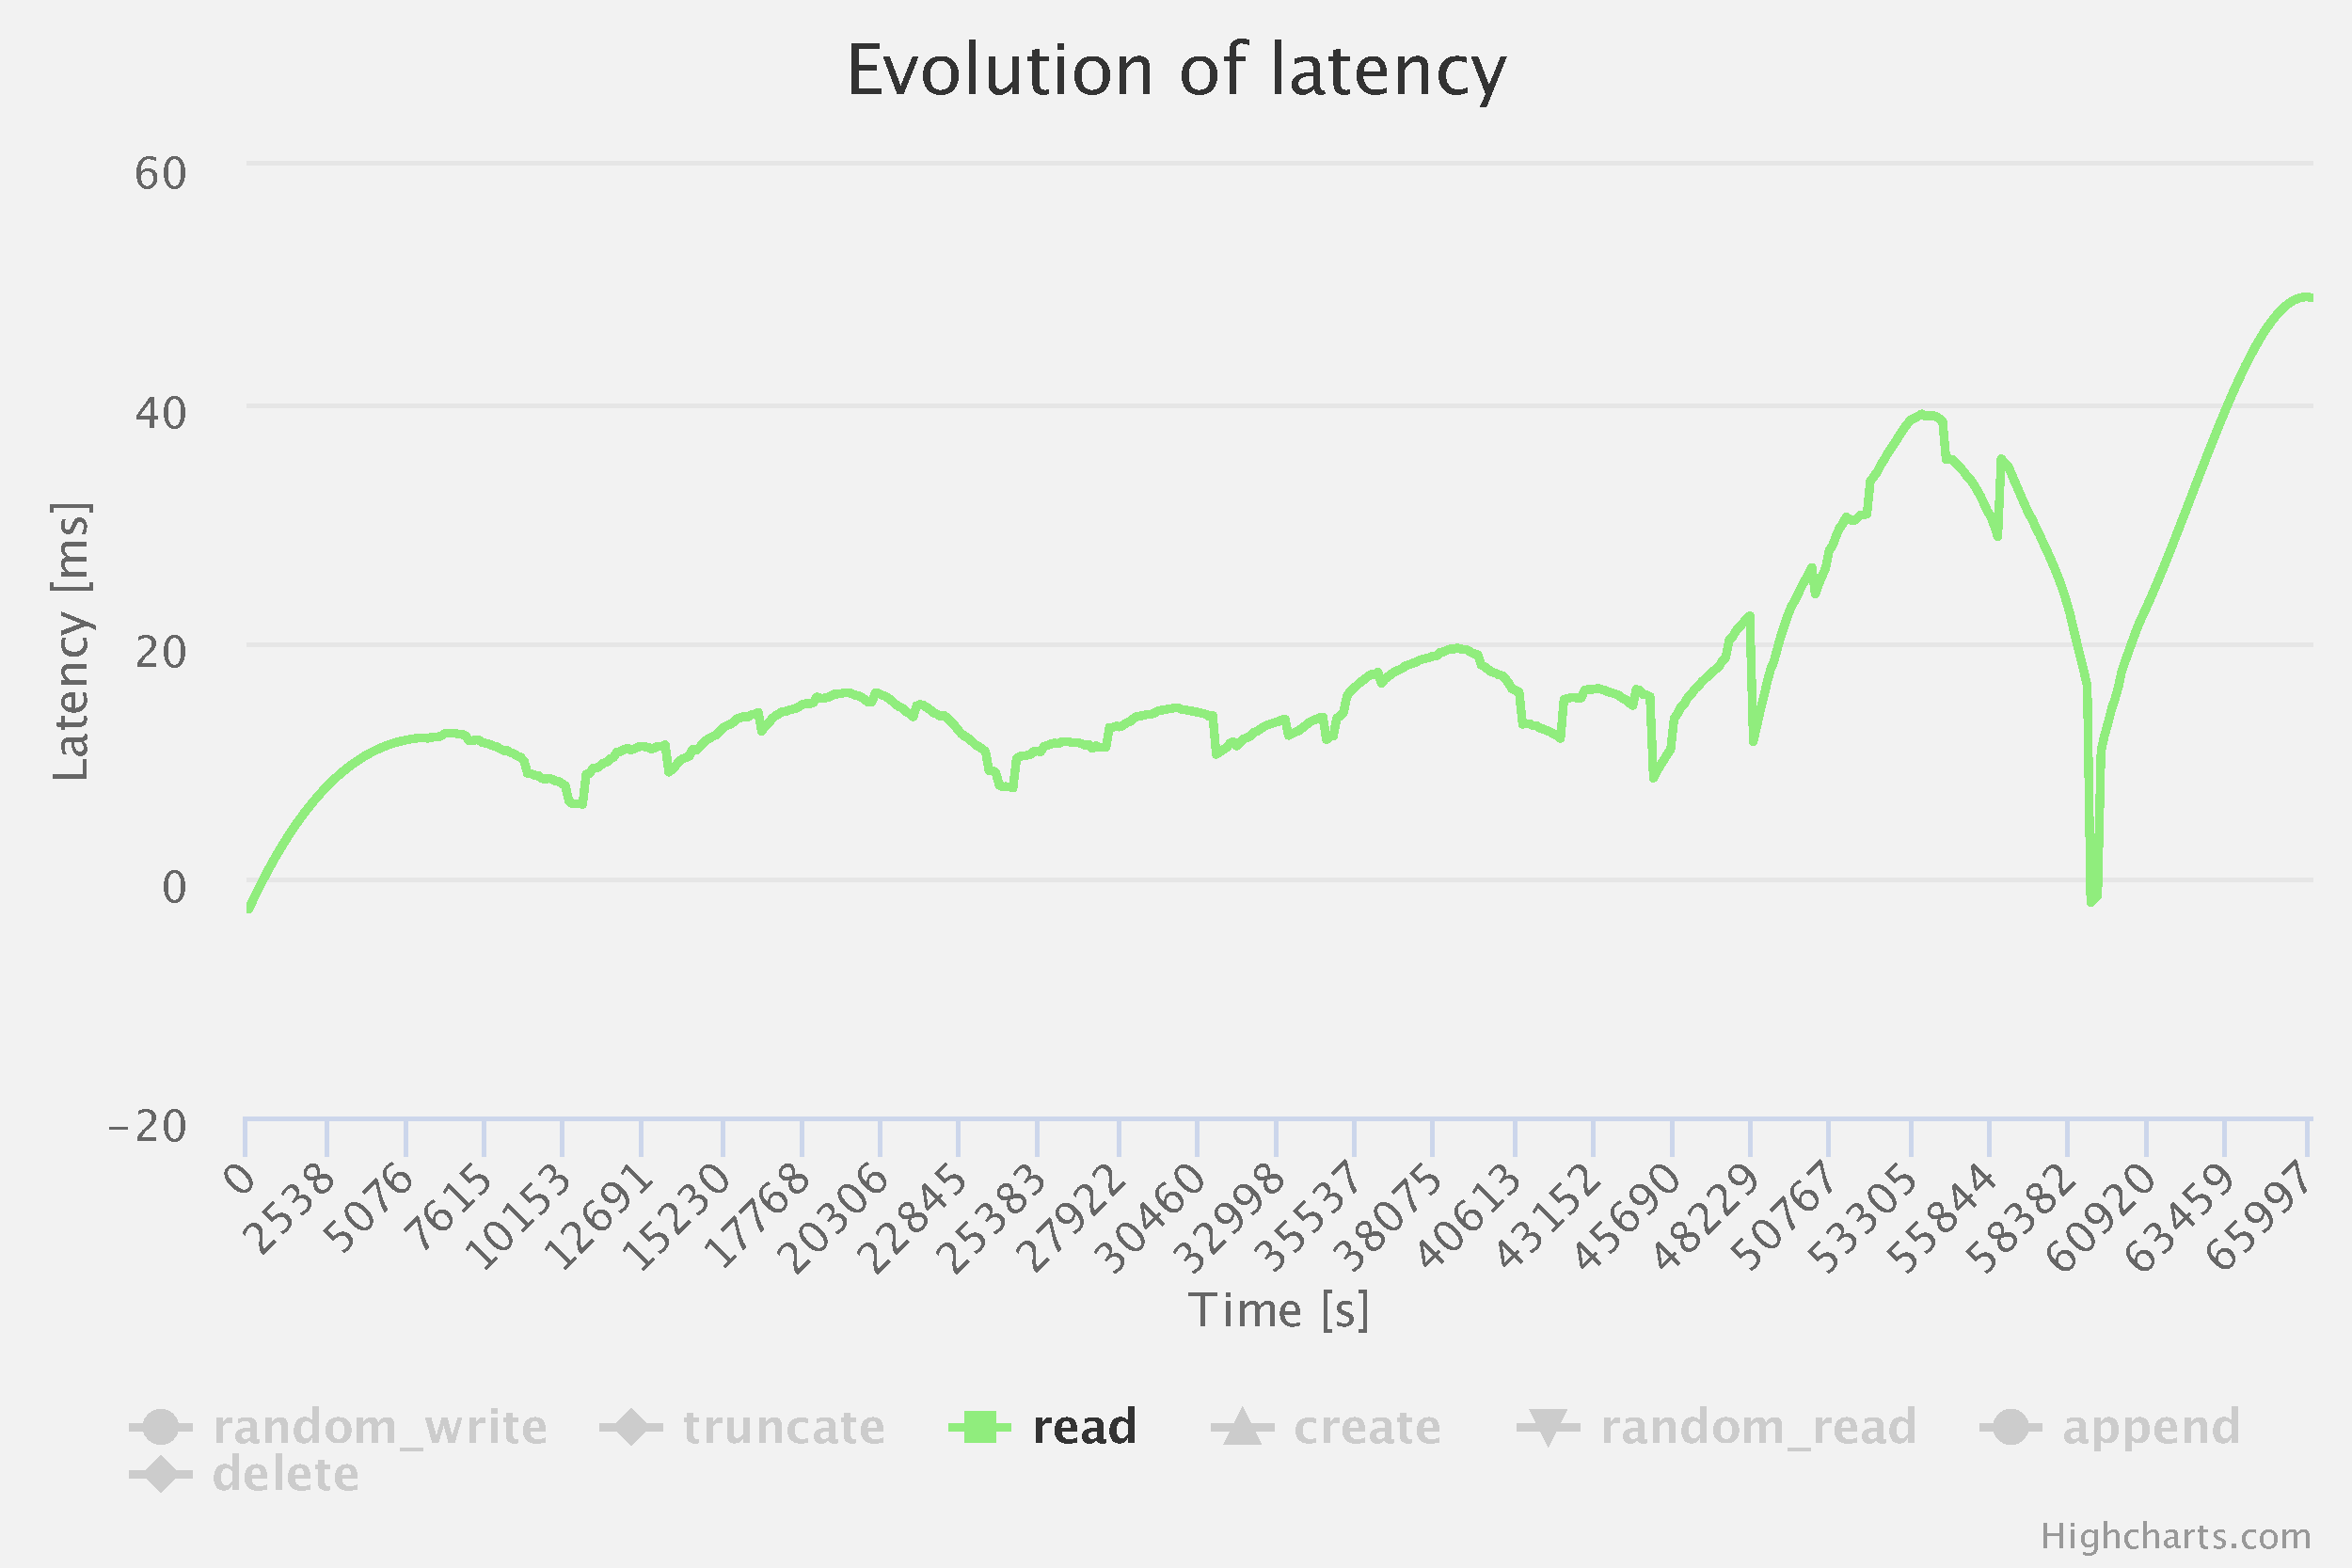
\includegraphics[width=\textwidth]{../charts/HDD_xfs/read_high}
        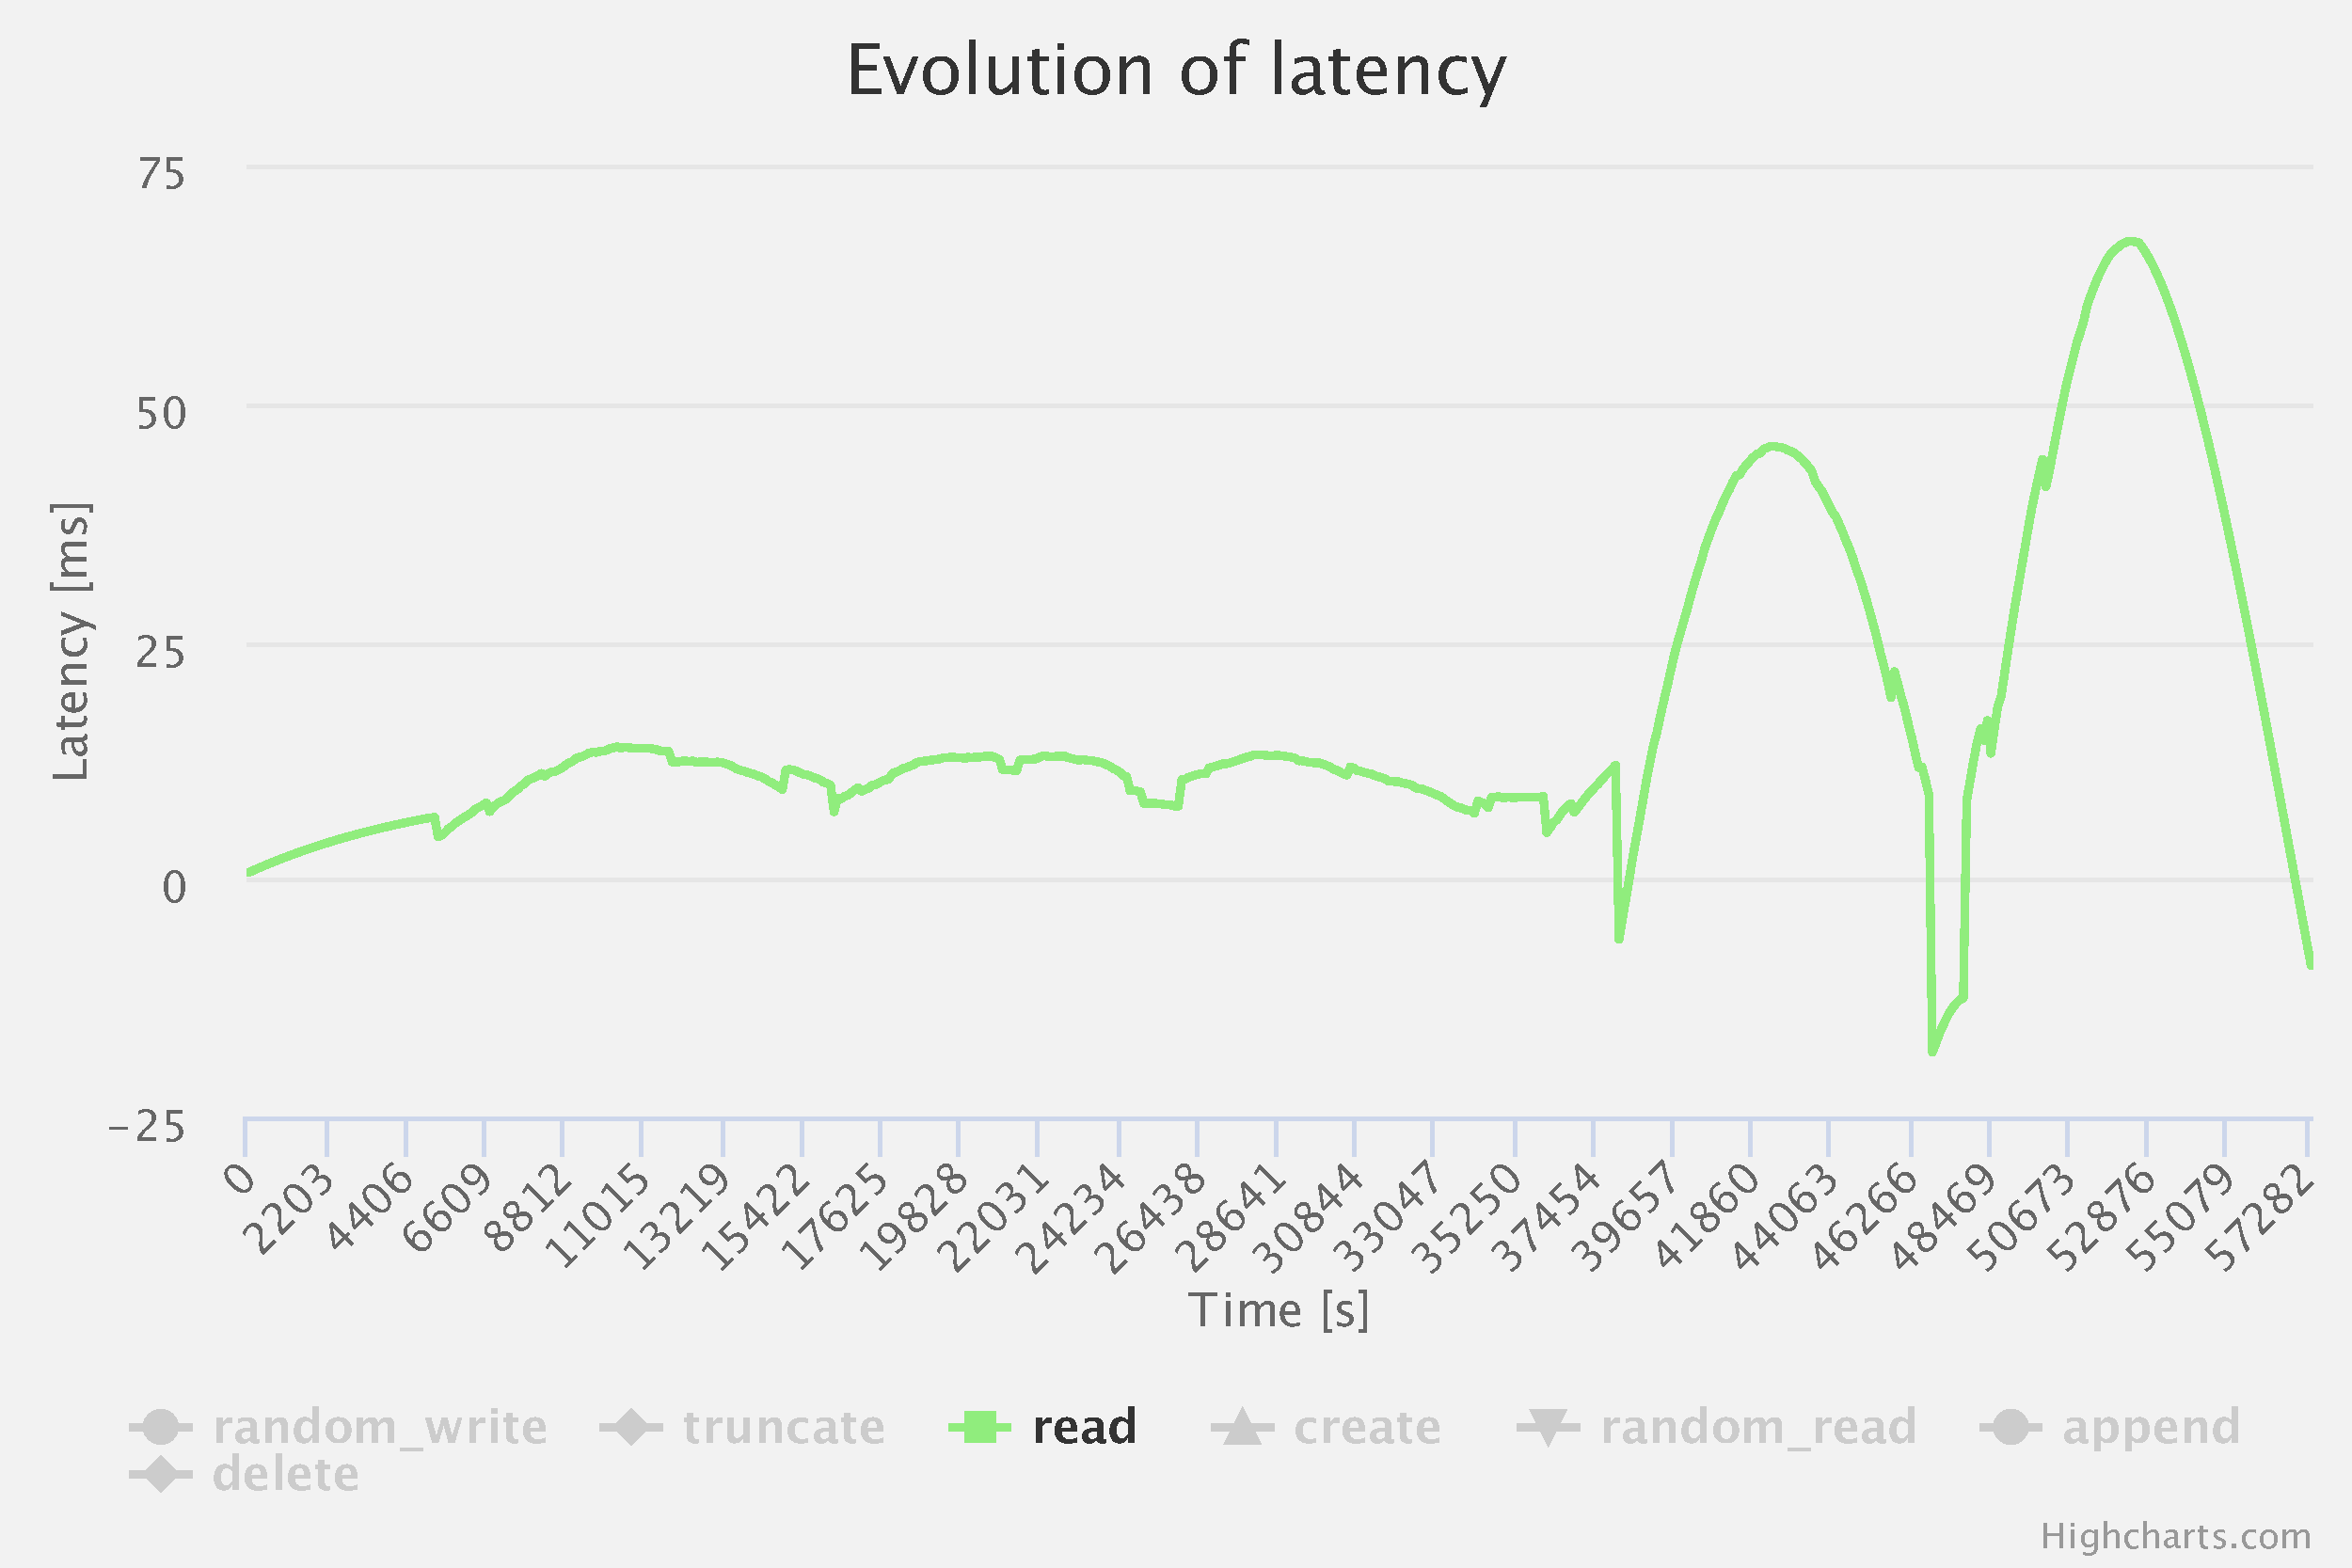
\includegraphics[width=\textwidth]{../charts/HDD_xfs/read_low}
        \caption[Evolution of sequential read of XFS during testing of high and medium utilisation of HDD]{These charts show progressively larger performance fluctuation of sequential read observed on both medium and highly utilised file system.}
\label{fig:read_lh}
    \end{minipage}
\end{figure}

\clearpage

\begin{table}
\centering
\begin{tabular}{|l|l|l|l|}
\hline
 &80\% & 99\% &  \\
\hline
    random write & 11.40\,ms & 11.84\,ms & median \\
 \hline
                 & 16.23\,ms & 17.86\,ms& mean\\
    \hline
        truncate & 8.62\,ms & 8.93\,ms & median\\
    \hline
                 &  10.59\,ms & 11.66\,ms & mean \\
    \hline
           sequential read &  8.03\,ms & 8.54\,ms & median\\
    \hline
                 & 11.20\,ms & 14.30\,ms & mean \\
    \hline
          create & 11.73\,ms & 11.98\,ms & median\\
    \hline
                 & 12.57\,ms & 16.49\,ms & mean \\
    \hline
     random read & 6.42\,ms &6.56\,ms& median\\
    \hline
                 & 7.28\,ms & 8.05\,ms & mean \\
    \hline
          append & 17.66\,ms & 17.93\,ms & median\\
    \hline
                 & 22.00\,ms & 27.30\,ms & mean \\
    \hline
          delete & 0.10\,ms & 0.13\,ms & median\\
    \hline
                & 3.63\,ms & 4.26\,ms & mean \\
    \hline
\end{tabular}
\caption{Comparison of latencies of medium and high utilises file system.}
\label{tab:99_vs_80}
\end{table}


\section{Differences between XFS and ext4}
From the test conducted on highly utilised  HDD, we can conclude that  XFS fights free space fragmentation much better. On a Figure~\ref{fig:free99_xfs}, which shows last 6 hours of testing high utilisation of XFS on HDD, we can see relatively low amount of free space extents. The peaks in number of extents are caused by random space releasing conducted by aging test, which can be confirmed by examining corresponding usage evolution chart (Figure~\ref{fig:used99_xfs}). After every peak occurrence, it is clear that number of small extents is progressively lowered until the next peak. It is clear that XFS successfully defragments free space between the volume releasing iterations. On the other hand, while examining evolution of free space fragmentation of ext4 (Figure~\ref{fig:free99_ext4}, last 6 hours of the test), we can see that after volume releasing, the amount of small extents of free space remain more or less the same. Furthermore, through most of the testing time, ext4 contained about 20 thousands of extents of free space, which is significantly more than XFS.

Such free space fragmentation can have significant impact on overall file system performance. This can be observed in spite of block allocation operations such as create and append, as we can see in Table~\ref{tab:hdd_ssd_xfs_ext4}.
%From the graph of evolution of free space fragmentation, it is apparent, that XFS fights free space fragmentation significantly better than Ext4. On the Figure~\ref{fig:hdd_xfs_free_frag} we can see, that XFS tries to maximise size of free space blocks. Even at the end of testing stage, XFS still operates with large blocks of free space (up to $\SI{63}{\giga\byte}$).

%By default, Ext4 operates with size of free blocks no larger than $\SI{2}{\giga\byte}$. With greater utilisation of file system, induced fragmentation of free space is visible. At the end of the test, Ext4 operates with up to nine thousands of fragments of free space, as can be seen on Figure~\ref{fig:hdd_ext4_free_frag}.

%\subsection{XFS and EXT4 on SSD}
%SSD xfs vs SSD ext4
%Fragmentacia volneho aj pouziteho miesta priblizne rovnaka. Optimalnych filov u oboch 98\%. Rozlozenie fragmentov, v ext4 je malo stredne velkych fragmentov. Randwrite neaguje, obcas vyskoci, hodnoty podobne. Truncate slaby aging, hodnoty podobne. Read, XFS rychlejsie, resp nema take peaky ako ext4, ale zda sa, ze je tam nejake stupanie na rozdiel od ext4. Create bez agingu, ale xfs sa zda pomalsie (treba skontrolovat hodnoty). Rand read, bez agingu, xfs sa zda pomalsie, ale mozno len koli jednomu peaku. Append bez agingu. Ext4 vacsi peak, ale mozno nizsie hodnoty. Delete, xfs rychlejsie, ext4 velke peaky, chekni hondoty.
When testing with SSD, XFS and ext4 have very similar disk layouts in spite of free and used space fragmentation. After maximal disk utilisation is reached, both file systems have up to 50\,000 fragments of free space (Figure~\ref{fig:free_xfs_ssd_trim} and Figure~\ref{fig:free_ext4_ssd}). At the end of the test, both file systems had 98\% of files optimally allocated. The only difference when considering block layout seems to be in size distribution of extents. As can be seen on Figure~\ref{fig:used_xfs_ssd_trim} and Figure~\ref{fig:used_ext4_ssd}, ext4 has more smaller fragments than XFS. Since continuity of relevant blocks may play role even while using SSD, this could mean potential performance penalty.

In Table~\ref{tab:hdd_ssd_xfs_ext4}, we can see median and mean of all operations through the whole test. It is clear that all the operations except delete and truncate are slightly faster if performed by XFS. This small difference can be result of lesser used space fragmentation in XFS.

\begin{table}
\centering

\begin{tabular}{|l|l|l|l|l|l|}
\hline
   & \multicolumn{2}{|c|}{SSD} & \multicolumn{2}{|c|}{HDD} & \\ \hline

 & \multicolumn{1}{|c|}{XFS} & \multicolumn{1}{|c|}{ext4} & \multicolumn{1}{|c|}{XFS} & \multicolumn{1}{|c|}{ext4} &  \\
\hline
    random write & 0.434\,ms & 0.594\,ms & 11.84\,ms & 11.20\,ms & median\\
 \hline
                 & 1.40\,ms & 3.05\,ms & 17.86\,ms & 18.95\,ms & mean\\
    \hline
        truncate & 0.70ms & 0.32\,ms & 8.93\,ms & 5.22\,ms & median\\
    \hline
                 & 1.48\,ms & 1.35\,ms& 11.66\,ms & 5.84\,ms & mean\\
    \hline
           sequential read & 1.37\,ms & 1.56\,ms & 8.54\,ms & 7.64\,ms & median\\
    \hline
                 & 3.24\,ms & 3.47\,ms & 14.30\,ms & 10.96\,ms & mean\\
    \hline
          create & 0.38\,ms & 0.40\,ms & 11.98\,ms & 18.19\,ms & median\\
    \hline
                 & 4.02\,ms & 3.84\,ms & 16.49\,ms & 19.36\,ms & mean\\
    \hline
     random read & 0.3\,ms & 0.46\,ms & 6.56\,ms & 5.50\,ms & median\\
    \hline
                 & 1.32\,ms & 1.37\,ms & 8.048\,ms  & 6.11\,ms &mean\\
    \hline
          append & 1.49\,ms & 1.76\,ms & 17.93\,ms & 23.81\,ms & median \\
    \hline
                 & 6.46\,ms & 6.65\,ms & 27.29\,ms & 28.36\,ms &mean\\
    \hline
          delete & 0.097\,ms & 0.049\,ms & 0.128\,ms & 0.091\,ms & median\\
    \hline
                & 0.701\,ms & 0.346\,ms & 4.26\,ms & 1.32\,ms & mean\\
    \hline
\end{tabular}
\caption{Comparison of latencies gathered during testing with XFS and ext4 on SSD and HDD.}
\label{tab:hdd_ssd_xfs_ext4}
\end{table}



%\subsection{XFS and EXT4 on 600\,GB HDD}
%600 HDD xfs vs 600 HDD ext4
%Lebo mali file systemy vela miesta, tak velmi nefragmentovali, optimalnych filov je 99\%, ale u xfs to vyzera, ze fragmentovalo viacej, POZOR FIEMAP MALO ZALOGOVAL. Kazdopadne ma menej fragmentov volneho miesta, %radovo desiatky, ext4 ma tisicky.
%Vyzera to, ze xfs ma pomalsi randwrite, aj ked treba ceknut hodnoty, inak aging sa neprejavuje. Truncate, aging sa prejavuje, xfs pomalsie. Read, xfs o cosi pomalsie, aging sa prejavuje. Create, aging sa asi neprejavuje, chce to lepsi graf, inak xfs vyzera horsie. Random read, xfs horsie, aging sa prejavuje. Append, aging sa neprejavuje, len vyskocil, mozno ext4 trochu horsie. Delete xfs horsi, agung sa asi neprejavuje.

%While testing on large HDDs, aging tests were unable to fill devices in reasonable time. Despite the fact the devices were utilised to 80-85\%, file system performance degradation could have been observed

\section{Performance accross different storage devices}
Underlying storage has significant impact on file system performance. As mentioned, SSDs lack of moving parts allows the file system to perform IO faster. Even when connected through a slower (SATA) interface than HDD (SAS), SSD issues operations much faster, as we can see in Table~\ref{tab:ssd_hdd_xfs}. Despite the difference in overall speed of the devices, underlying storage technology have apparently no effect on fragmentation, because file systems deploy the same defragment strategies in both cases. However, latency grow observed on HDD, as mentioned in Section~\ref{total_hdd} was not observed when testing on SSD.

\begin{table}
\centering
\begin{tabular}{|l|l|l|l|}
\hline
 &HDD & SSD &  \\
\hline
    random write & 11.84\,ms & 0.43\,ms & median \\
 \hline
                 & 17.86\,ms & 1.41\,ms & mean\\
    \hline
        truncate & 8.93\,ms & 0.70\,ms & median\\
    \hline
                 & 11.67\,ms & 1.47\,ms & mean \\
    \hline
           sequential read & 8.54\,ms & 1.37\,ms & median\\
    \hline
                 & 14.30\,ms & 3.24\,ms & mean \\
    \hline
          create & 11.98\,ms & 0.33\,ms & median\\
    \hline
                 & 16.49\,ms & 4.02\,ms & mean \\
    \hline
     random read & 6.56\,ms & 0.29\,ms & median\\
    \hline
                 & 8.04\,ms & 1.32\,ms & mean \\
    \hline
          append & 17.93\,ms & 1.49\,ms & median\\
    \hline
                 & 27.29\,ms & 6.47\,ms & mean \\
    \hline
          delete & 0.128\,ms & 0.097\,ms & median\\
    \hline
                & 4.26\,ms & 0.70\,ms & mean \\
    \hline
\end{tabular}
\caption{Comparison of latencies of gathered during aging test on HDD and SSD.}
\label{tab:ssd_hdd_xfs}
\end{table}

\section{Testing with \texttt{fstrim}}
All the mentioned results generated by tests conducted on SSD devices had regular trimming scheduled as a part of the test. However, experimental test runs without trimming were also conducted. 

From the tests, it is apparent, that regular running of \texttt{fstrim} have indeed beneficial effects on file system performance. The most affected operation was create while testing the XFS. Apparent latency growth of create can be seen in Figure~\ref{fig:notrim_create}. Overall difference in latencies can be found in Table~\ref{tab:trim}.

Trimming should not have any effects on fragmentation of file systems, but a difference can be seen in the overall used space fragmentation. While both file systems (trimmed and not trimmed) have similar percentage of optimally allocated files, file system that was not trimmed contains significantly smaller amount of fragments and larger average fragment than trimmed file system (Figure~\ref{fig:used_xfs_ssd_trim} and~\ref{fig:used_xfs_ssd_notrim}). This could be explained by a great latency of untrimmed device, which may have resulted for file system to have more time to schedule written blocks better.

This result is great example of testing long-term performance affecting features by using aging test, as well as importance of regular trimming of SSD devices.


\begin{figure}
    \centering
    \fbox{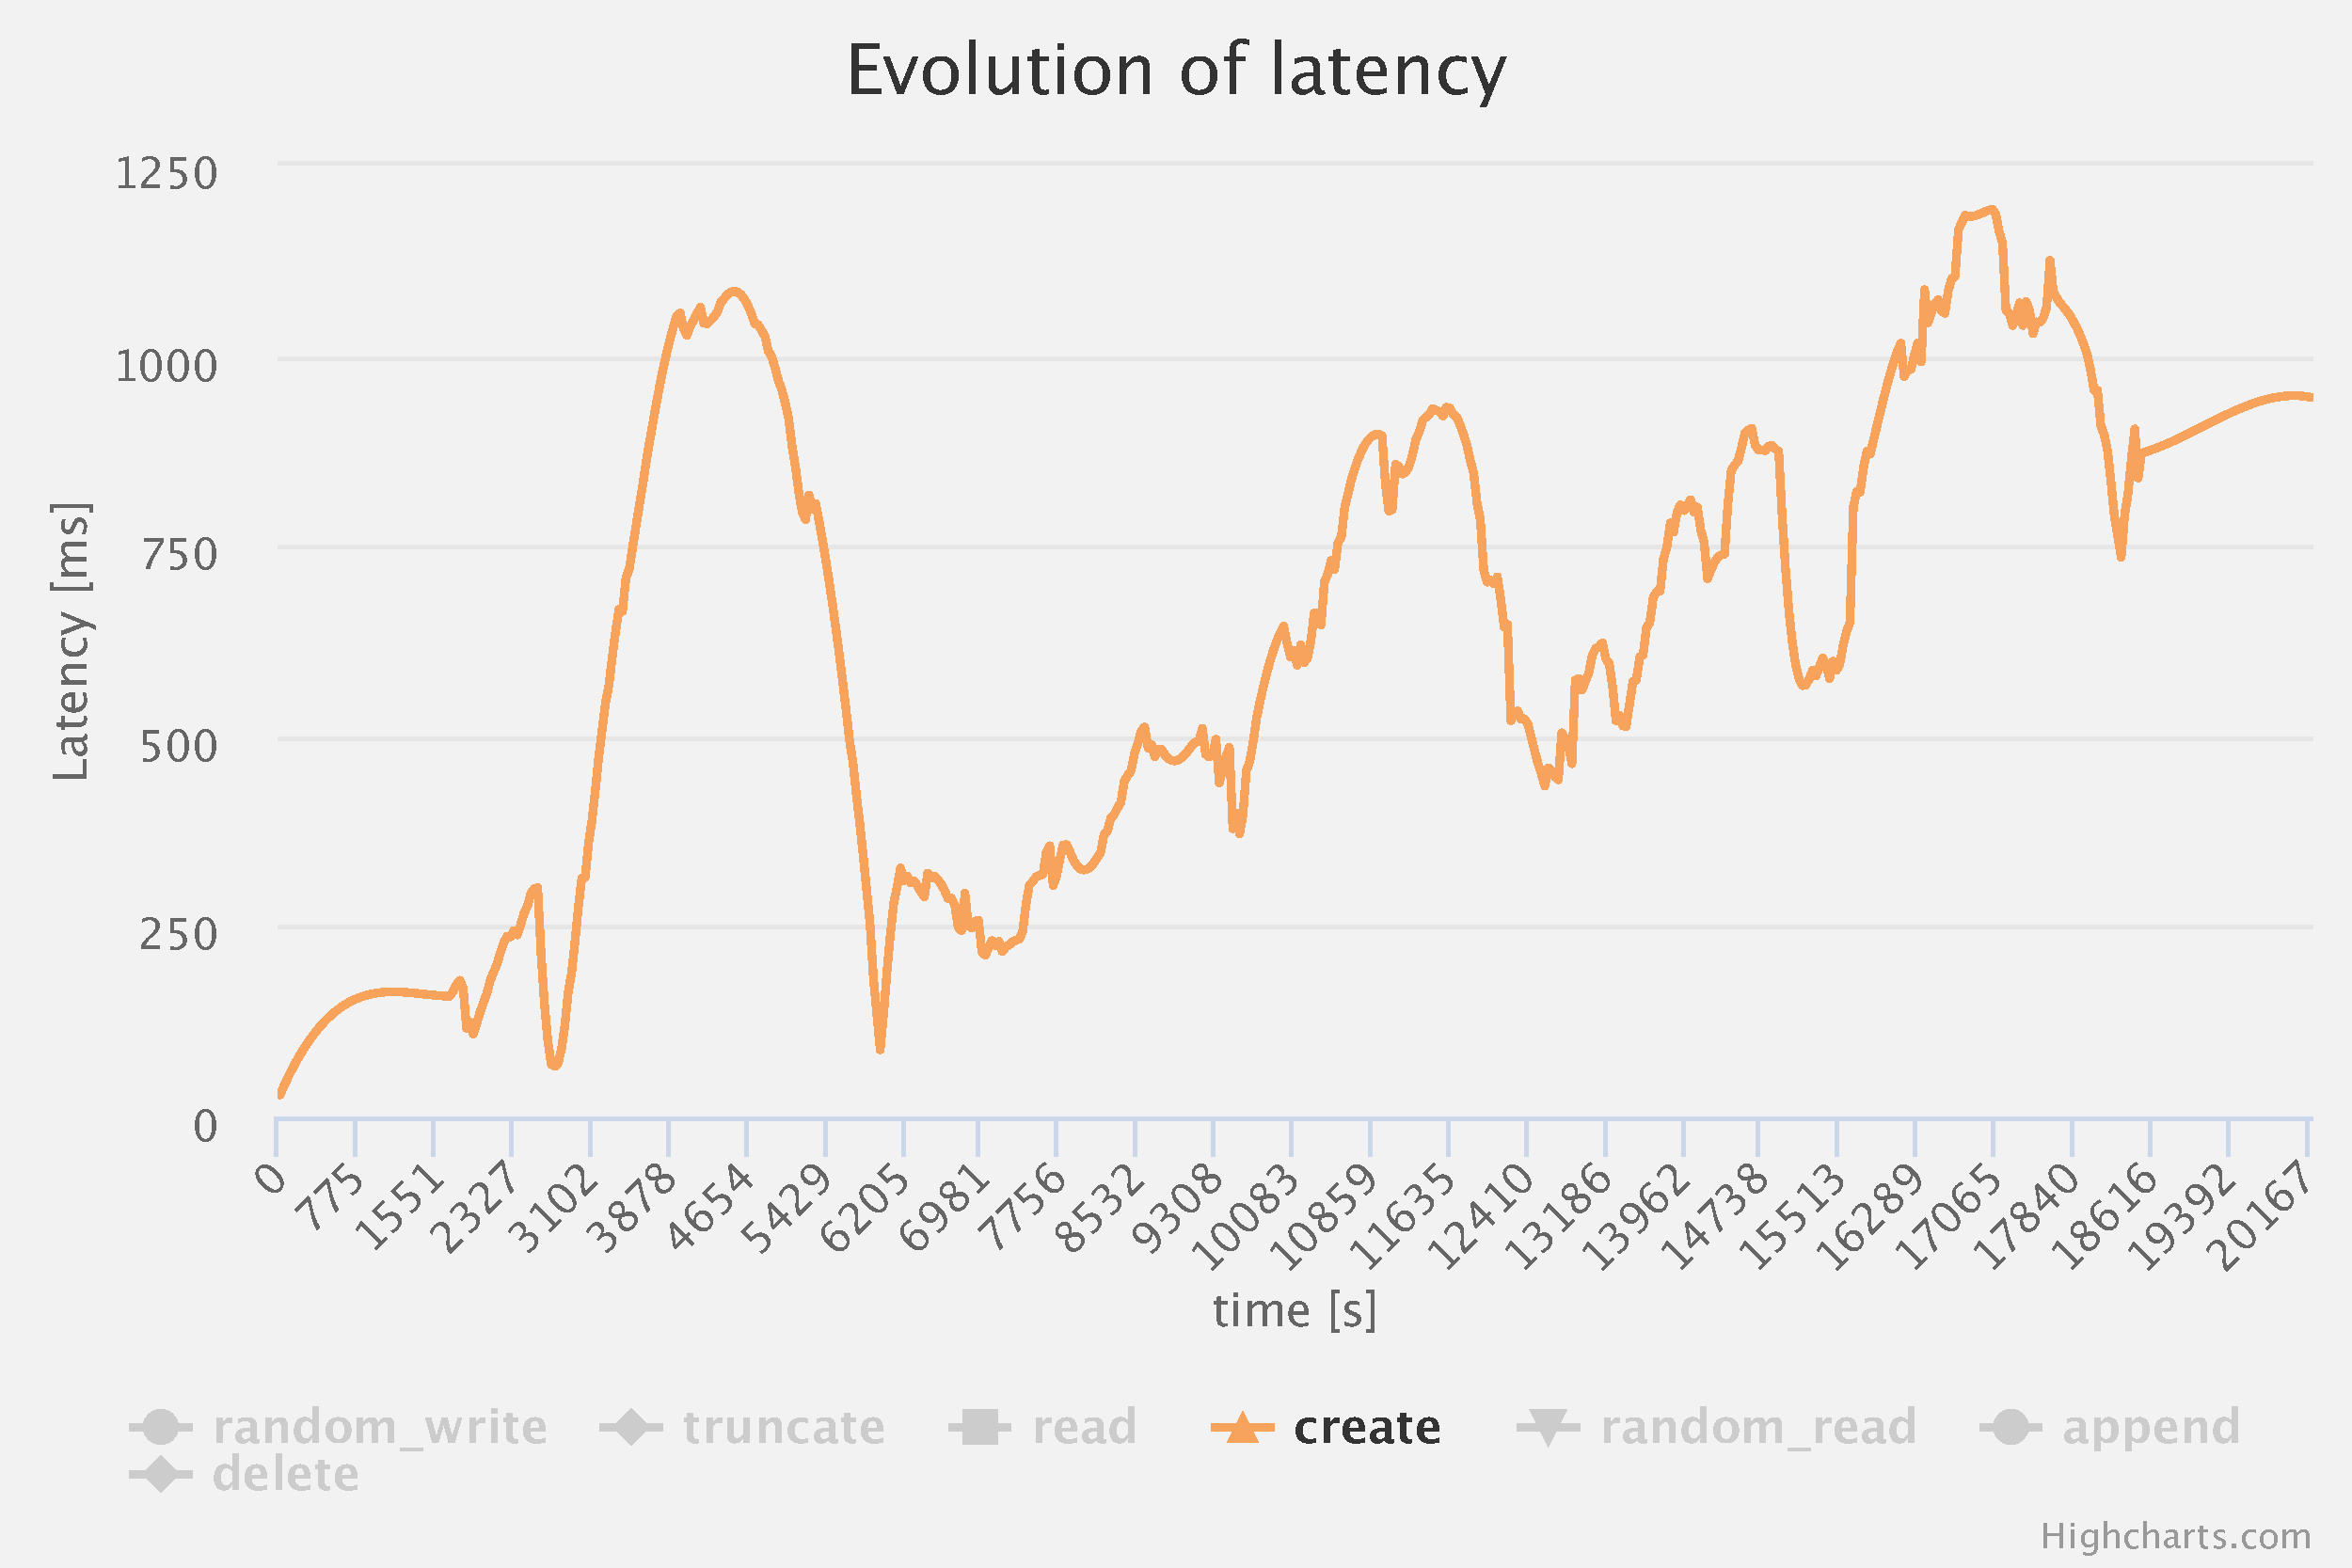
\includegraphics[width=\textwidth,keepaspectratio]{../charts/SSD_xfs_notrim/create}}
    \caption[Evolution of latency of create operation, in untrimmed file system (XFS)]{Latency evolution of create operation, in untrimmed XFS.}
    \label{fig:notrim_create}
\end{figure}

\begin{table}
\centering
\begin{tabular}{|l|l|l|l|}
\hline
 &Trimmed & Not trimmed &  \\
\hline
    random write & 0.43\,ms & 0.52\,ms & median \\
 \hline
                 & 1.40\,ms & 4.99\,ms & mean\\
    \hline
        truncate & 0.70\,ms & 1.05\,ms & median\\
    \hline
                 & 1.48\,ms & 3.17\,ms & mean \\
    \hline
           sequential read & 1.37\,ms & 1.85\,ms & median\\
    \hline
                 & 3.24\,ms & 4.74\,ms & mean \\
    \hline
          create & 0.33\,ms & 0.34\,ms & median\\
    \hline
                 & 4.02\,ms & 6.02\,ms & mean \\
    \hline
     random read & 0.30\,ms & 0.38\,ms & median\\
    \hline
                 & 1.32\,ms & 1.99\,ms & mean \\
    \hline
          append & 1.49\,ms & 1.99\,ms & median\\
    \hline
                 & 6.47\,ms & 8.33\,ms & mean \\
    \hline
          delete & 0.097\,ms & 0.102\,ms & median\\
    \hline
                & 0.70\,ms & 0.97\,ms & mean \\
    \hline
\end{tabular}
\caption{Differences in latencies of trimmed and not trimmed file system (XFS).}
\label{tab:trim}
\end{table}

%Running \texttt{fstrim} regularly through the test has significant impact on performance on operations create and append. Those operations create IO requests sequentially, so it is expected


%POZNAMKY, CO VIDIM Z POROVNANI
%Vsetky pouzite SSD vysledky su TRIM

%Filesystemy
%NVME xfs vs NVME ext4
%***cakame na NVME ext4***

%SSD xfs vs SSD ext4
%Fragmentacia volneho aj pouziteho miesta priblizne rovnaka. Optimalnych filov u oboch 98\%. Rozlozenie fragmentov, v ext4 je malo stredne velkych fragmentov. 
%Randwrite neaguje, obcas vyskoci, hodnoty podobne. Truncate slaby aging, hodnoty podobne. Read, XFS rychlejsie, resp nema take peaky ako ext4, ale zda sa, ze je tam nejake stupanie na rozdiel od ext4. Create bez agingu, ale xfs sa zda pomalsie (treba skontrolovat hodnoty). Rand read, bez agingu, xfs sa zda pomalsie, ale mozno len koli jednomu peaku. Append bez agingu. Ext4 vacsi peak, ale mozno nizsie hodnoty. Delete, xfs rychlejsie, ext4 velke peaky, chekni hondoty.


%600 HDD xfs vs 600 HDD ext4
%Lebo mali file systemy vela miesta, tak velmi nefragmentovali, optimalnych filov je 99\%, ale u xfs to vyzera, ze fragmentovalo viacej, ale moze to byt tym, ze stihlo viac zaplnit disk (85\% oproti 79\%). Kazdopadne ma menej fragmentov volneho miesta, radovo desiatky, ext4 ma tisicky.
%Vyzera to, ze xfs ma pomalsi randwrite, aj ked treba ceknut hodnoty, inak aging sa neprejavuje. Truncate, aging sa prejavuje, xfs pomalsie. Read, xfs o cosi pomalsie, aging sa prejavuje. Create, aging sa asi neprejavuje, chce to lepsi graf, inak xfs vyzera horsie. Random read, xfs horsie, aging sa prejavuje. Append, aging sa neprejavuje, len vyskocil, mozno ext4 trochu horsie. Delete xfs horsi, agung sa asi neprejavuje.



%STORAGE:
%NVME xfs vs SSD xfs
%Nvme, lebo je 400GB muselo vytvorit viac filov, preto ma aj vacsi pocet fragmentov, optimalnych filov je 88\% oproti 98 pri SSD.
%sdcko vykonalo 6 milionov operacii za 9000 sekund, nvme vykonalo 10 milionov operacii za 12000 sekund, to znamena, ze vykonalo za 9000 sekund 8.5 miliona operacii.
%Vidime, ze ked doslo volne miesto, velmi sa nafragmentoval
%Randwrite omnoho rychlejsi, ale aging sa neprejavuje ani u jednoho. Truncate stabilny.
%Aging readu sa prejavuje u obidvoch, vysledky z nvme su nestabilne, velke skoky. Create rychlejsi, s tym, ze aging sa neprejavuje. Random read stabilne rychlejsi. Append sa javi rychlejsi v SSD. Delete neaguje, nvme je rychlejsie.

%NVME ext4 vs SSD ext4
%***cakame na NVME ext4 ***


%SSD_xfs vs 300 HDD xfs
%***cakame 300 HDD xfs***

%SSD ext4 vs 300 HDD ext4




\chapter{Conclusion}
\label{conclusion}
%Tesing of file system aging is complex and challenging problem.

The aim of this thesis was to introduce means of testing of file system aging performance. This goal was reached by creating two automated tests, which use existing benchmarks for testing.

The file system aging test use workload generator to simulate aging. Because test is automated, environment configuration has to be done as well as tool preparation. While aging, the test gathers lots of data and statistics about file system usage, fragmentation levels and performance of conducted IO operations. After the test, metadata images of file systems are successfully automatically created and compressed. 

This file system aging test successfully induce fragmentation and aging of used file systems. From the generated data, it can be observed, that aging indeed causes performance penalty on file systems. These effects were observed in both tested file systems.



%However, deeper data analysis would have to be performed to fully understand the evolution of performance through aging, yet such analysis is beyond scope of this thesis.

%The second implemented test uses images created by the first test to measure state of fragmented, aged file systems. Despite the efforts made while designing benchmark configuration, meaningful results were not obtained from this test. Correct configuration which would prove degraded performance of previously aged file system is yet to be found. Solving such problem requires complex analysis of benchmark and possible debugging. Such efforts can be of subject of future work.

Further aim of this thesis was to compare performance of different aged file systems and effect of used storage technologies on performance.

From the obtained data, it is apparent that with higher utilisation of file systems, performance degrading effects becomes observable. Even while using flash based devices (i.e. SSD), the aging can have degrading effect on performance of some IO operations.

%By testing and comparing XFS and EXT4 file systems, several differences can be found,

Furthermore, this test was used to demonstrate effects of long term performance affecting tool \texttt{fstrim}, displaying another use case of this test besides evaluation of file system implementation itself.

% both file systems can be considered evenly performing and suitable for long term deployment.  

This thesis was aimed on testing so called local file systems with simple configuration, which means the whole drive is presented to file system as a single block device. However, storage usage is evolving into new approaches. Cloud solutions are becoming more and more popular, therefore file systems, which operate over storage clusters are already in production (e.g. CephFS\footnotemark[1]). Such file systems have to deal with many new problems like working with metadata, which are stored on remote server, or distribute data evenly accross the cluster.

\footnotetext[1]{Ceph storage cluster file system.\cite{weil2006ceph}}

Virtualisation also requires new solutions and additional performance control. With development of tools like LVM, it is possible to merge multiple devices into huge, flexible arrays. Approaches like thin-provisioning then offer further possibilities of providing storage space to users. 

With such growing complexity, file system aging (and software aging generally) can have significant impact on performance of these systems. It is, therefore, very important to research and understand complex behavior of file system aging.

The automated file system aging test and means of evaluation of generated data are the main results of this thesis. Since the aging test was implemented as a Beaker task, it is compatible with Red Hat Kernel Performance team workflow and was therefore included in testing matrix of Red Hat Enterprise Linux 7.4 and Pegas and upstream kernels. Including this test in regular testing matrix is an important step in expanding ways of examining file systems in new kernel versions. Testing file system aging may reveal and help repair complex problems which can emerge during file systems development.

The results of this thesis were presented to developers of file systems and open source community as well. Future plans for file system aging are discussed with developers of file systems.




\printbibliography[heading=bibintoc]















\appendix %% Start the appendices.
\chapter{Reports}\label{reports}



\section{Test of medium utilisation using XFS on HDD}

\begin{itemize}
\itemsep0em 
   \item System: Machine\,1
   \item OS: RHEL-7.3
   \item Kernel: 3.10.0-514.el7.x86\_64
\end{itemize}


\begin{figure}[!htb]
        \centering
        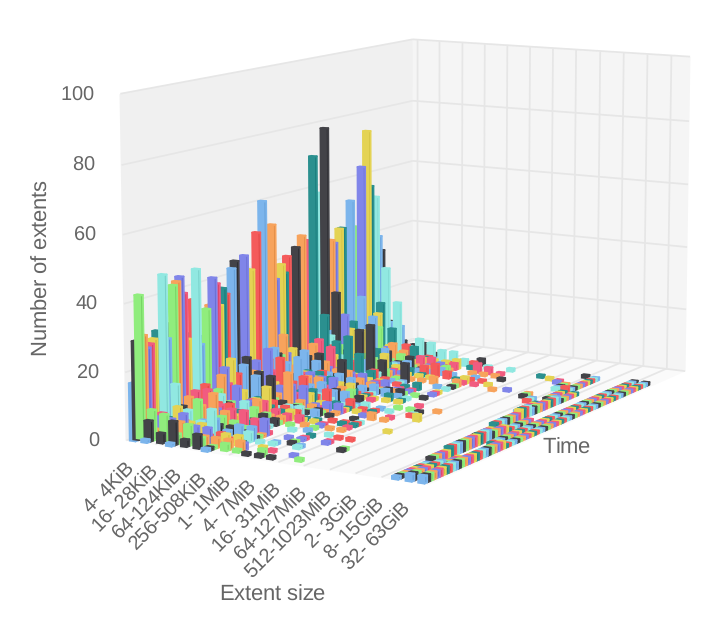
\includegraphics[width=\textwidth]{../charts/HDD_xfs/free80.png}
        \caption[Free space fragmentation of XFS during testing of medium utilisation of HDD]{On this figure we can see tendency of XFS to merge free space blocks into very large extents (up to $\SI{63}{\gibi\byte}$). Furthermore, low fragmentation can be observed during testing time, with quite large blocks of free space even at the end of the test. This chart displays last 7 hours of the test.}
\label{fig:free80_xfs}
\end{figure}


\begin{figure}[!htb]
    \centering
    \fbox{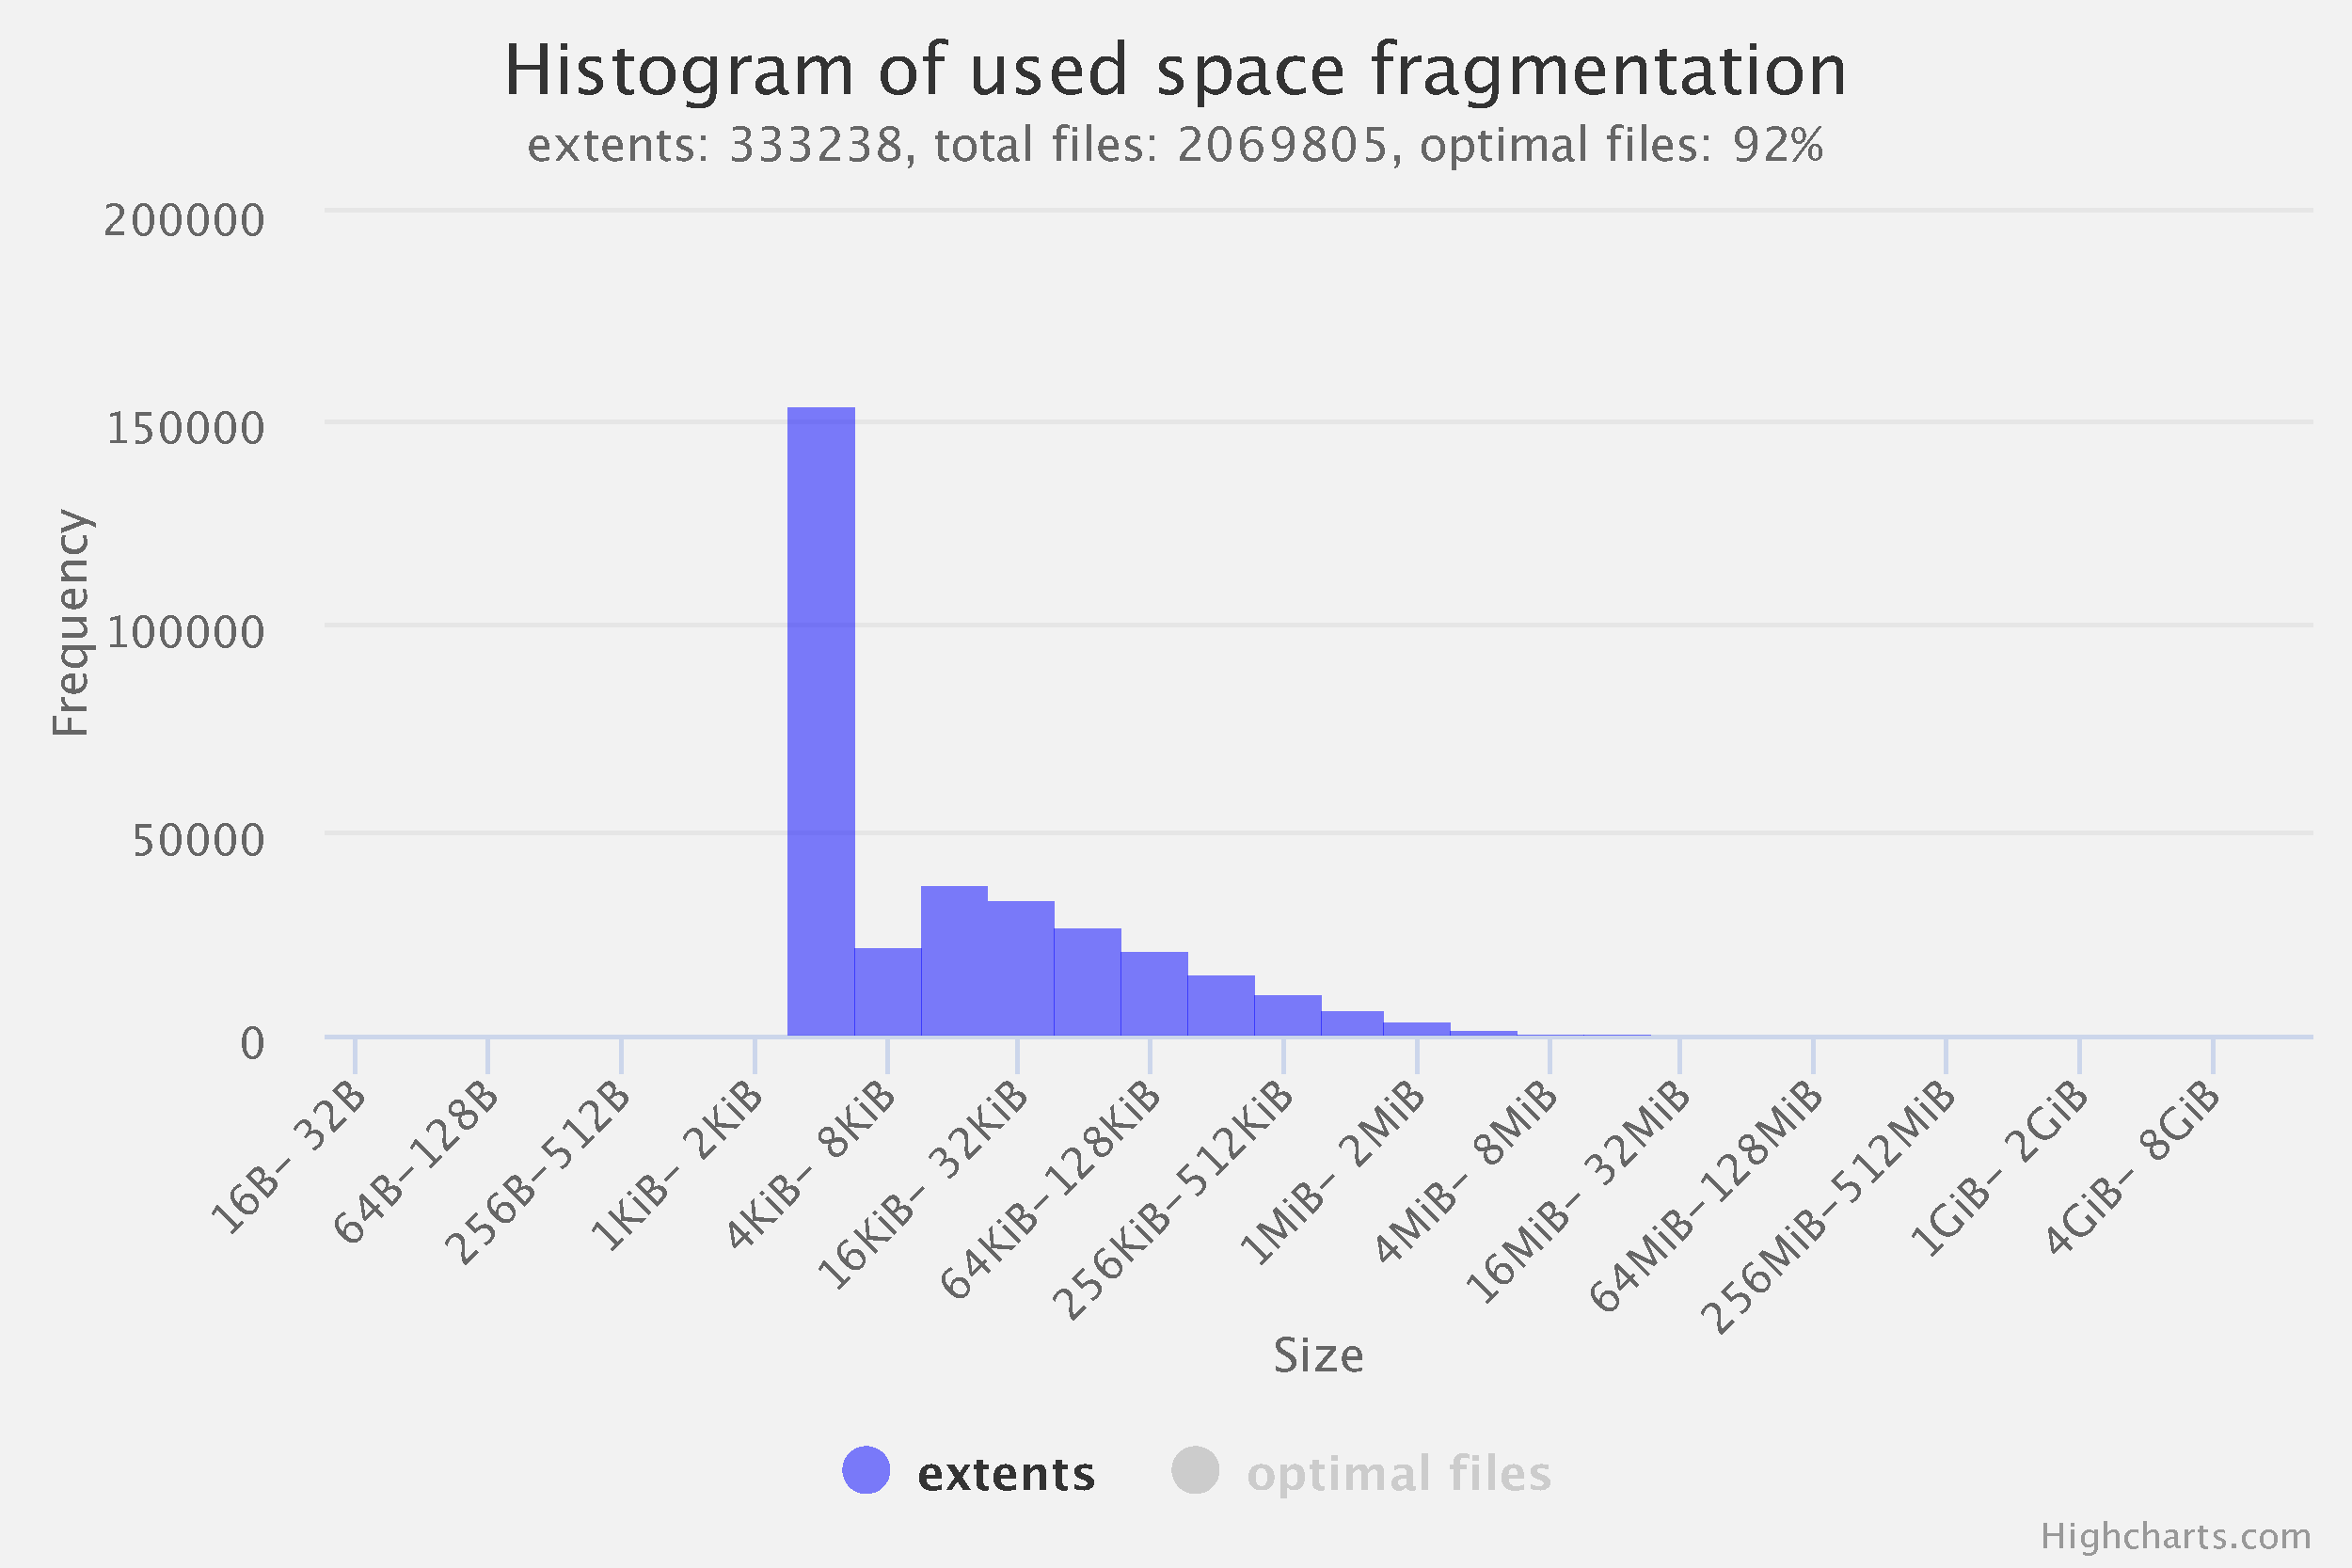
\includegraphics[width=\textwidth,keepaspectratio]{../charts/HDD_xfs/used80}}
    \caption[Size distribution of file extents of XFS during testing of medium utilisation of HDD]{On this chart, we can see that despite low fragmentation of free space, about 333 thousands of file extents were present in the final block layout. However, 92\% of files were still optimally allocated. Furthermore, we can see that most of the created extents are the smallest possible size ($\SI{4}{\kilo\byte}$, i.e. file system block size).}
    \label{fig:used80_xfs}
\end{figure}

\begin{figure}[!htb]
    \begin{minipage}{\textwidth}
        \centering
        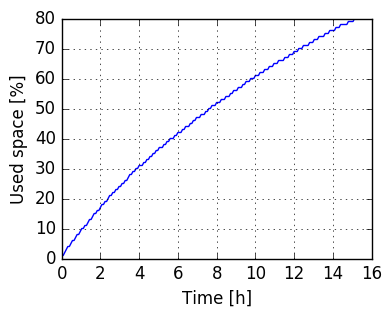
\includegraphics[width=0.7\textwidth]{../charts/HDD_xfs/600.png}
        \caption[Usage of available space of XFS during testing of medium utilisation of HDD]{On this chart, system utilisation over time is displayed. We can see slight curvature of the line, meaning, growth of file system is slowing down. This can be caused by progressively more successful delete operation (with more files, there is greater probability of deleting) and by progressively slower block allocating operations such as create, append and random write.}
\label{fig:usage80_xfs}
    \end{minipage}
\end{figure}


\begin{figure}[!htb]
    \centering
   \begin{minipage}{\textwidth}
        \centering
        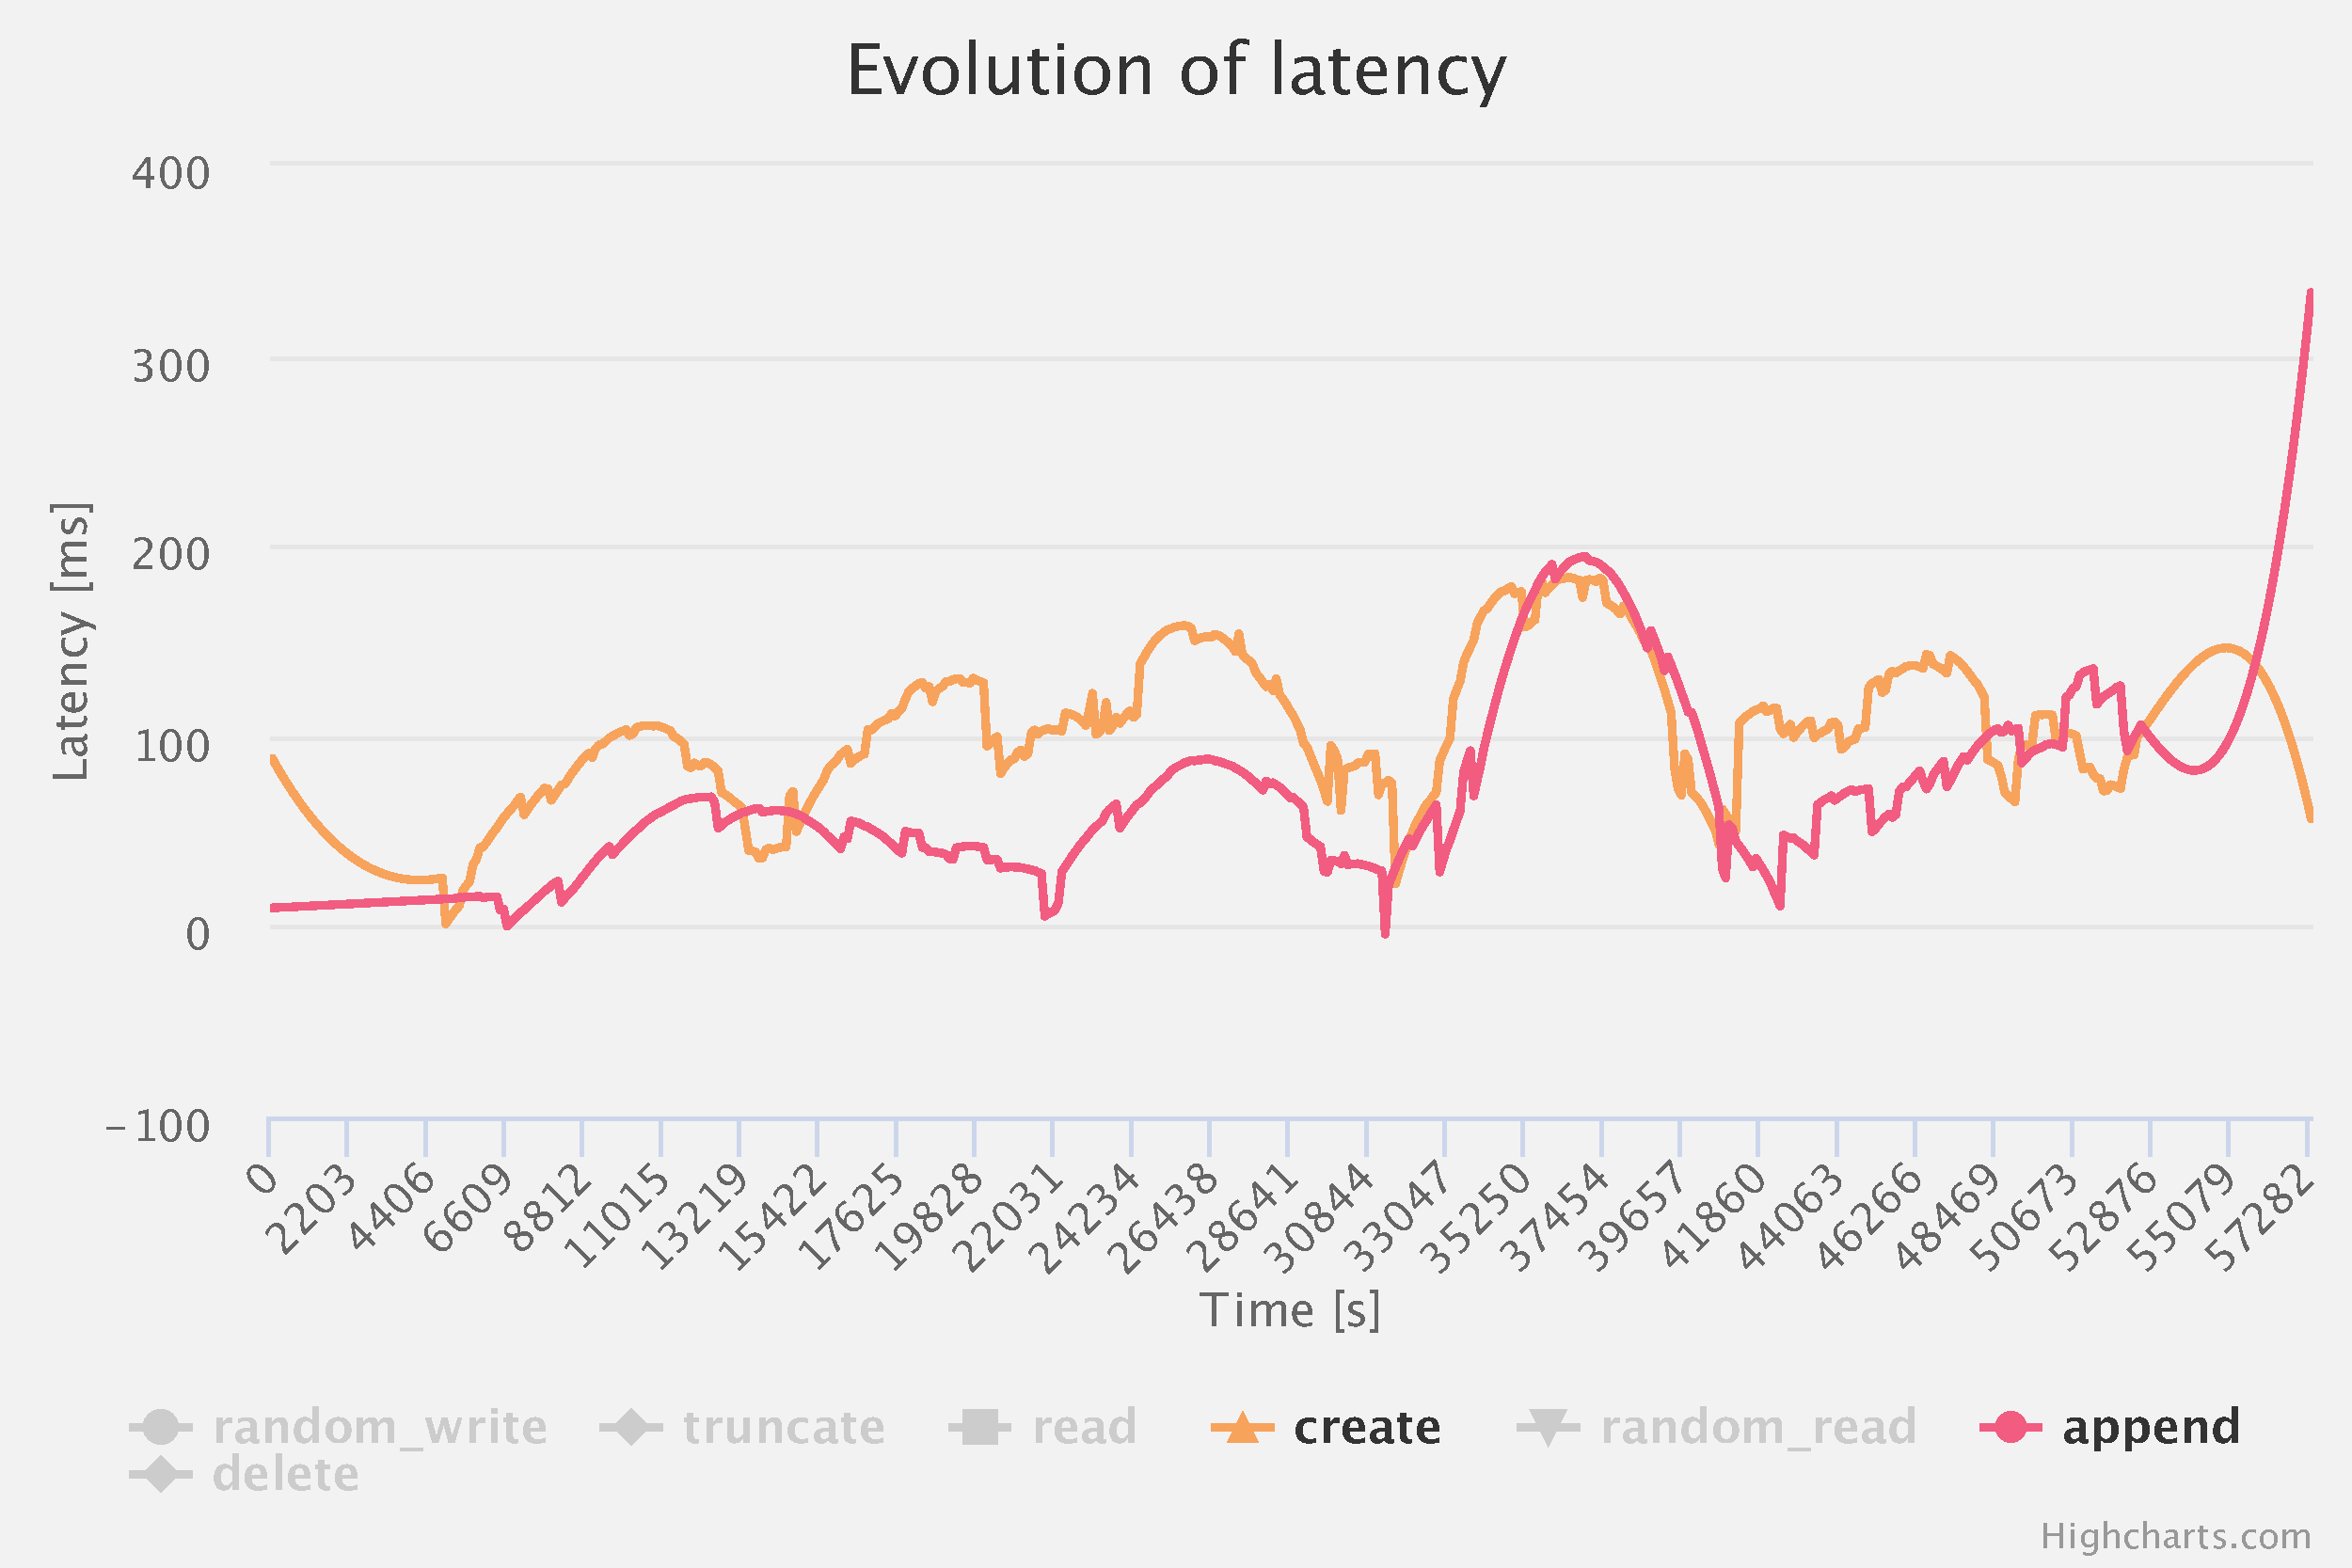
\includegraphics[width=\textwidth]{../charts/HDD_xfs/low_ca}
        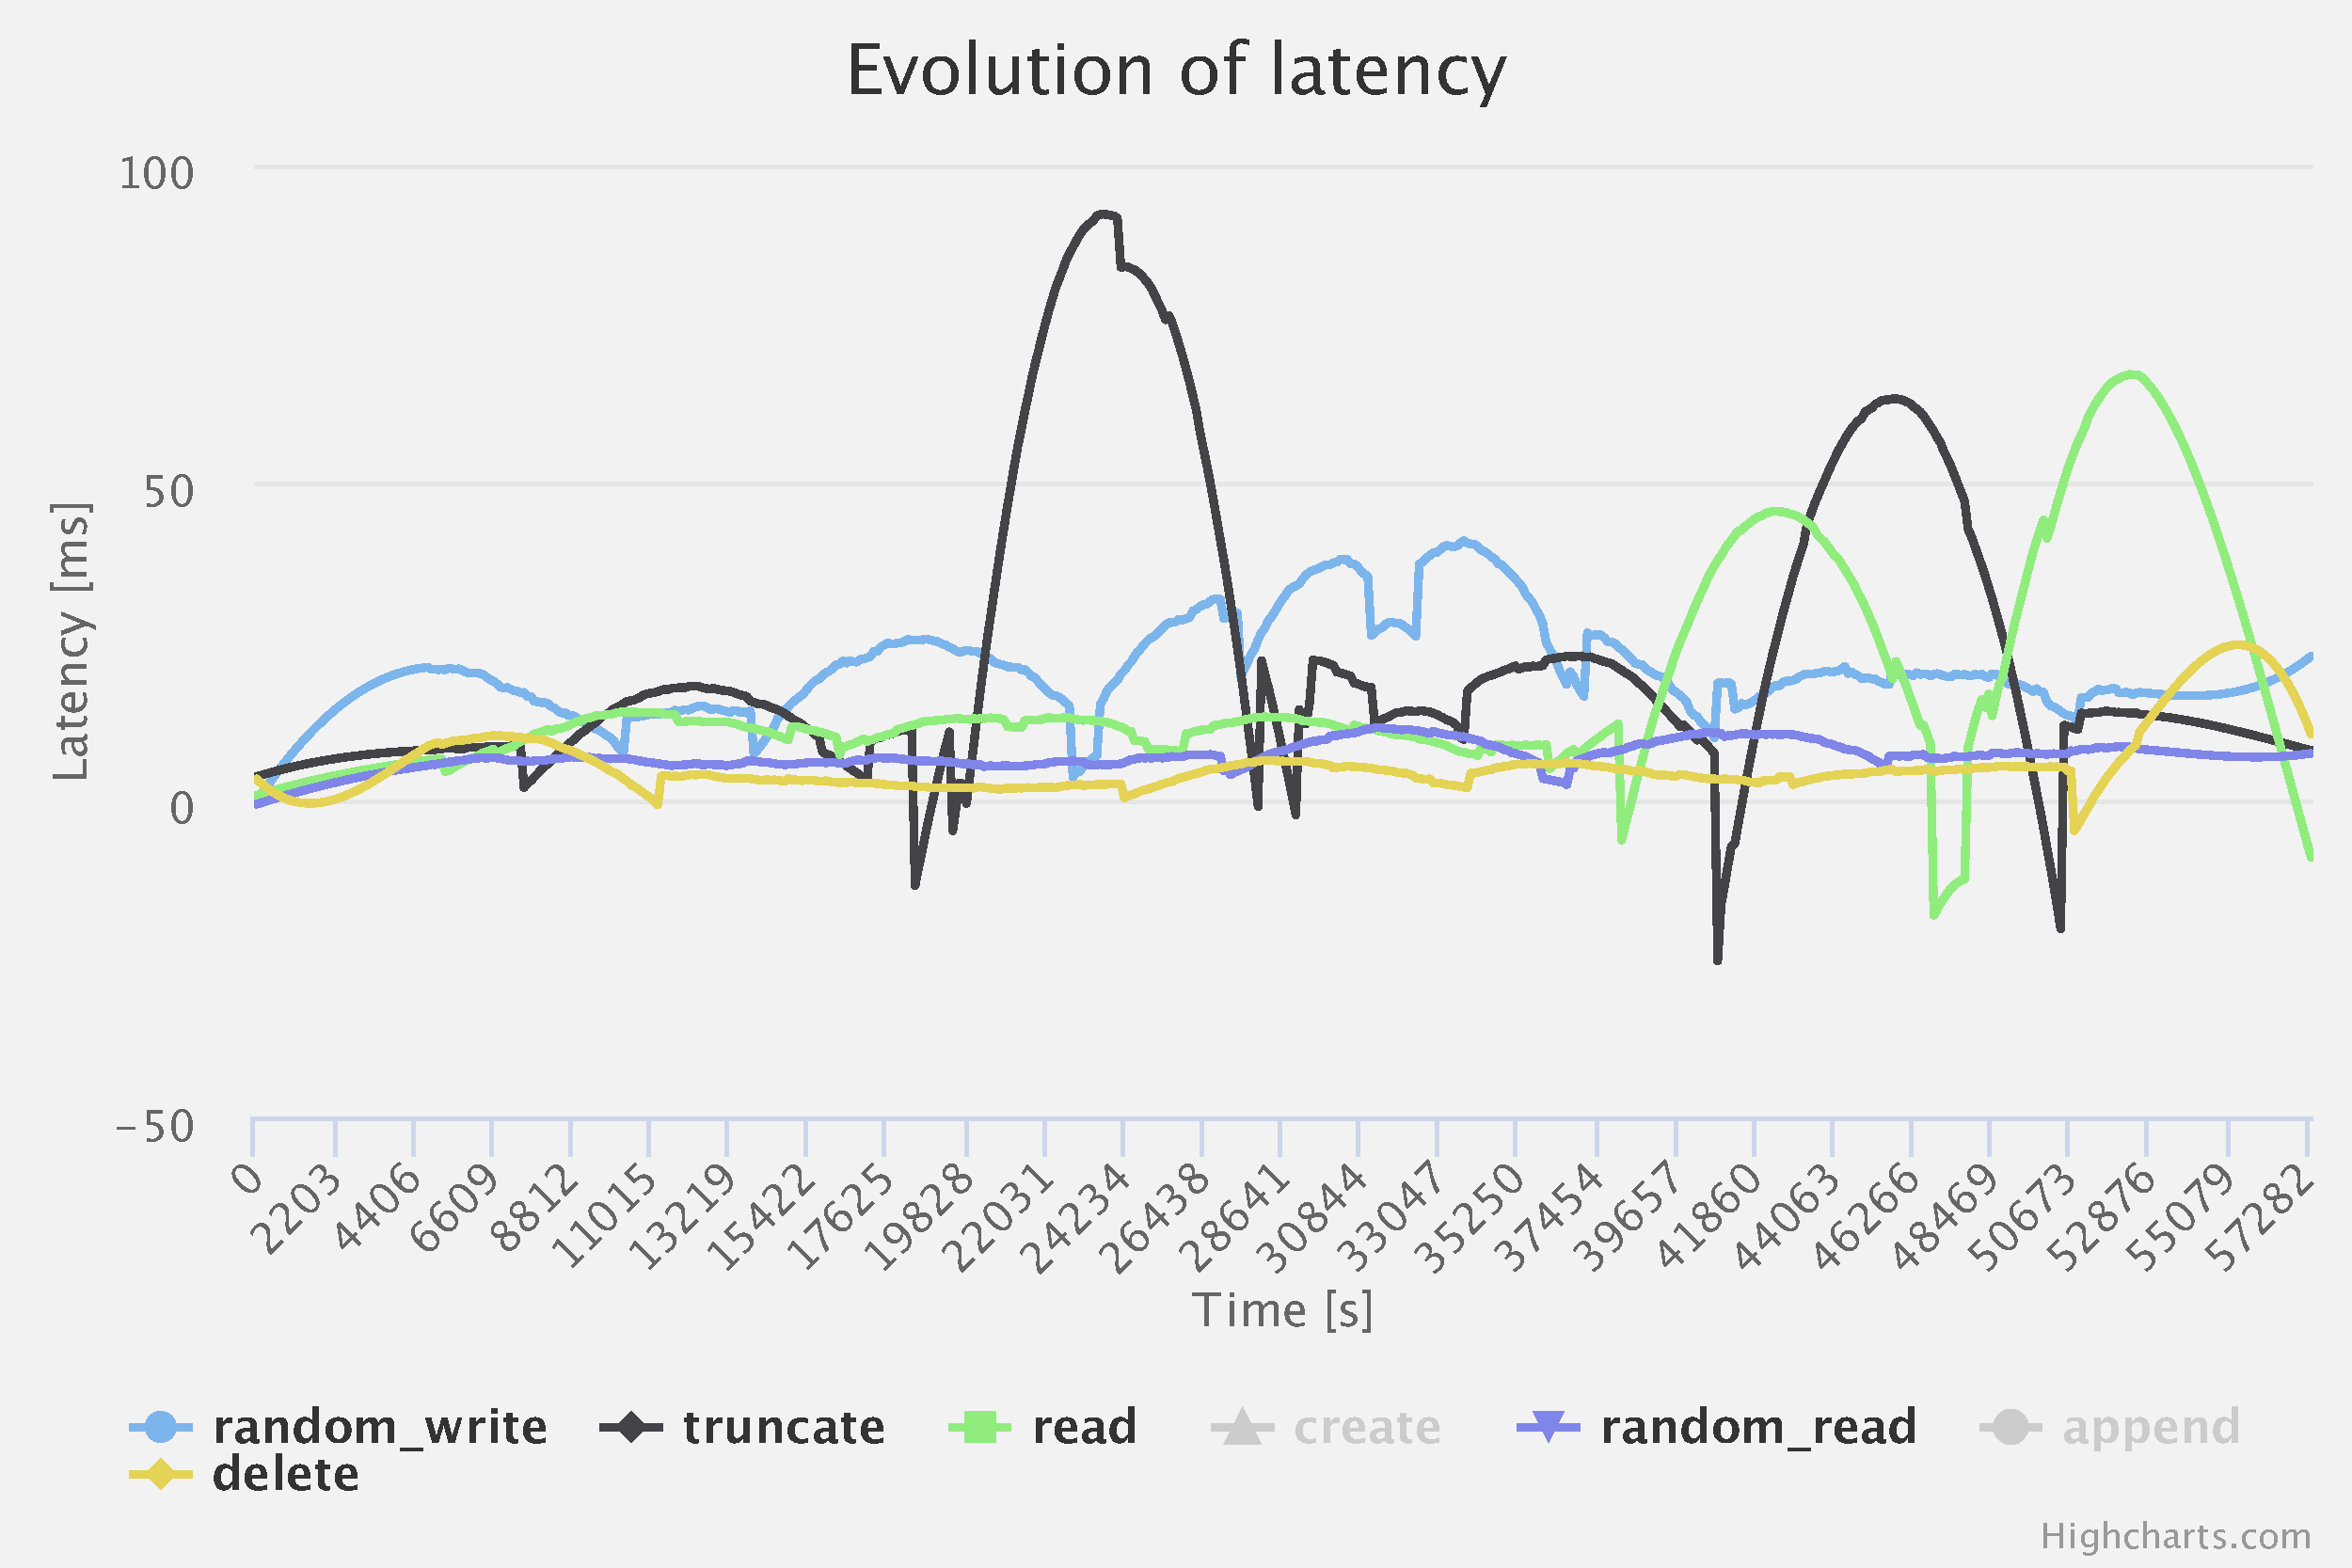
\includegraphics[width=\textwidth]{../charts/HDD_xfs/low_others}
        \caption[Evolution of latencies of XFS during testing of medium utilisation of HDD]{Evolution of latencies of conducted IO operations during testing XFS with medium utilisation. Progressively larger fluctuations can be seen in sequential read. Latency of operation append seems to be slowly raising in the last hour of the test.}
\label{fig:lats80_xfs}
    \end{minipage}
\end{figure}

\clearpage

\section{Test of high utilisation using XFS on HDD}
\begin{itemize}
\itemsep0em 
   \item System: Machine\,3
   \item OS: RHEL-7.3
   \item Kernel: 3.10.0-514.el7.x86\_64
\end{itemize}

\begin{figure}[h]
    \centering
    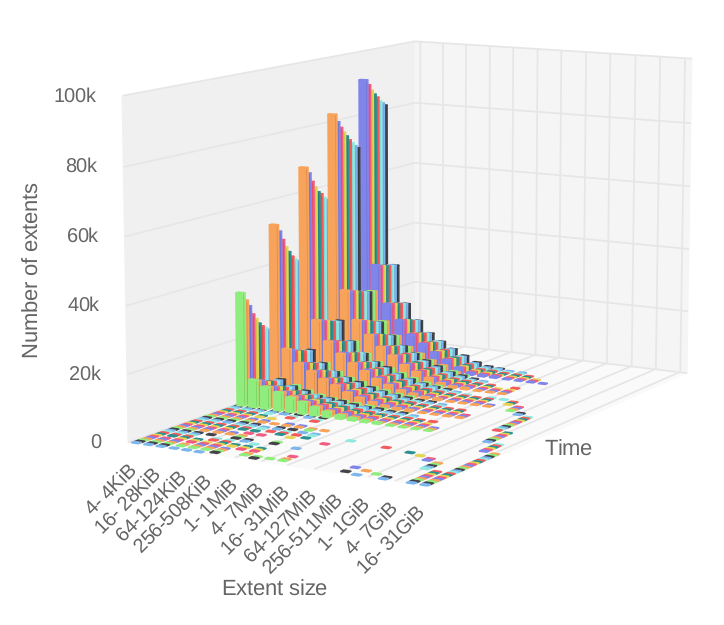
\includegraphics[width=\textwidth,keepaspectratio]{../charts/HDD_xfs/free99.png}
    \caption[Evolution of free space fragmentation of XFS during testing of high utilisation of HDD]{On this chart, we can see evolution of free space fragmentation in the last 5 hours of the test. When comparing this chart with Figure~\ref{fig:usage99_xfs}, we can see that peak in number of extents always appear when the test is randomly deleting space. After that, XFS tries to merge small free space extents into larger ones and successfully defragments free space.}
    \label{fig:free99_xfs}
\end{figure}

\begin{figure}[h]
    \centering
    \fbox{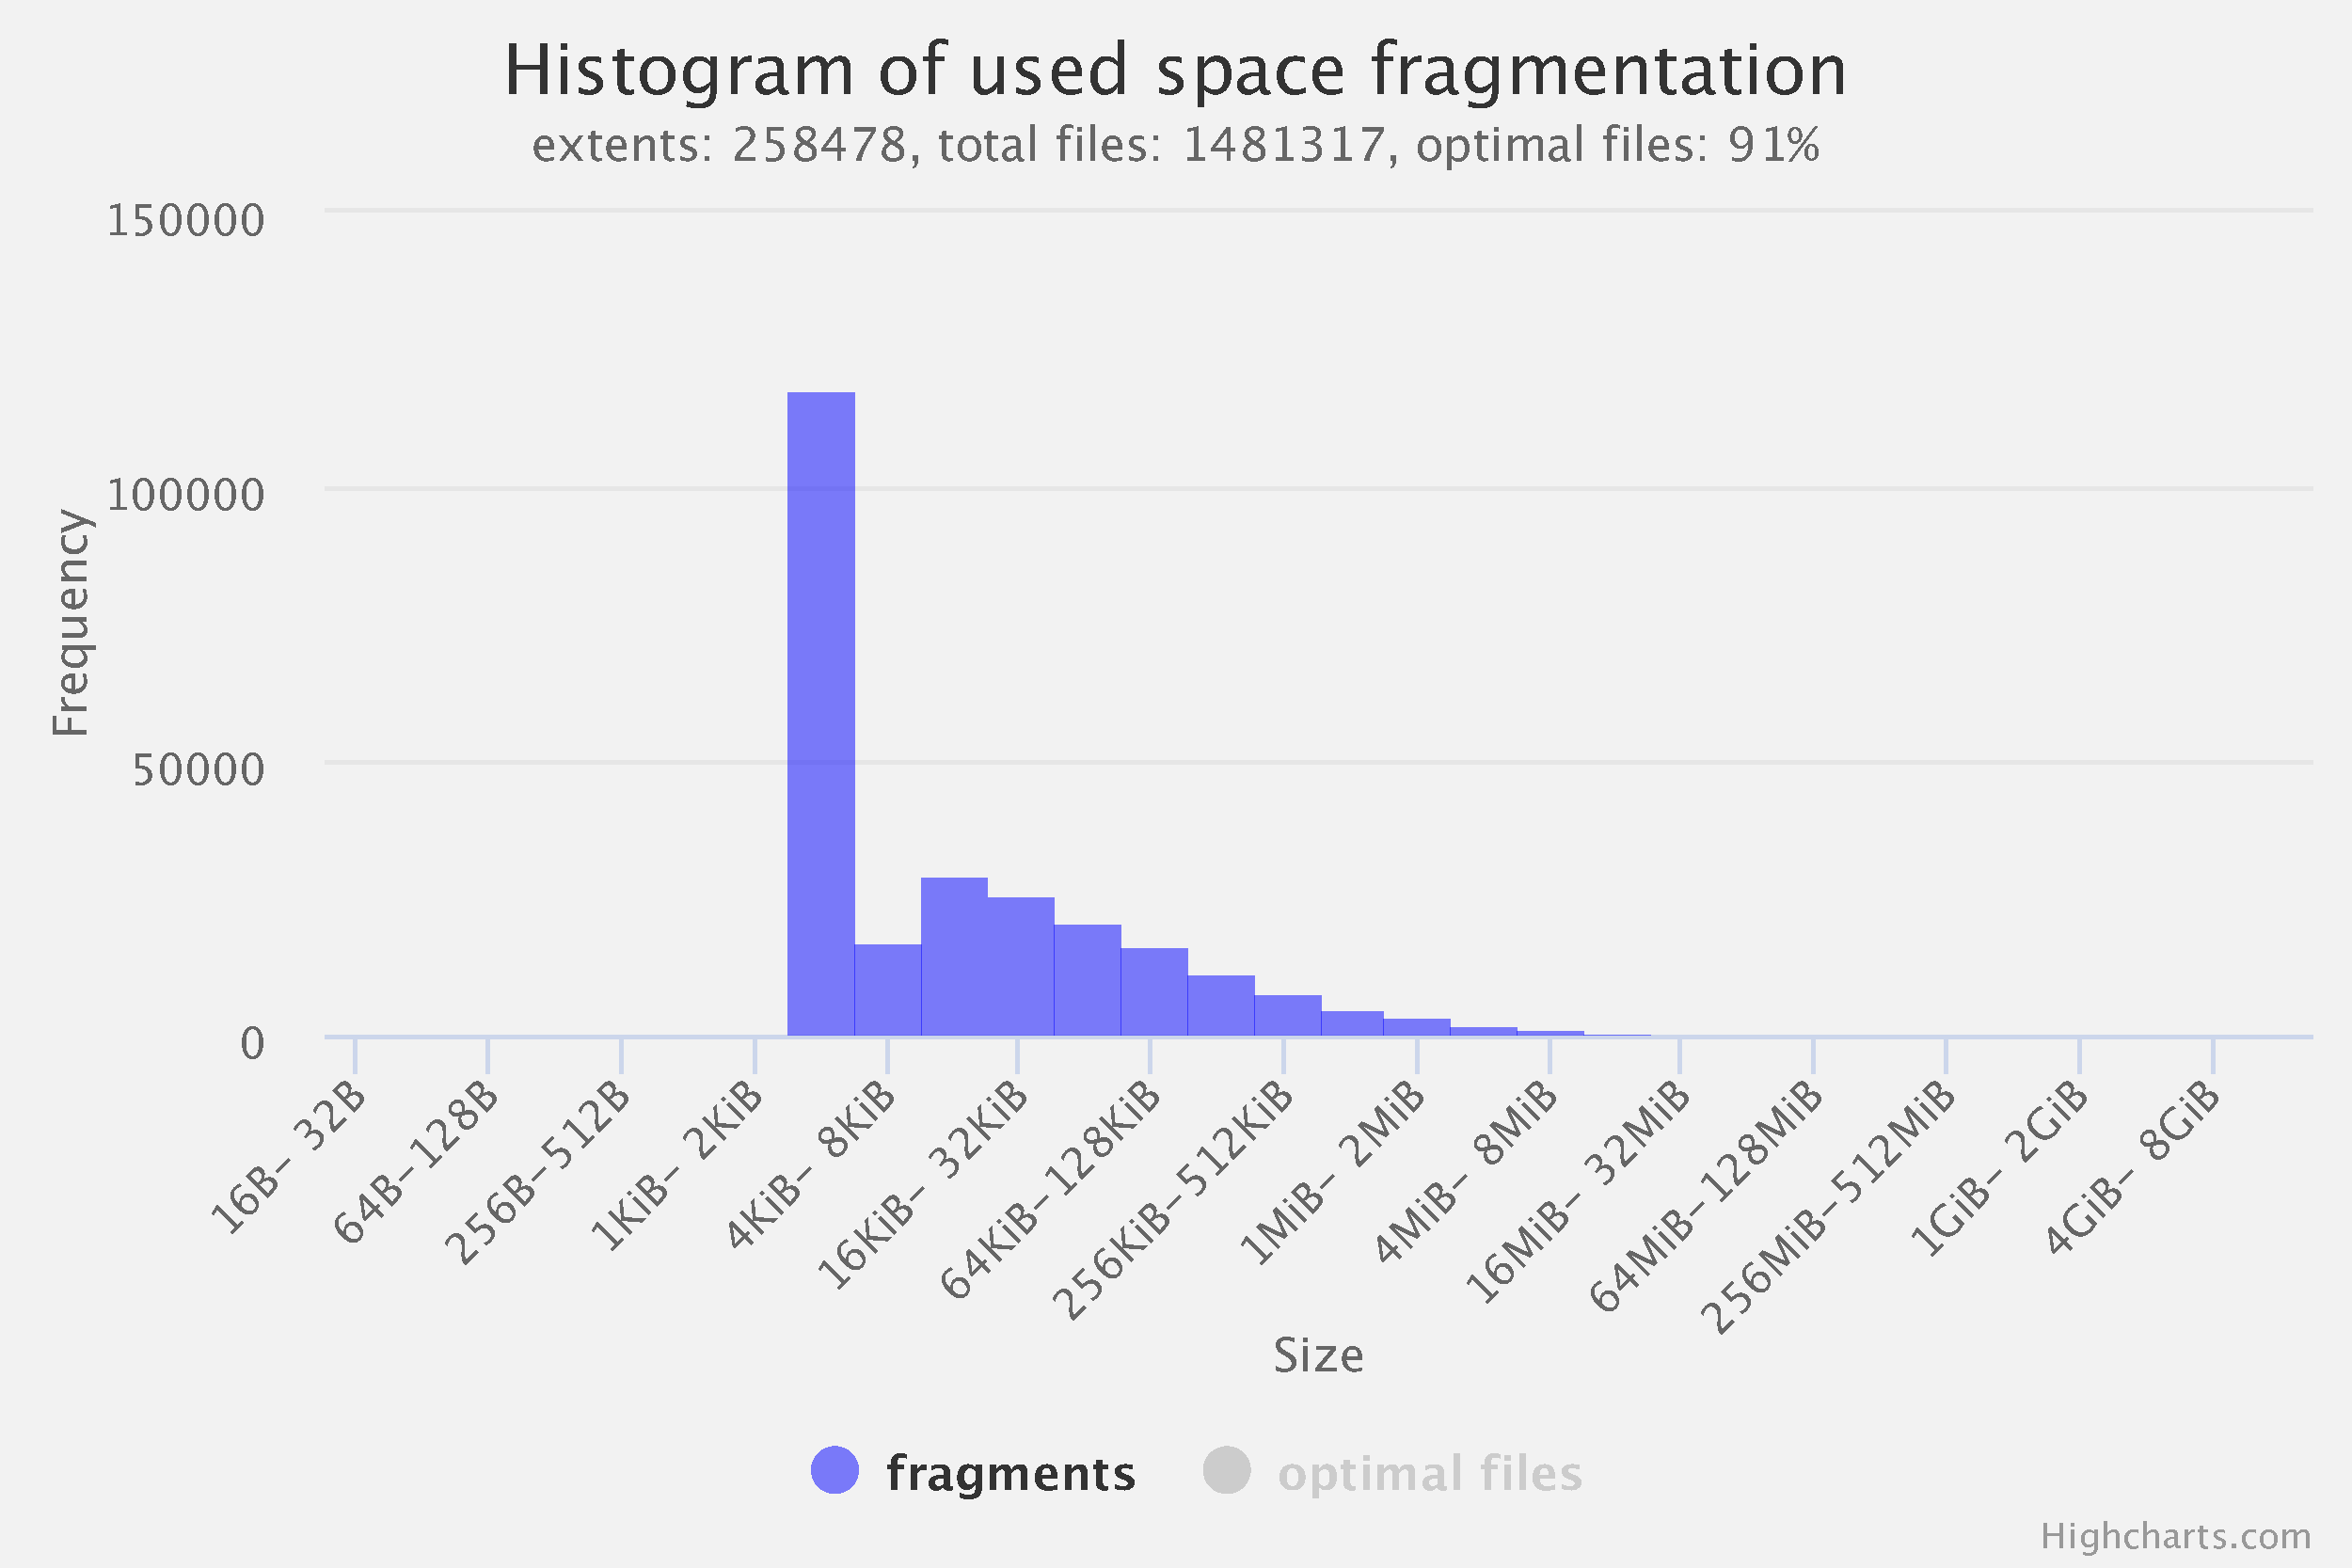
\includegraphics[width=\textwidth,keepaspectratio]{../charts/HDD_xfs/used99}}
    \caption[Size distribution of file extents of XFS during testing high utilisation of HDD]{On this chart, we can see that despite high fragmentation of free space, 91\% of files were optimally allocated. Distribution of extents of used space is similar to distribution observed while testing with medium utilisation.}
    \label{fig:used99_xfs}
\end{figure}

\begin{figure}[!h]
    \begin{minipage}{\textwidth}
        \centering
        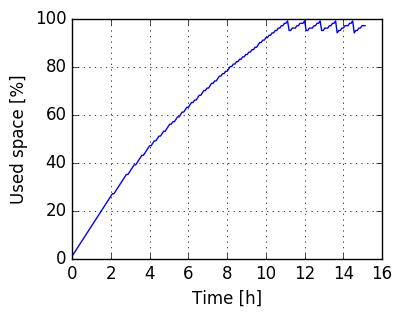
\includegraphics[width=0.7\textwidth]{../charts/HDD_xfs/300.png}
        \caption[Usage of available space of XFS during testing of high utilisation of HDD]{File system utilisation over time. We can see that deletion of used space was triggered five times. It took the test approximately 10.5 hours to fill available space ($\SI{300}{\giga\byte}$).}
\label{fig:usage99_xfs}
    \end{minipage}
\end{figure}

\begin{figure}[!htb]
    \centering
   \begin{minipage}{\textwidth}
        \centering
        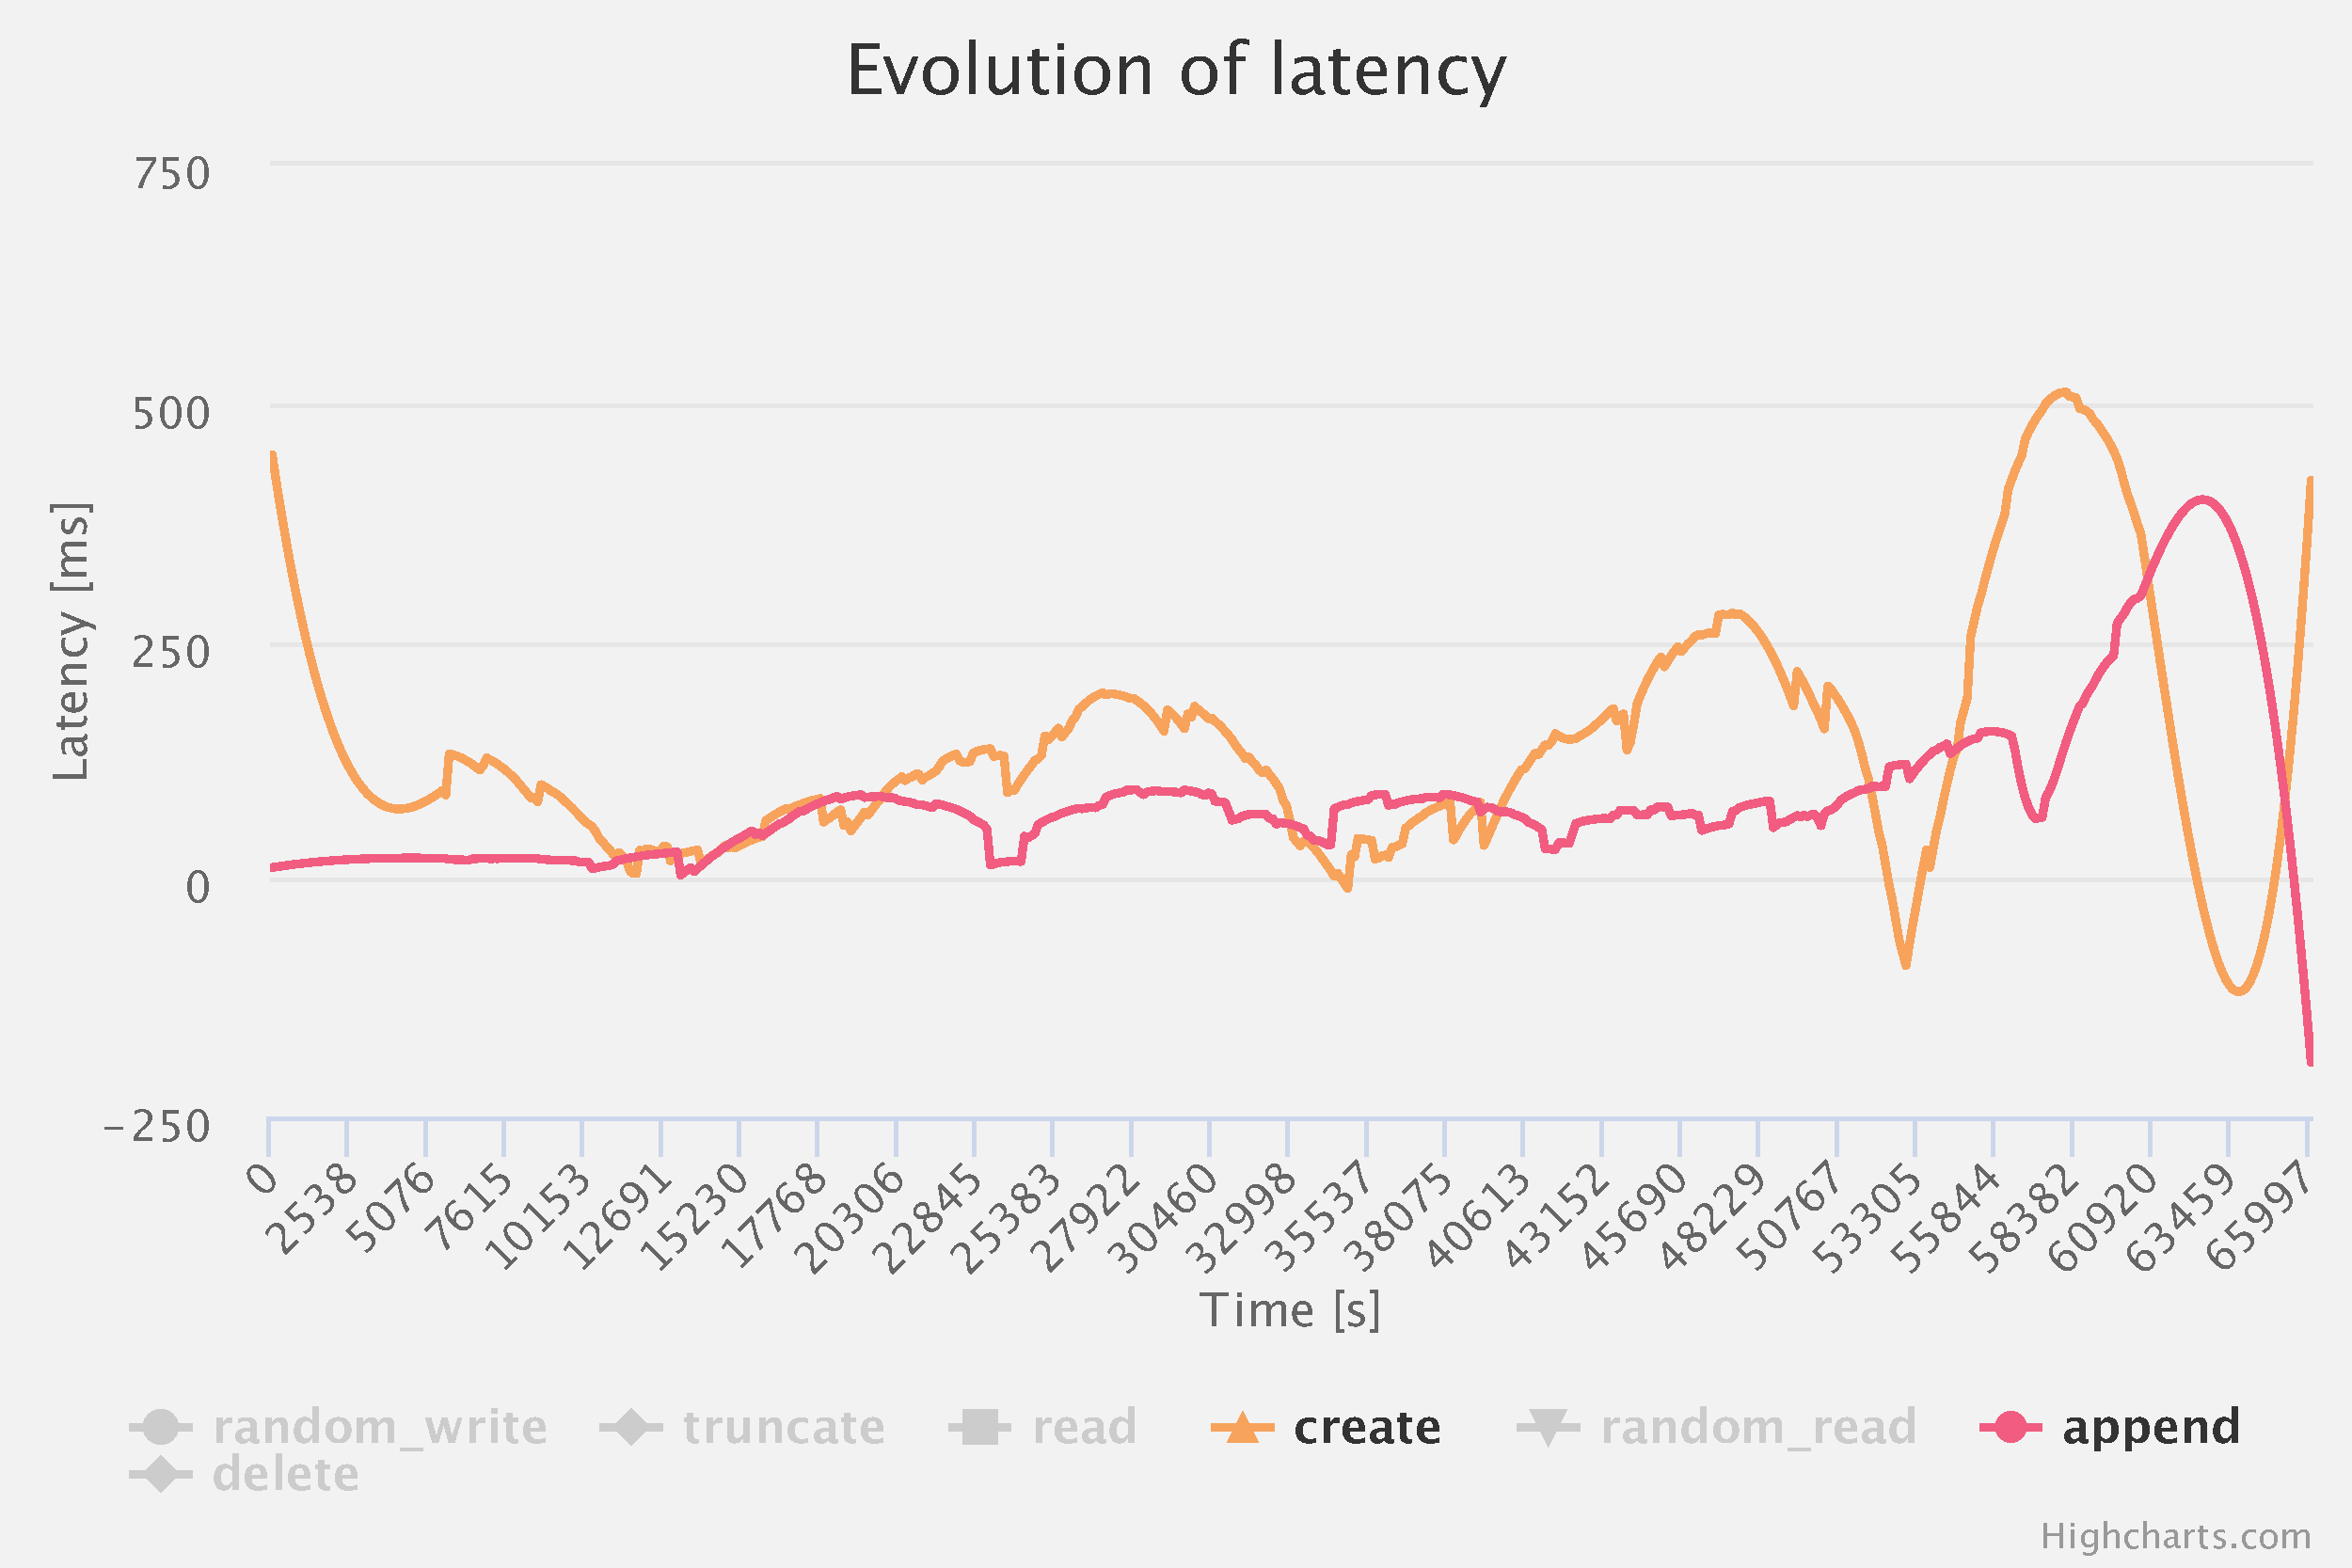
\includegraphics[width=\textwidth]{../charts/HDD_xfs/high_ca}
        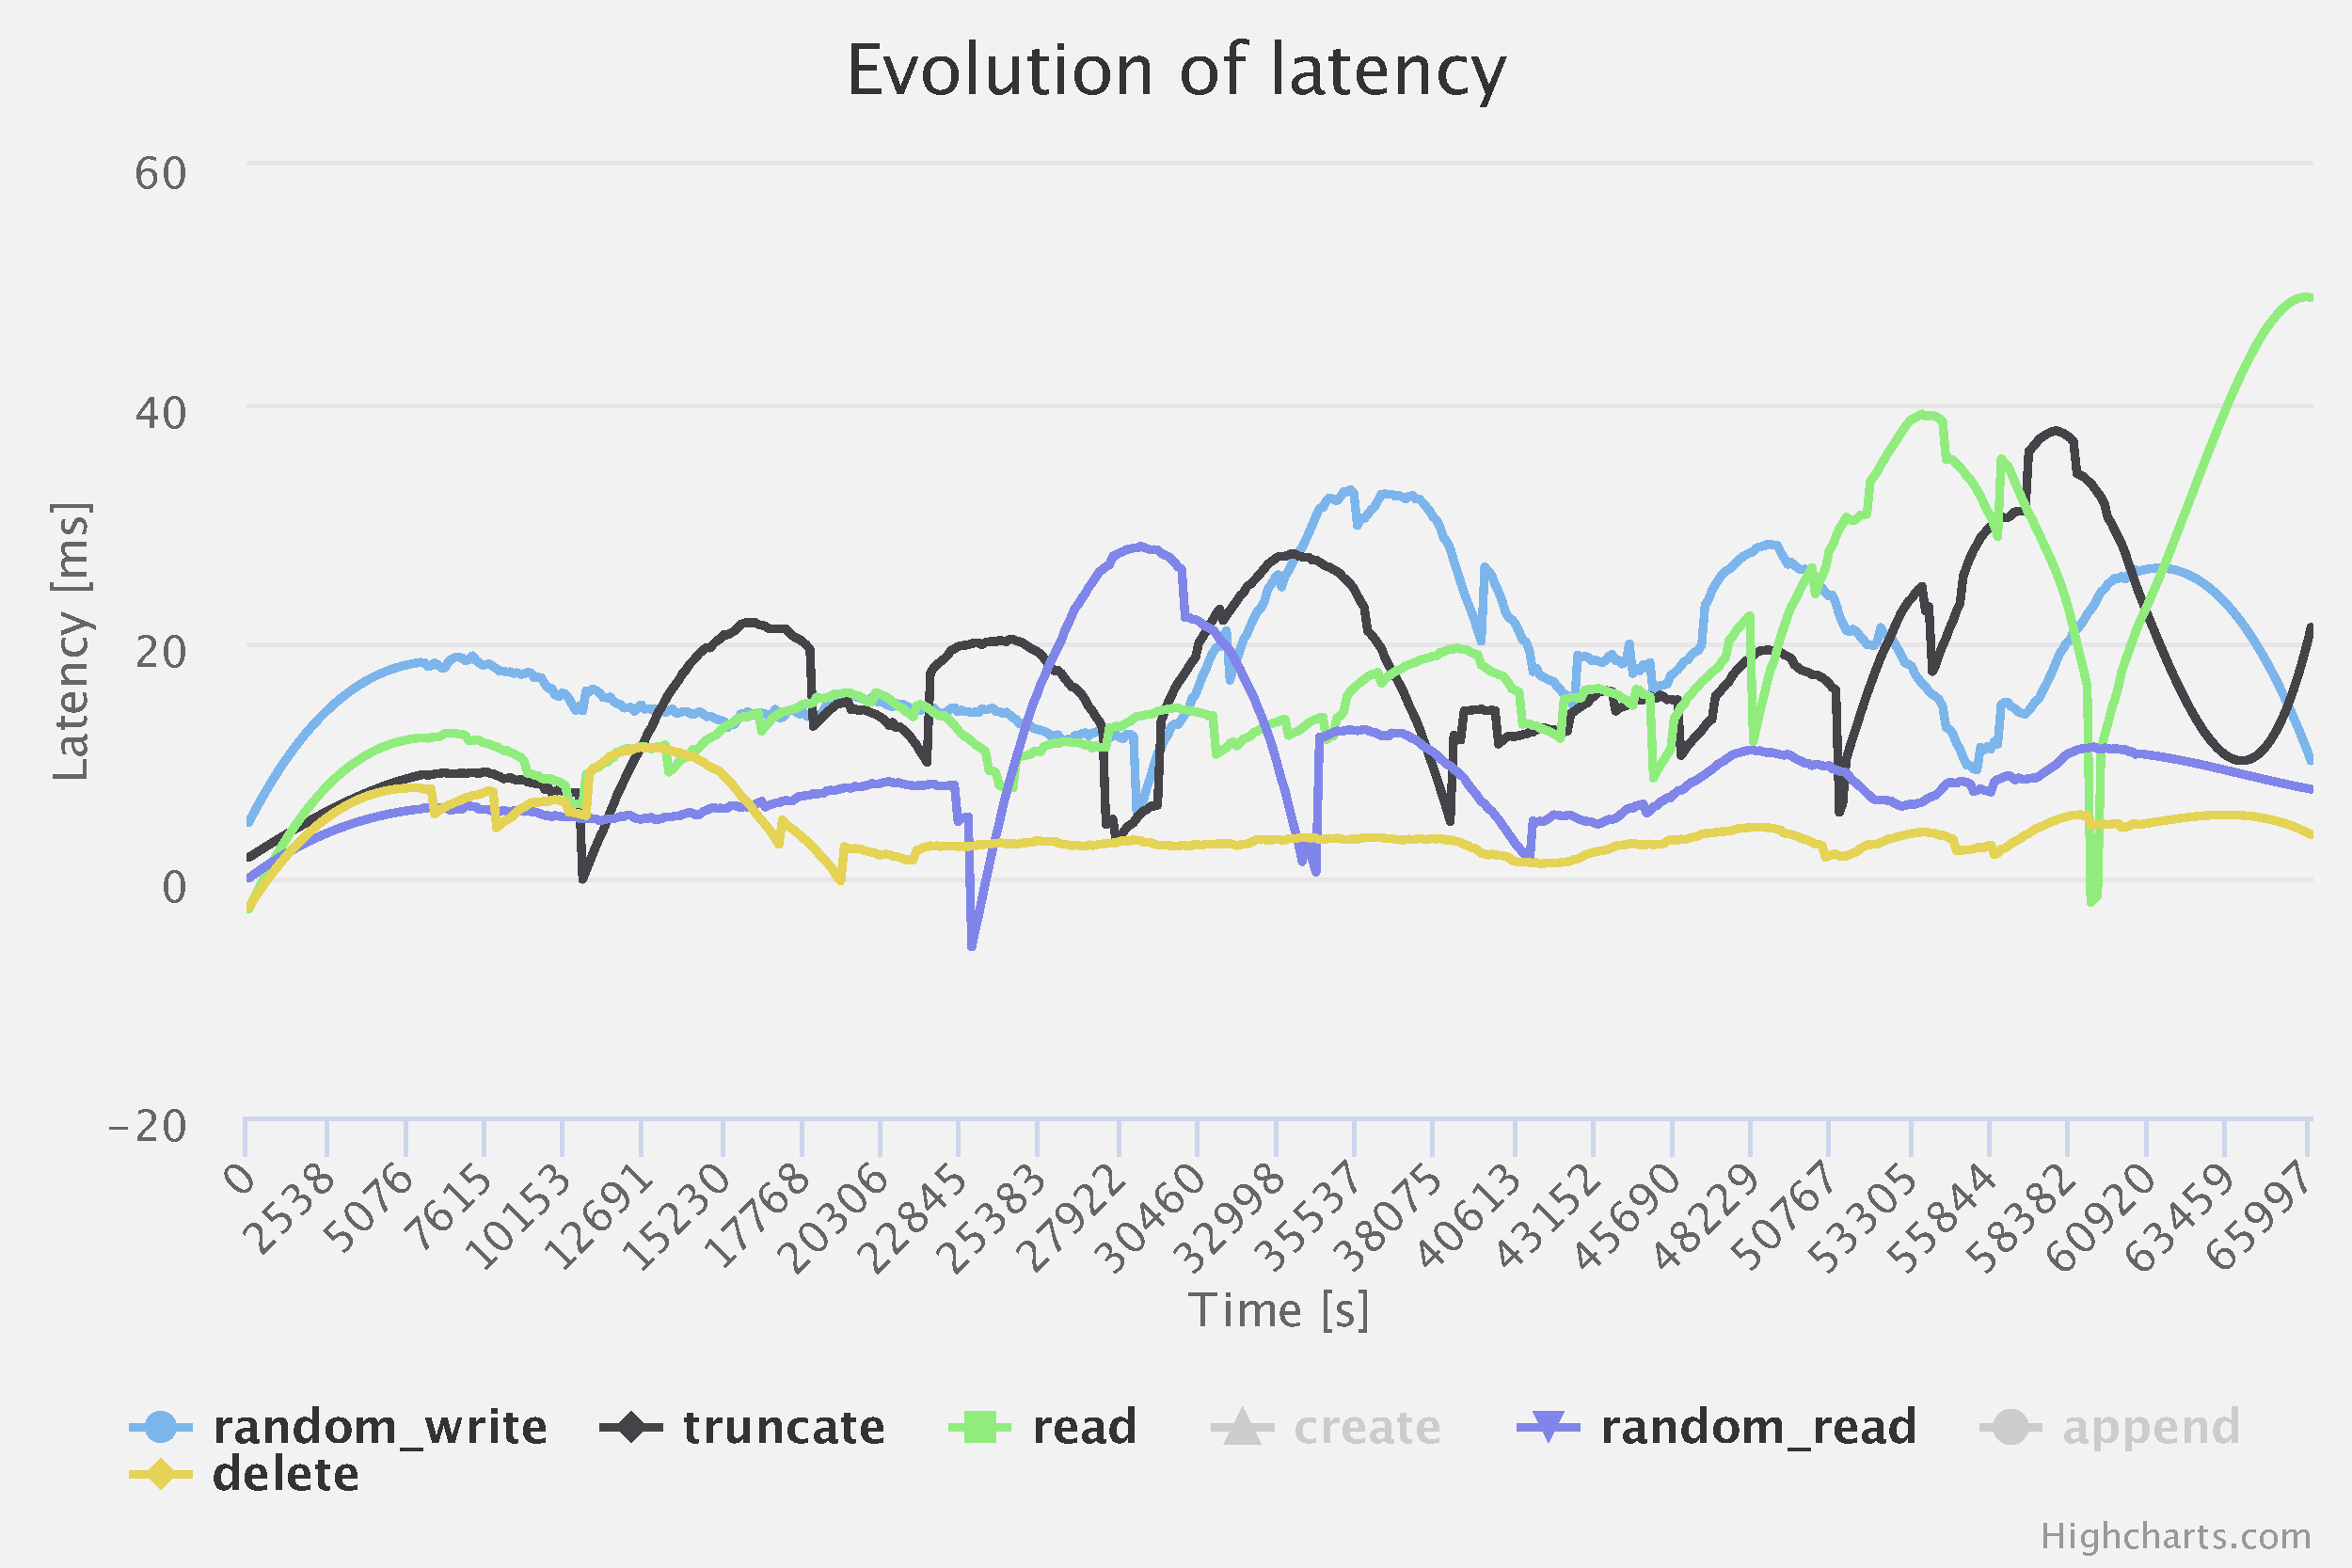
\includegraphics[width=\textwidth]{../charts/HDD_xfs/high_other}
        \caption[Evolution of latencies of XFS during testing of high utilisation of HDD]{Evolution of latencies of IO operations during testing XFS with high utilisation. Progressively larger fluctuations can be seen in create and append operations. Some other operations such as sequential read of truncate are showing progressive growth, mainly after file system reached highest utilisation.}
\label{fig:lats99_xfs}
    \end{minipage}
\end{figure}


\clearpage


\section{Test of high utilisation using ext4 on HDD}
\begin{itemize}
\itemsep0em 
   \item System: Machine\,3
   \item OS: RHEL-7.3
   \item Kernel: 3.10.0-514.el7.x86\_64
\end{itemize}

\begin{figure}[h]
    \centering
    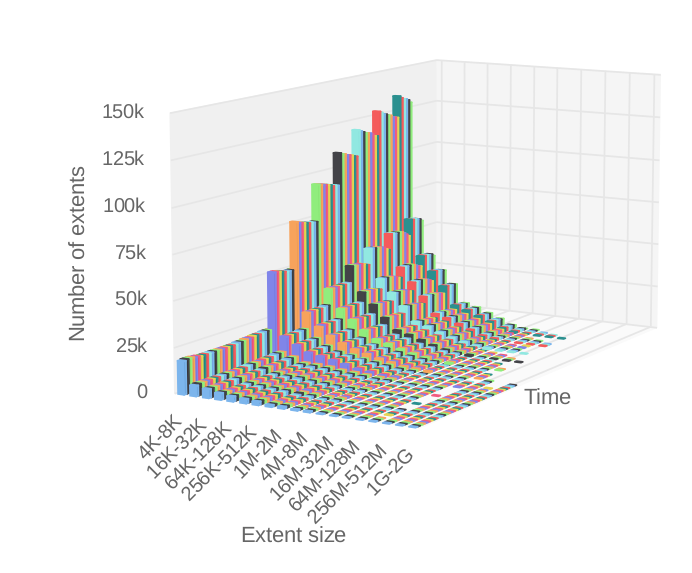
\includegraphics[width=\textwidth,keepaspectratio]{../charts/HDD_ext4/free.png}
    \caption[Evolution of free space fragmentation of ext4 during testing of high utilisation of HDD]{This chart shows evolution of free space fragmentation in the last 5 hours of the test. When comparing this chart with Figure~\ref{fig:usage99_ext4}, we can see that peak in number of extents always appear when the test is randomly deleting space. After that, ext4 fails to merge small free space extents into larger ones as effectively as it could have been observed in XFS.}
    \label{fig:free99_ext4}
\end{figure}

\begin{figure}[h]
    \centering
    \fbox{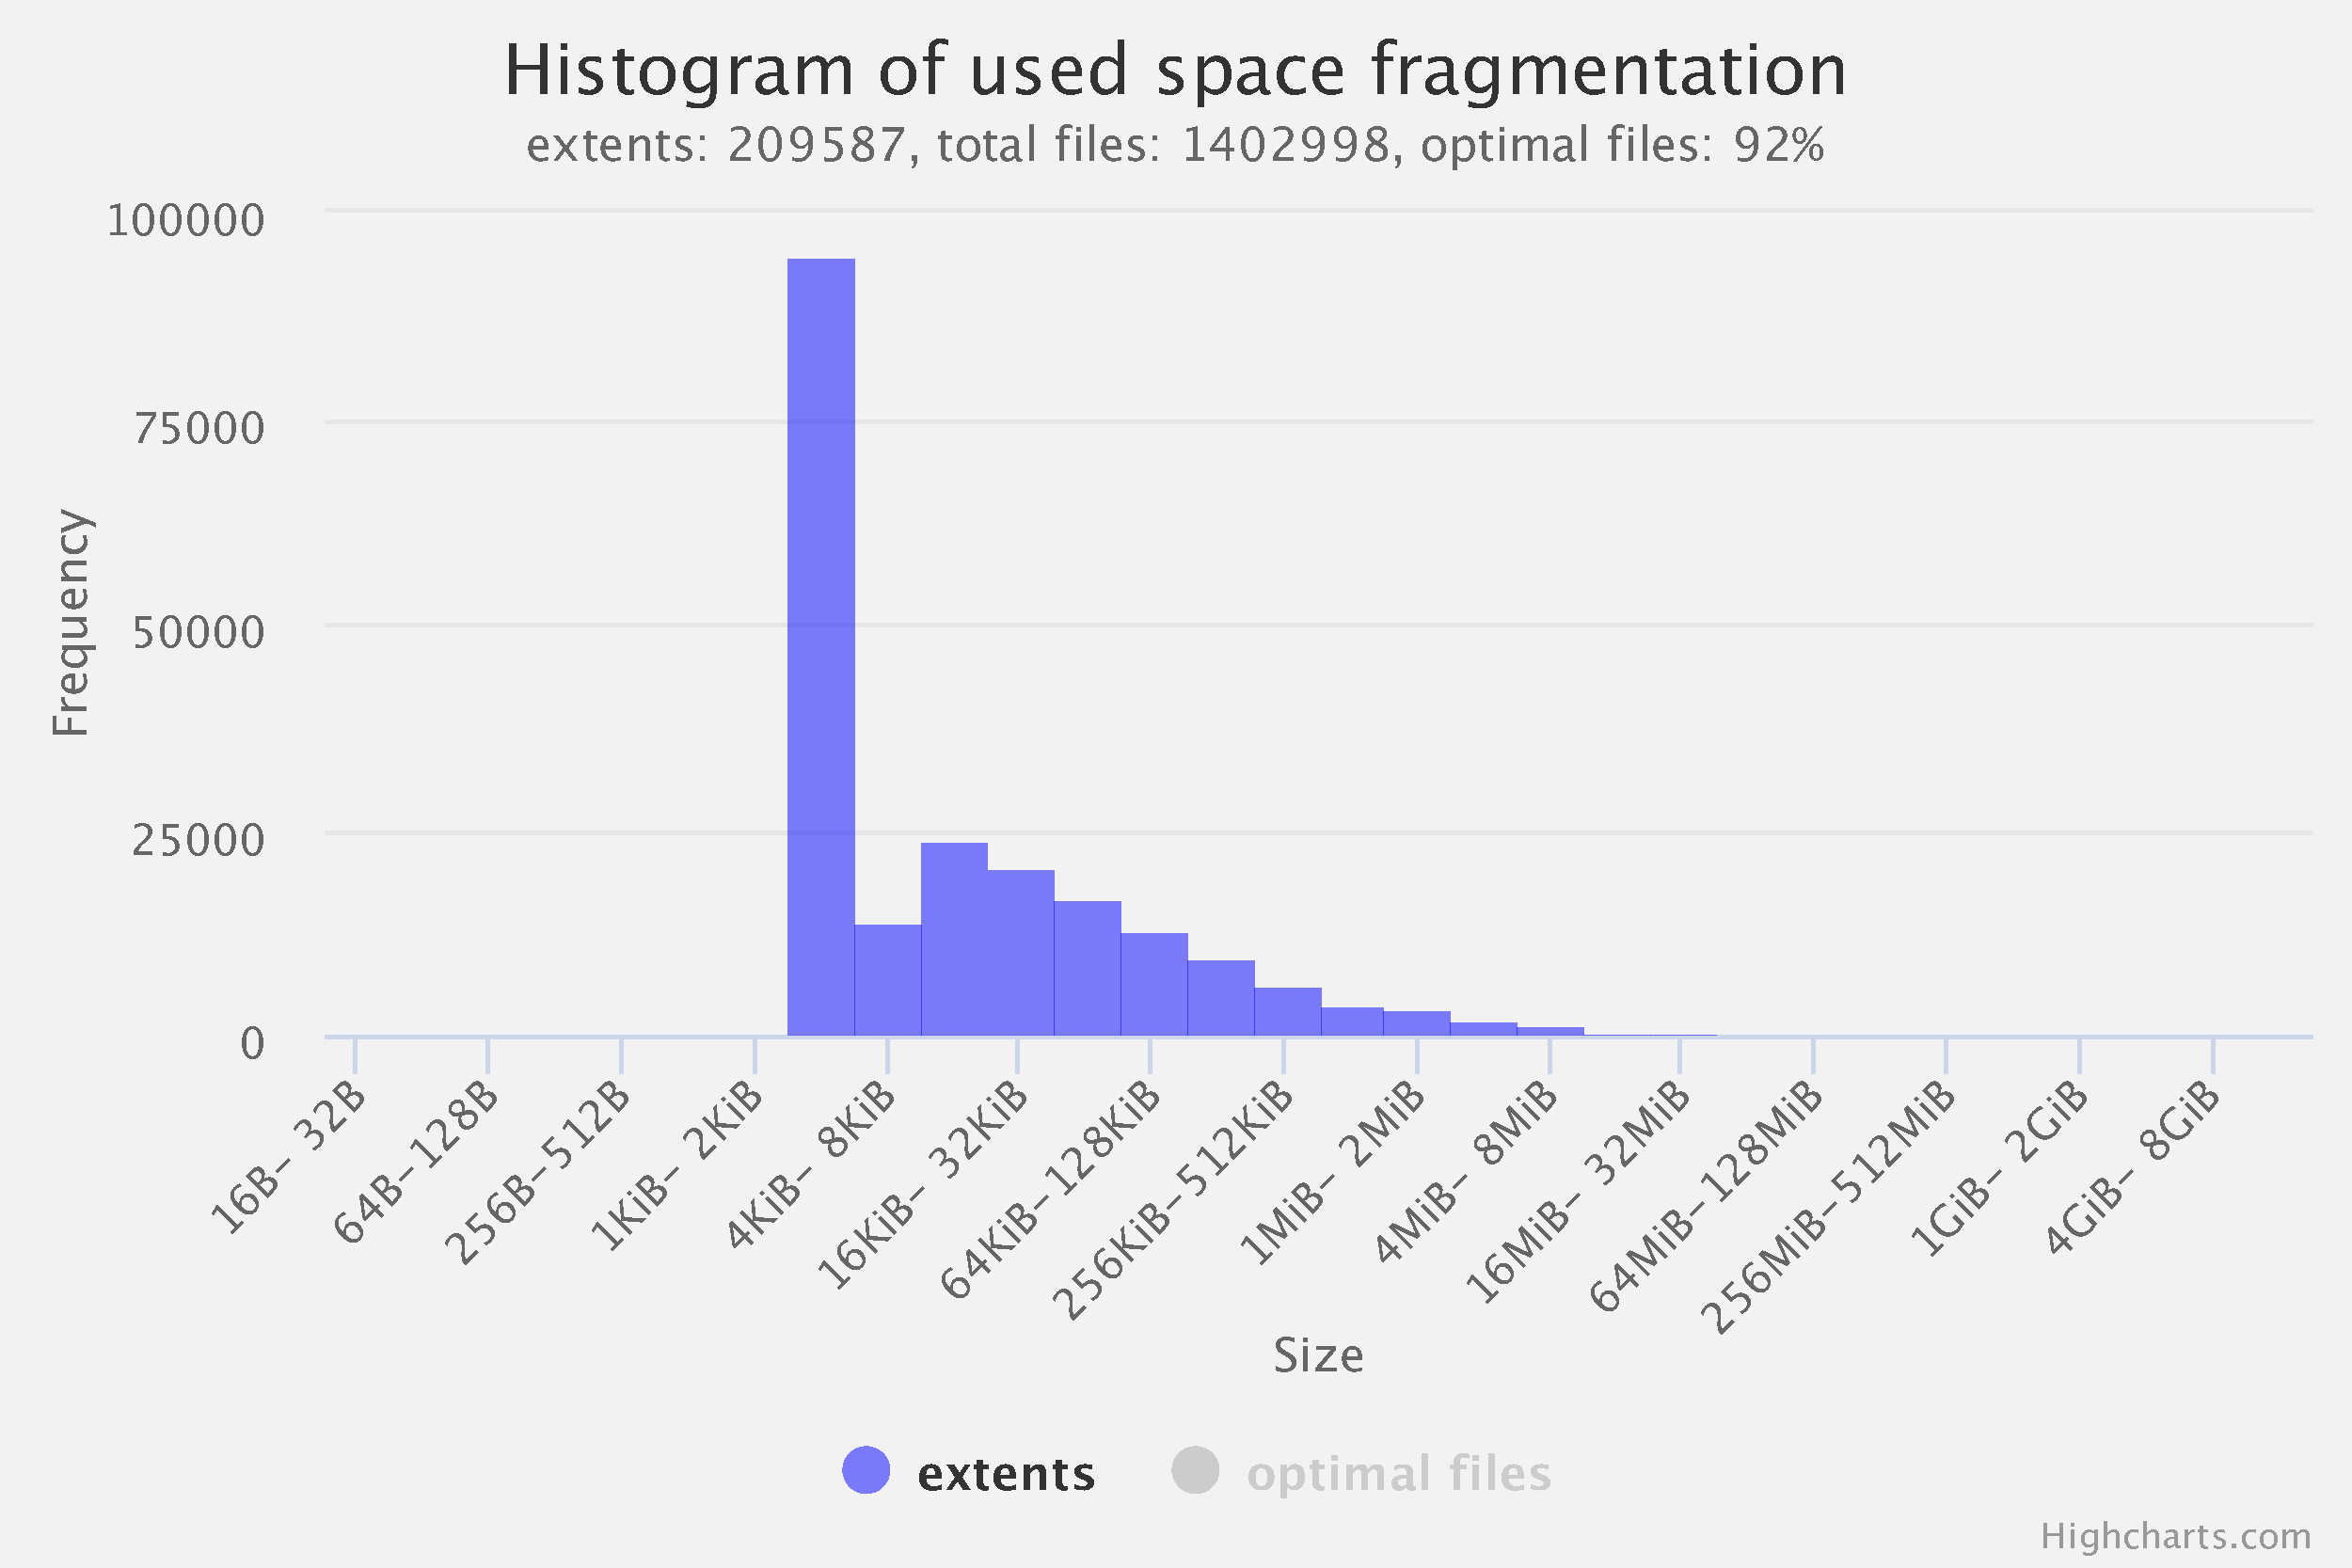
\includegraphics[width=\textwidth,keepaspectratio]{../charts/HDD_ext4/used}}
    \caption[Size distribution of file extents of ext4 during testing of high utilisation of HDD]{On this chart, we can see distribution of size of file extents. Despite high fragmentation of free space during the test, the final block layout of file system have around 274 thousands of extents. 91\% of files were optimally allocated. Furthermore, we can see that most of the created extents are the smallest possible size ($\SI{4}{\kilo\byte}$, i.e. file system block size).}
    \label{fig:used99_ext4}
\end{figure}

\begin{figure}[!h]
    \begin{minipage}{\textwidth}
        \centering
        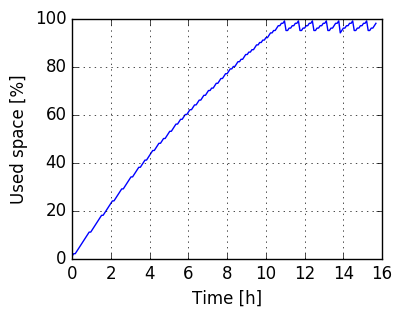
\includegraphics[width=0.7\textwidth]{../charts/HDD_ext4/usage.png}
        \caption[Usage of available space of ext4 during testing of high utilisation of HDD]{Chart displays file system utilisation over time. We can see that deletion of used space was triggered 7 times. It took the test approximately 10.5 hours to fill available space ($\SI{300}{\giga\byte}$).}
\label{fig:usage99_ext4}
    \end{minipage}
\end{figure}

\begin{figure}[!htb]
    \centering
   \begin{minipage}{\textwidth}
        \centering
        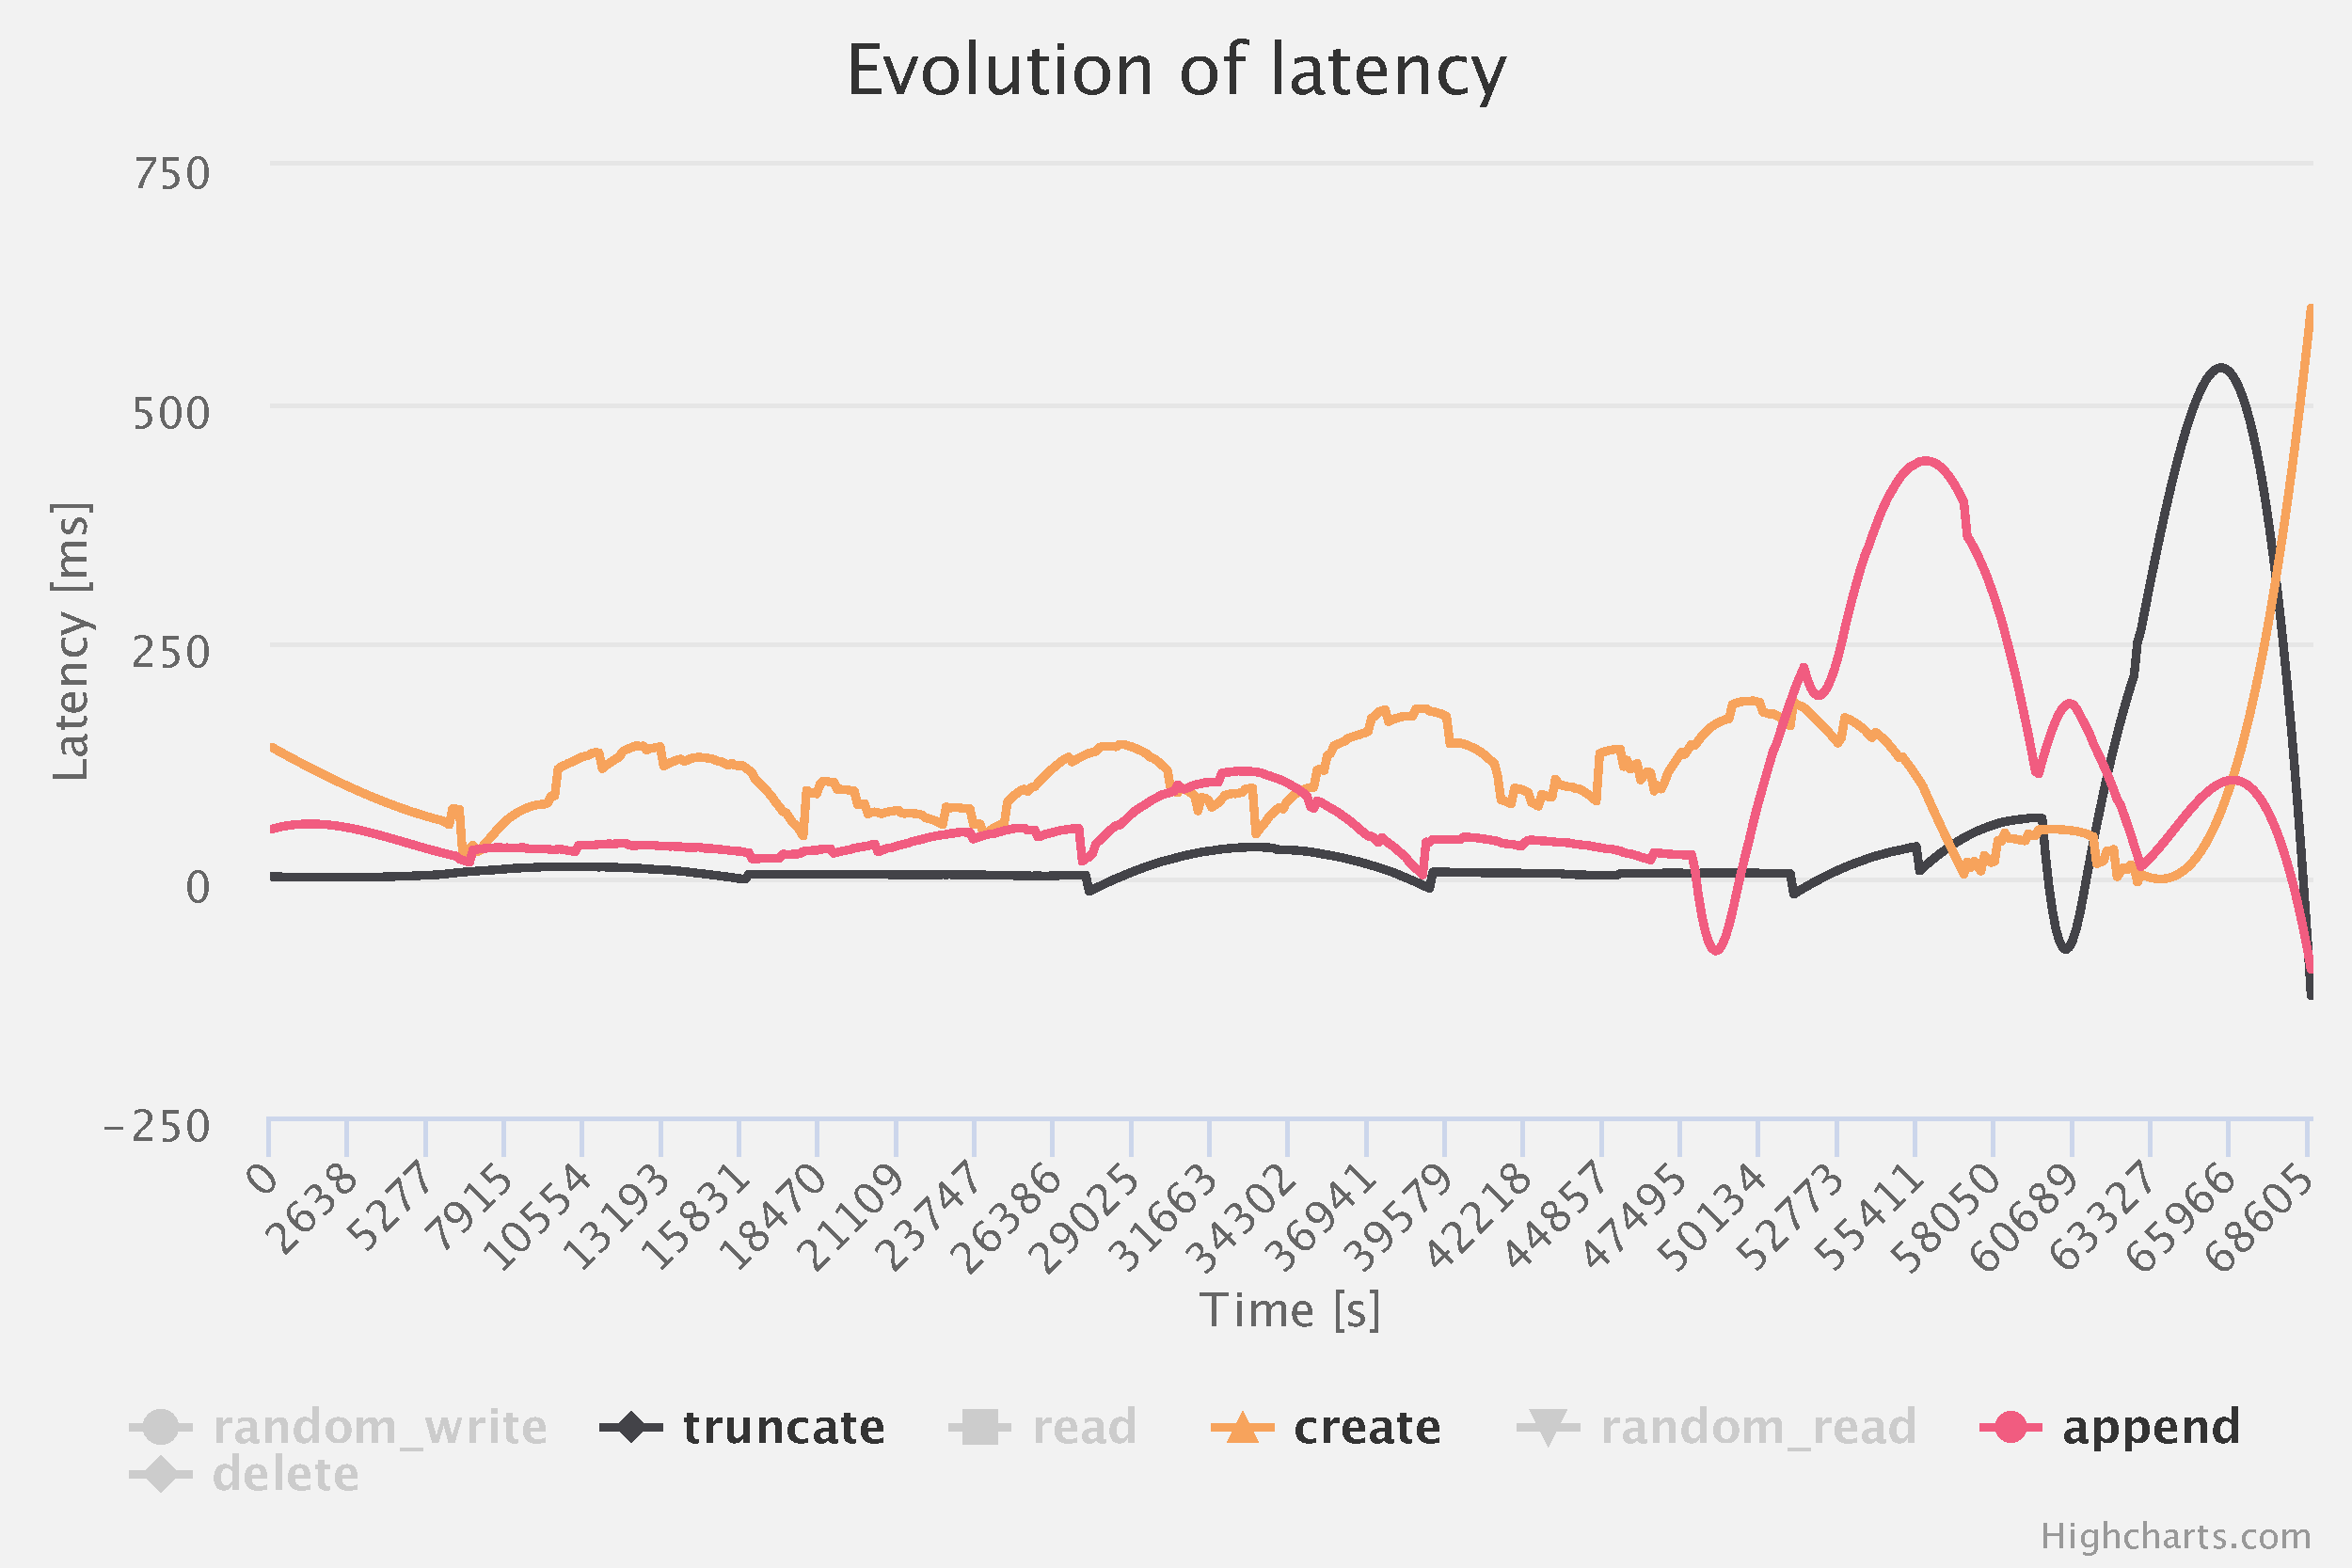
\includegraphics[width=\textwidth]{../charts/HDD_ext4/cta}
        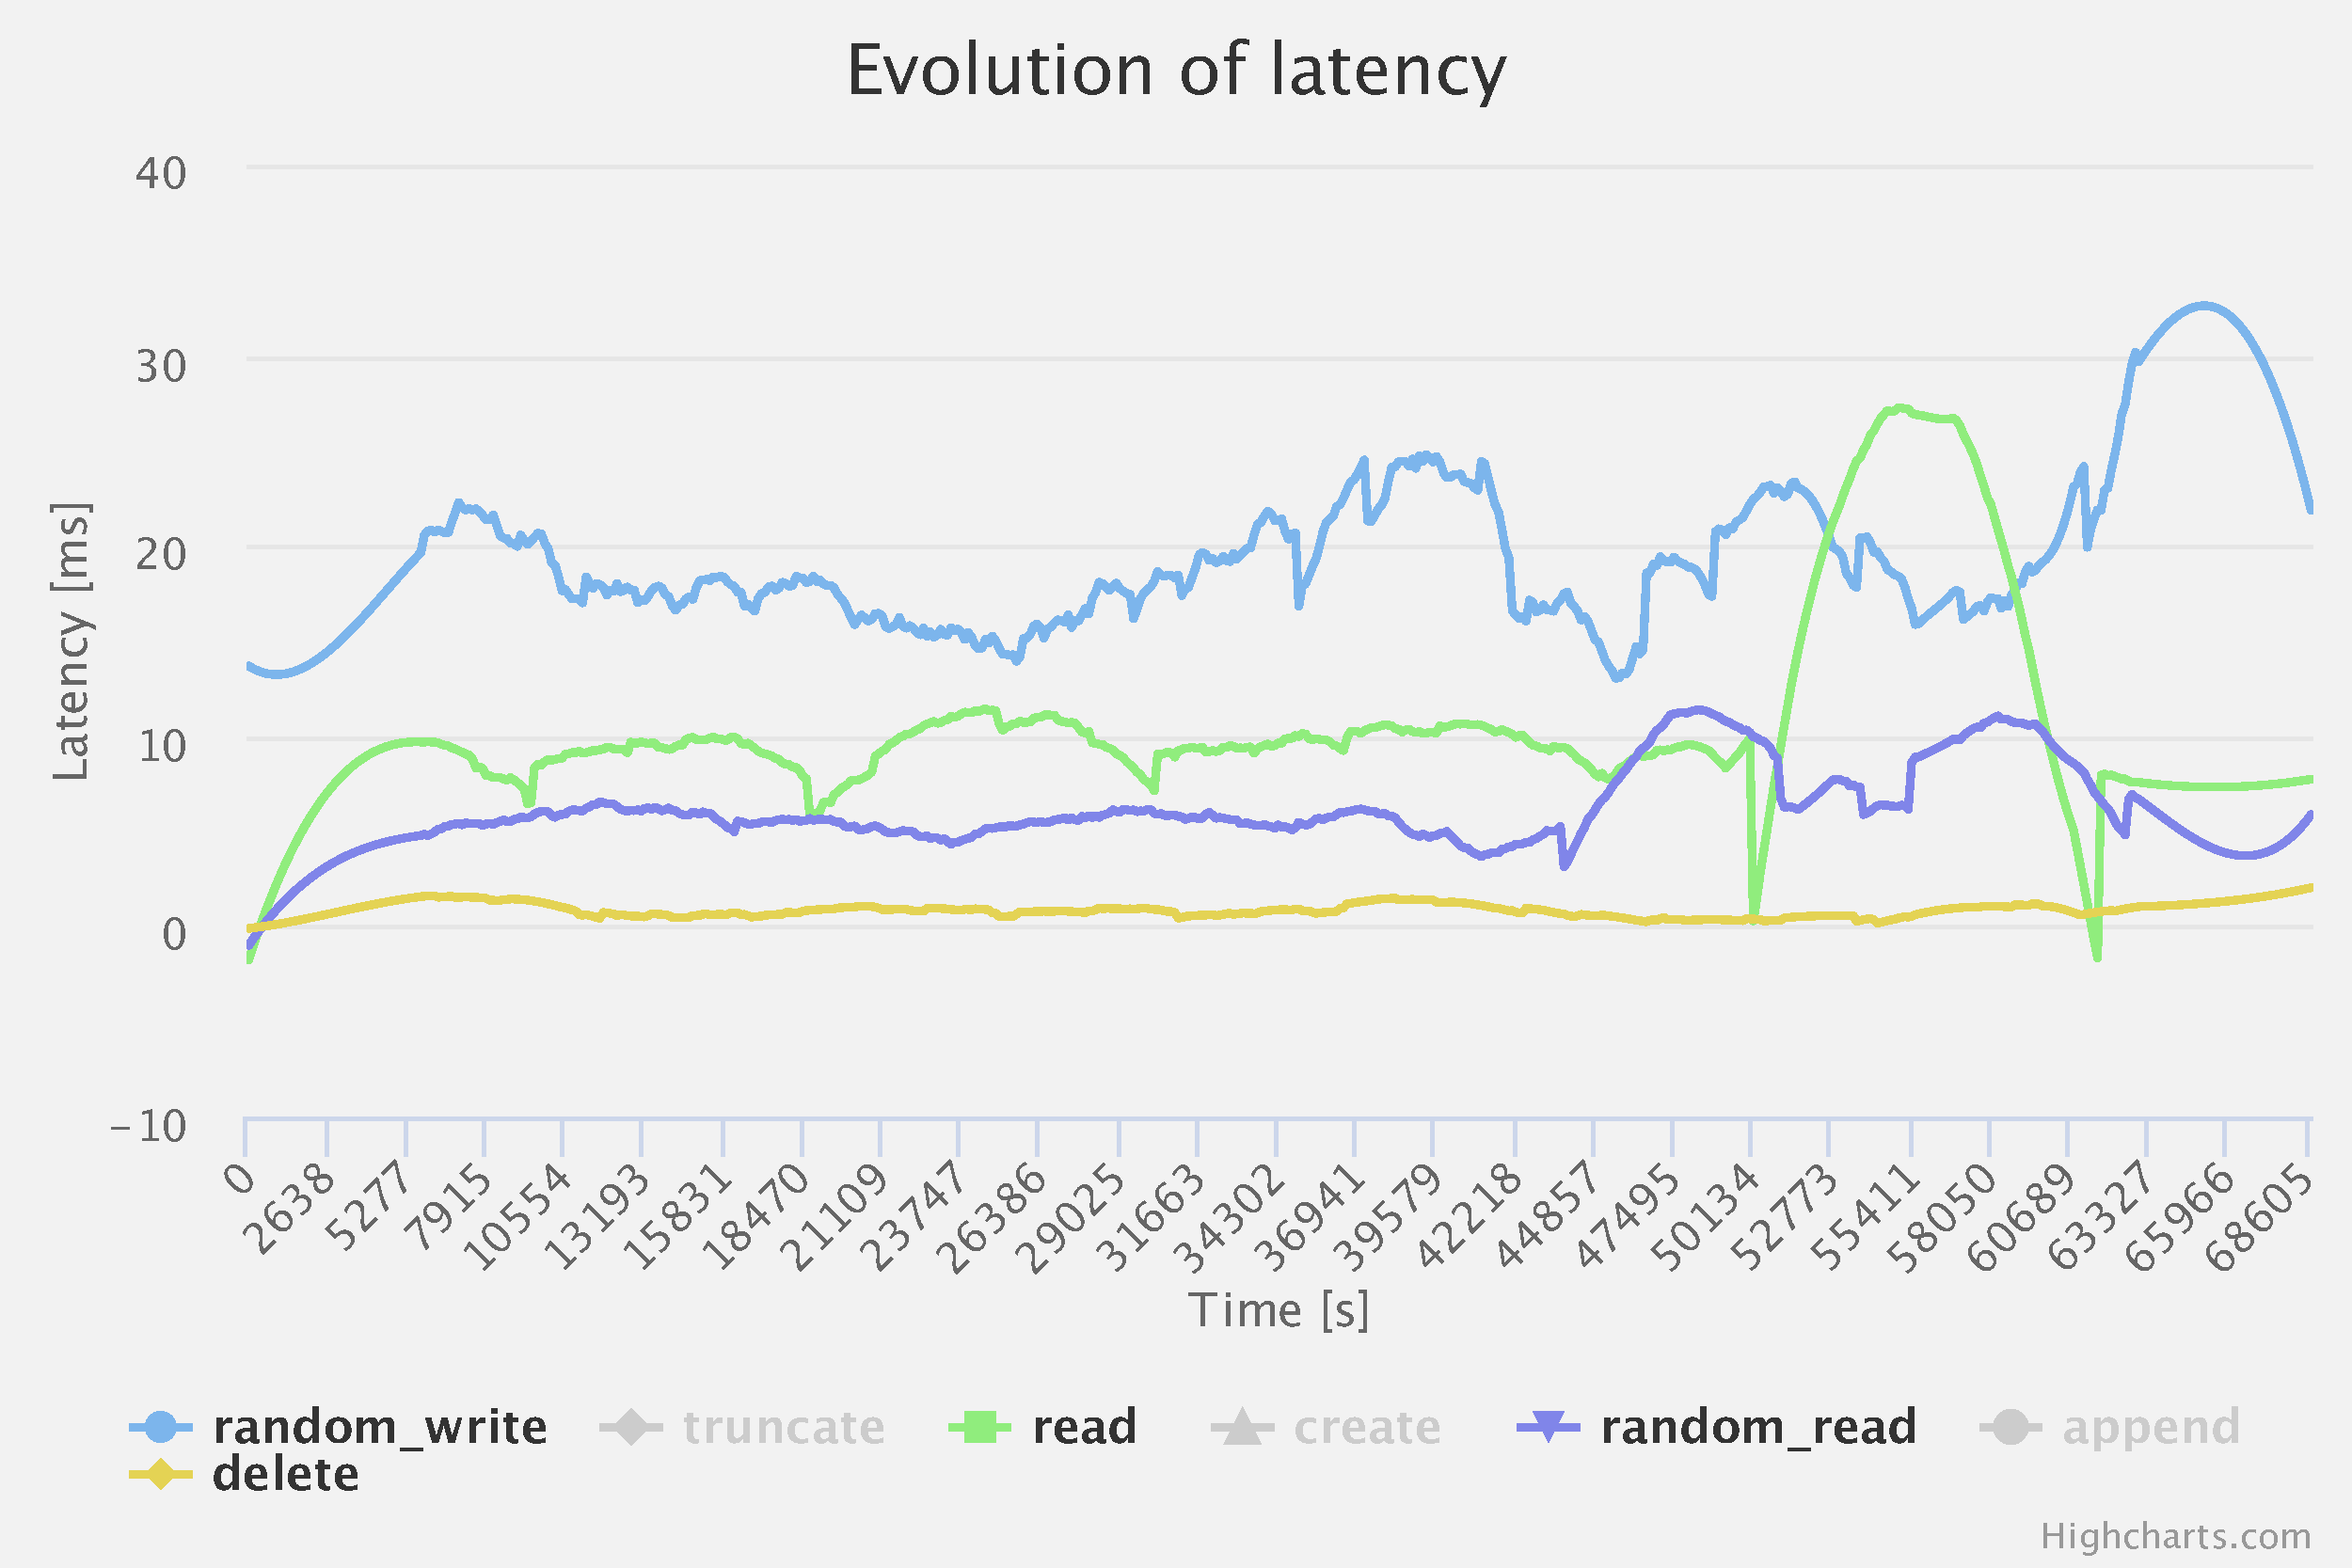
\includegraphics[width=\textwidth]{../charts/HDD_ext4/rrrd}
                \caption[Evolution of latencies of ext4 during testing of high utilisation of HDD]{Evolution of latencies of conducted IO operations during testing of ext4 with high utilisation. Progressively larger fluctuations can be seen in operations truncate and append.}
\label{fig:lats_ext4}
    \end{minipage}
\end{figure}

\clearpage



\section{Test of XFS on SSD with regular trimming}
\begin{itemize}
\itemsep0em 
   \item System: Machine\,2
   \item OS: RHEL-7.3
   \item Kernel: 3.10.0-514.el7.x86\_64
\end{itemize}

\begin{figure}[h]
    \centering
    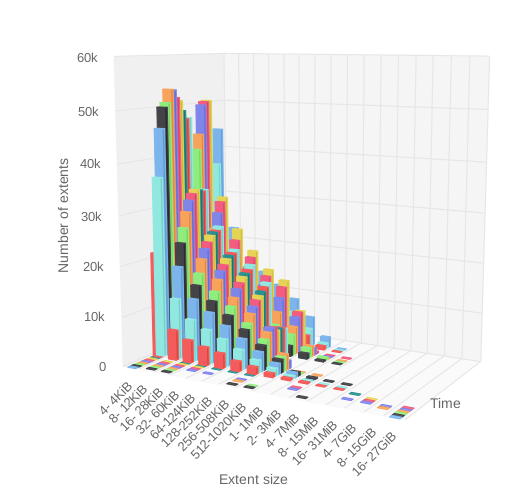
\includegraphics[width=\textwidth,keepaspectratio]{../charts/SSD_xfs_trim/free.png}
    \caption[Evolution of free space fragmentation of XFS during testing on SSD with regular trimming]{This chart shows evolution of free space fragmentation through the whole test. When comparing this chart with Figure~\ref{fig:usage_xfs_ssd_trim}, we can see large raise of number of extents occurred after the test consumed all the available volume.}
    \label{fig:free_xfs_ssd_trim}
\end{figure}

\begin{figure}[h]
    \centering
    \fbox{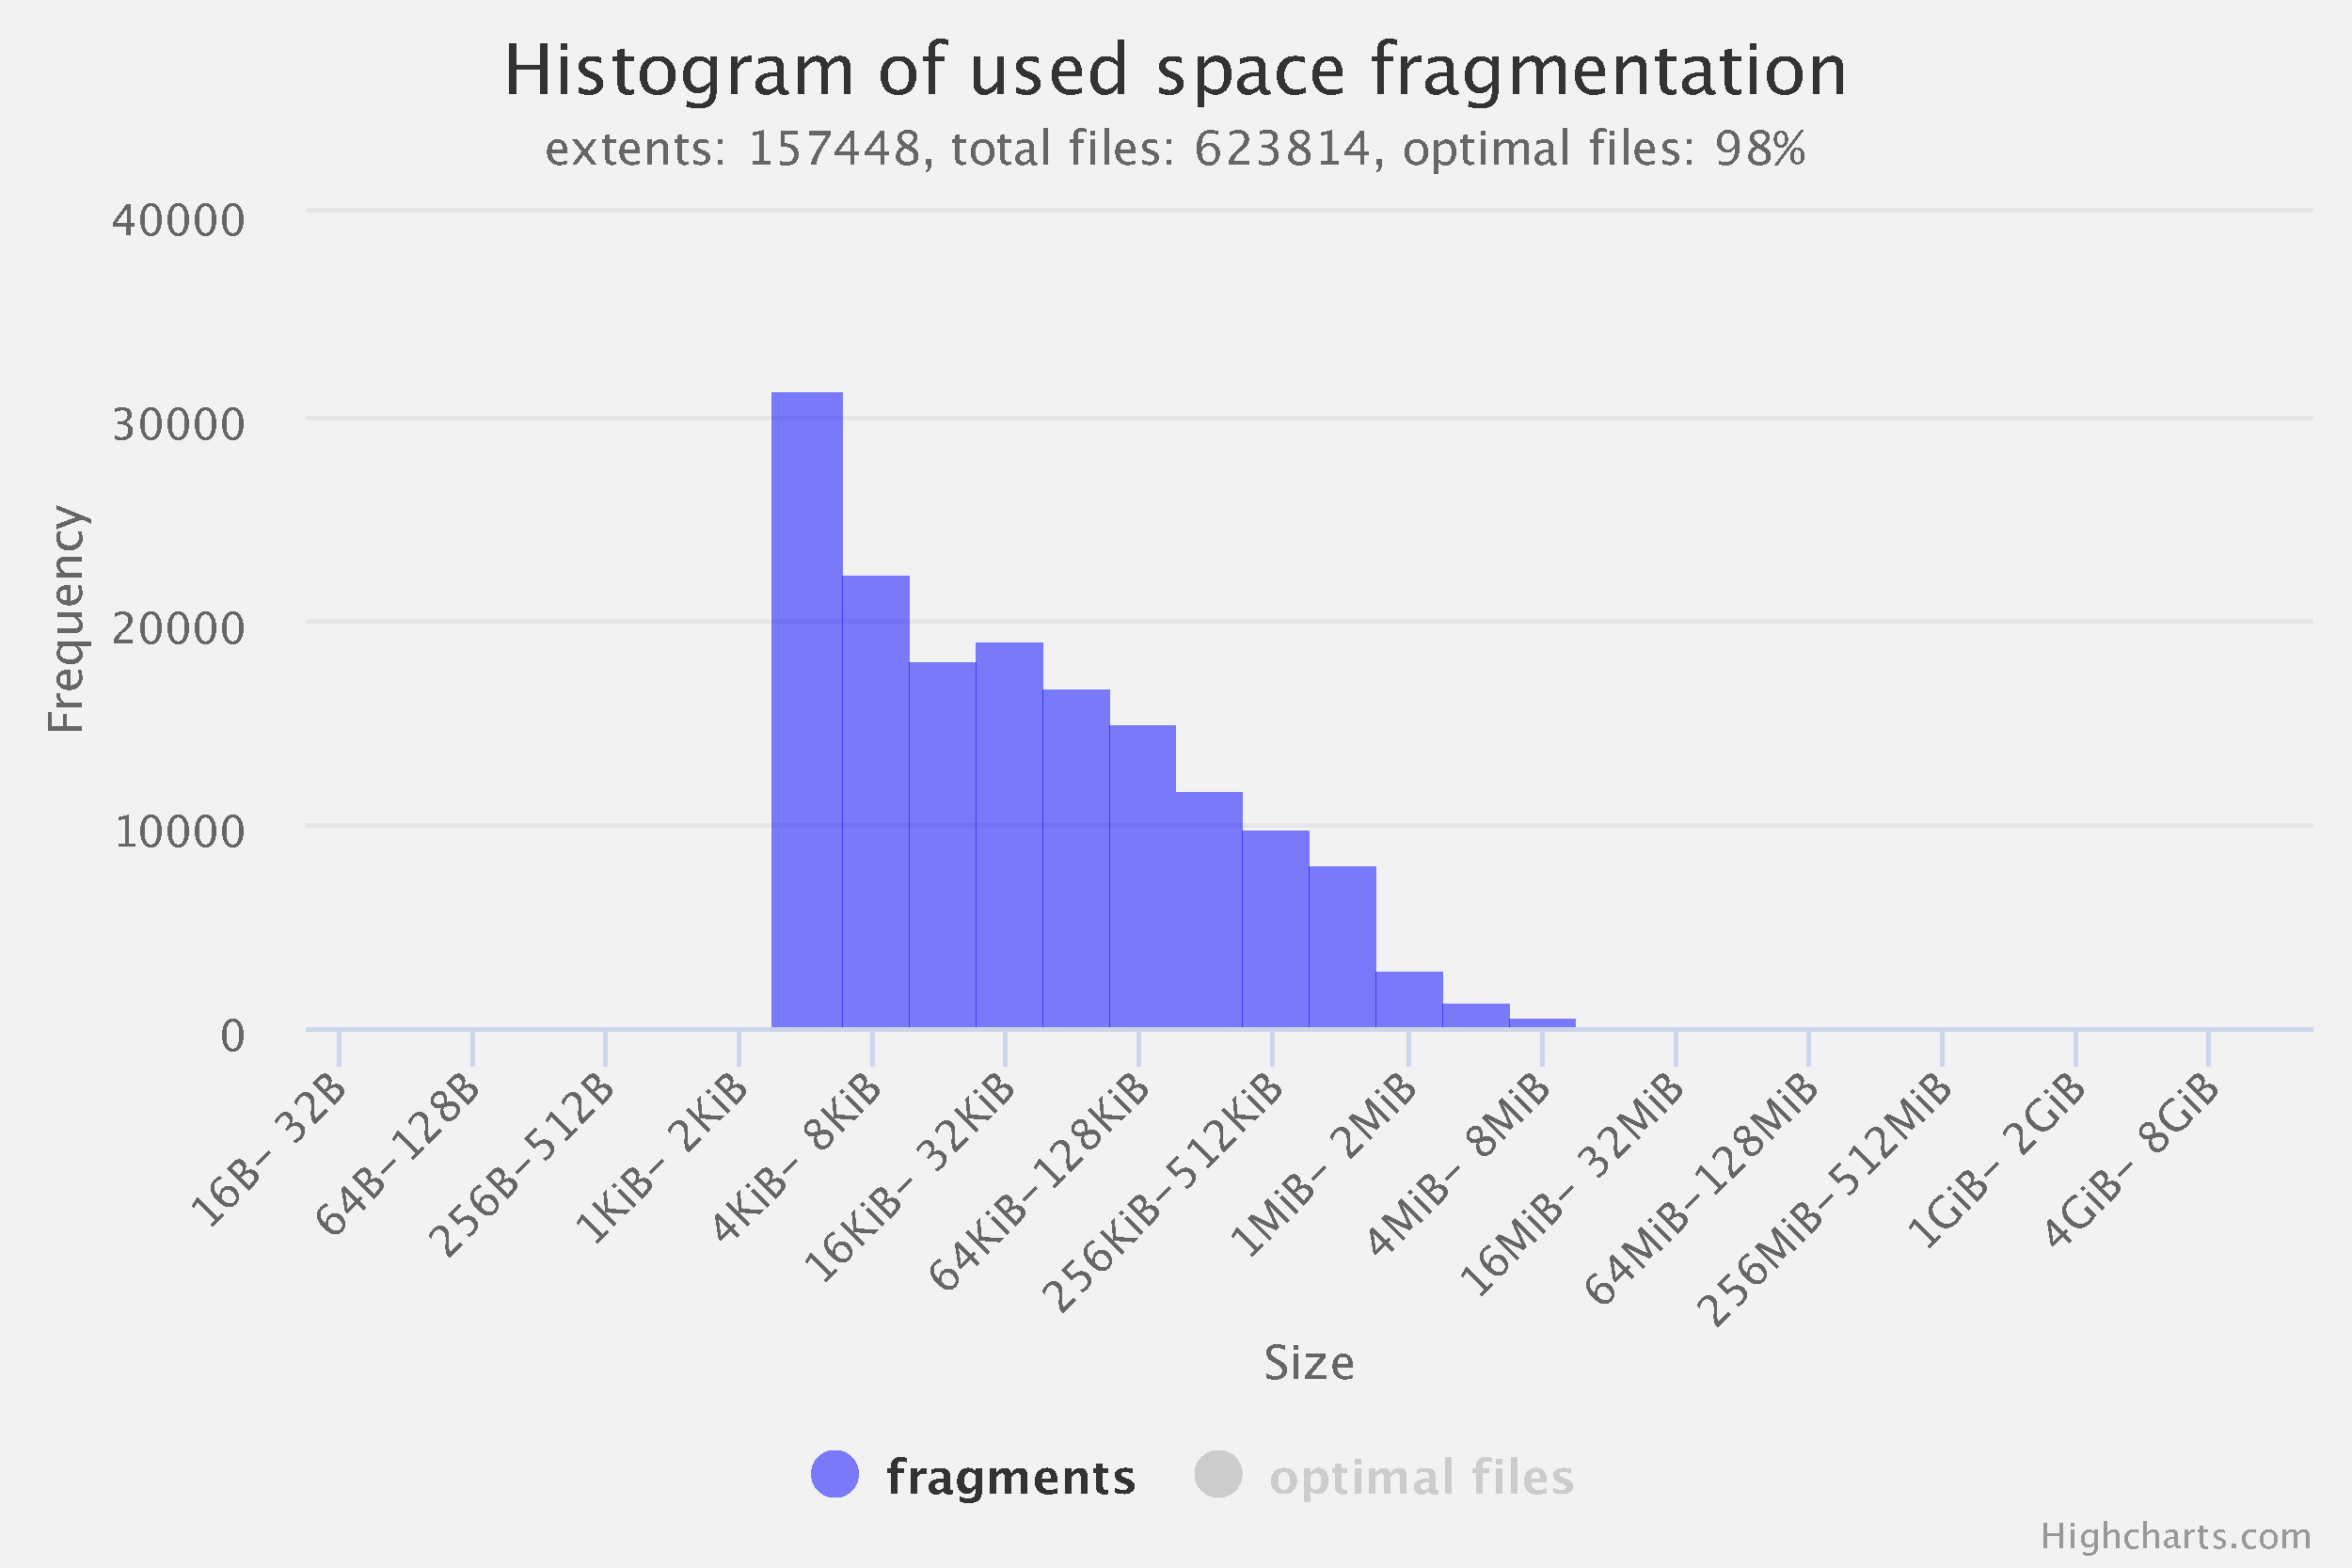
\includegraphics[width=\textwidth,keepaspectratio]{../charts/SSD_xfs_trim/used}}
    \caption[Size distribution of file extents of XFS during testing on SSD with regular trimming]{On this chart, we can see distribution of size of file extents. Despite high fragmentation of free space during the test, the final block layout of file system have around 157 thousands of extents. 98\% of files were optimally allocated. Furthermore, we can observe that extent size distribution is similar to file size distribution in the test. Please note that smallest possible extent size in file system is the size of its block size ($\SI{4}{\kilo\byte}$ by default).}
    \label{fig:used_xfs_ssd_trim}
\end{figure}

\begin{figure}[!h]
    \begin{minipage}{\textwidth}
        \centering
        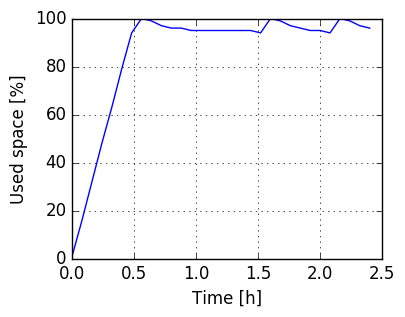
\includegraphics[width=0.7\textwidth]{../charts/SSD_xfs_trim/usage.png}
        \caption[Usage of available space of XFS during testing on SSD with regular trimming]{Chart displays file system utilisation over time. Test filled the available volume ($\SI{120}{\giga\byte}$) in half an hour. It is difficult to say how many volume deleting iterations were triggered, because the test managed to fill released space between usage logging intervals.}
\label{fig:usage_xfs_ssd_trim}
    \end{minipage}
\end{figure}

\begin{figure}[!htb]
    \centering
   \begin{minipage}{\textwidth}
        \centering
        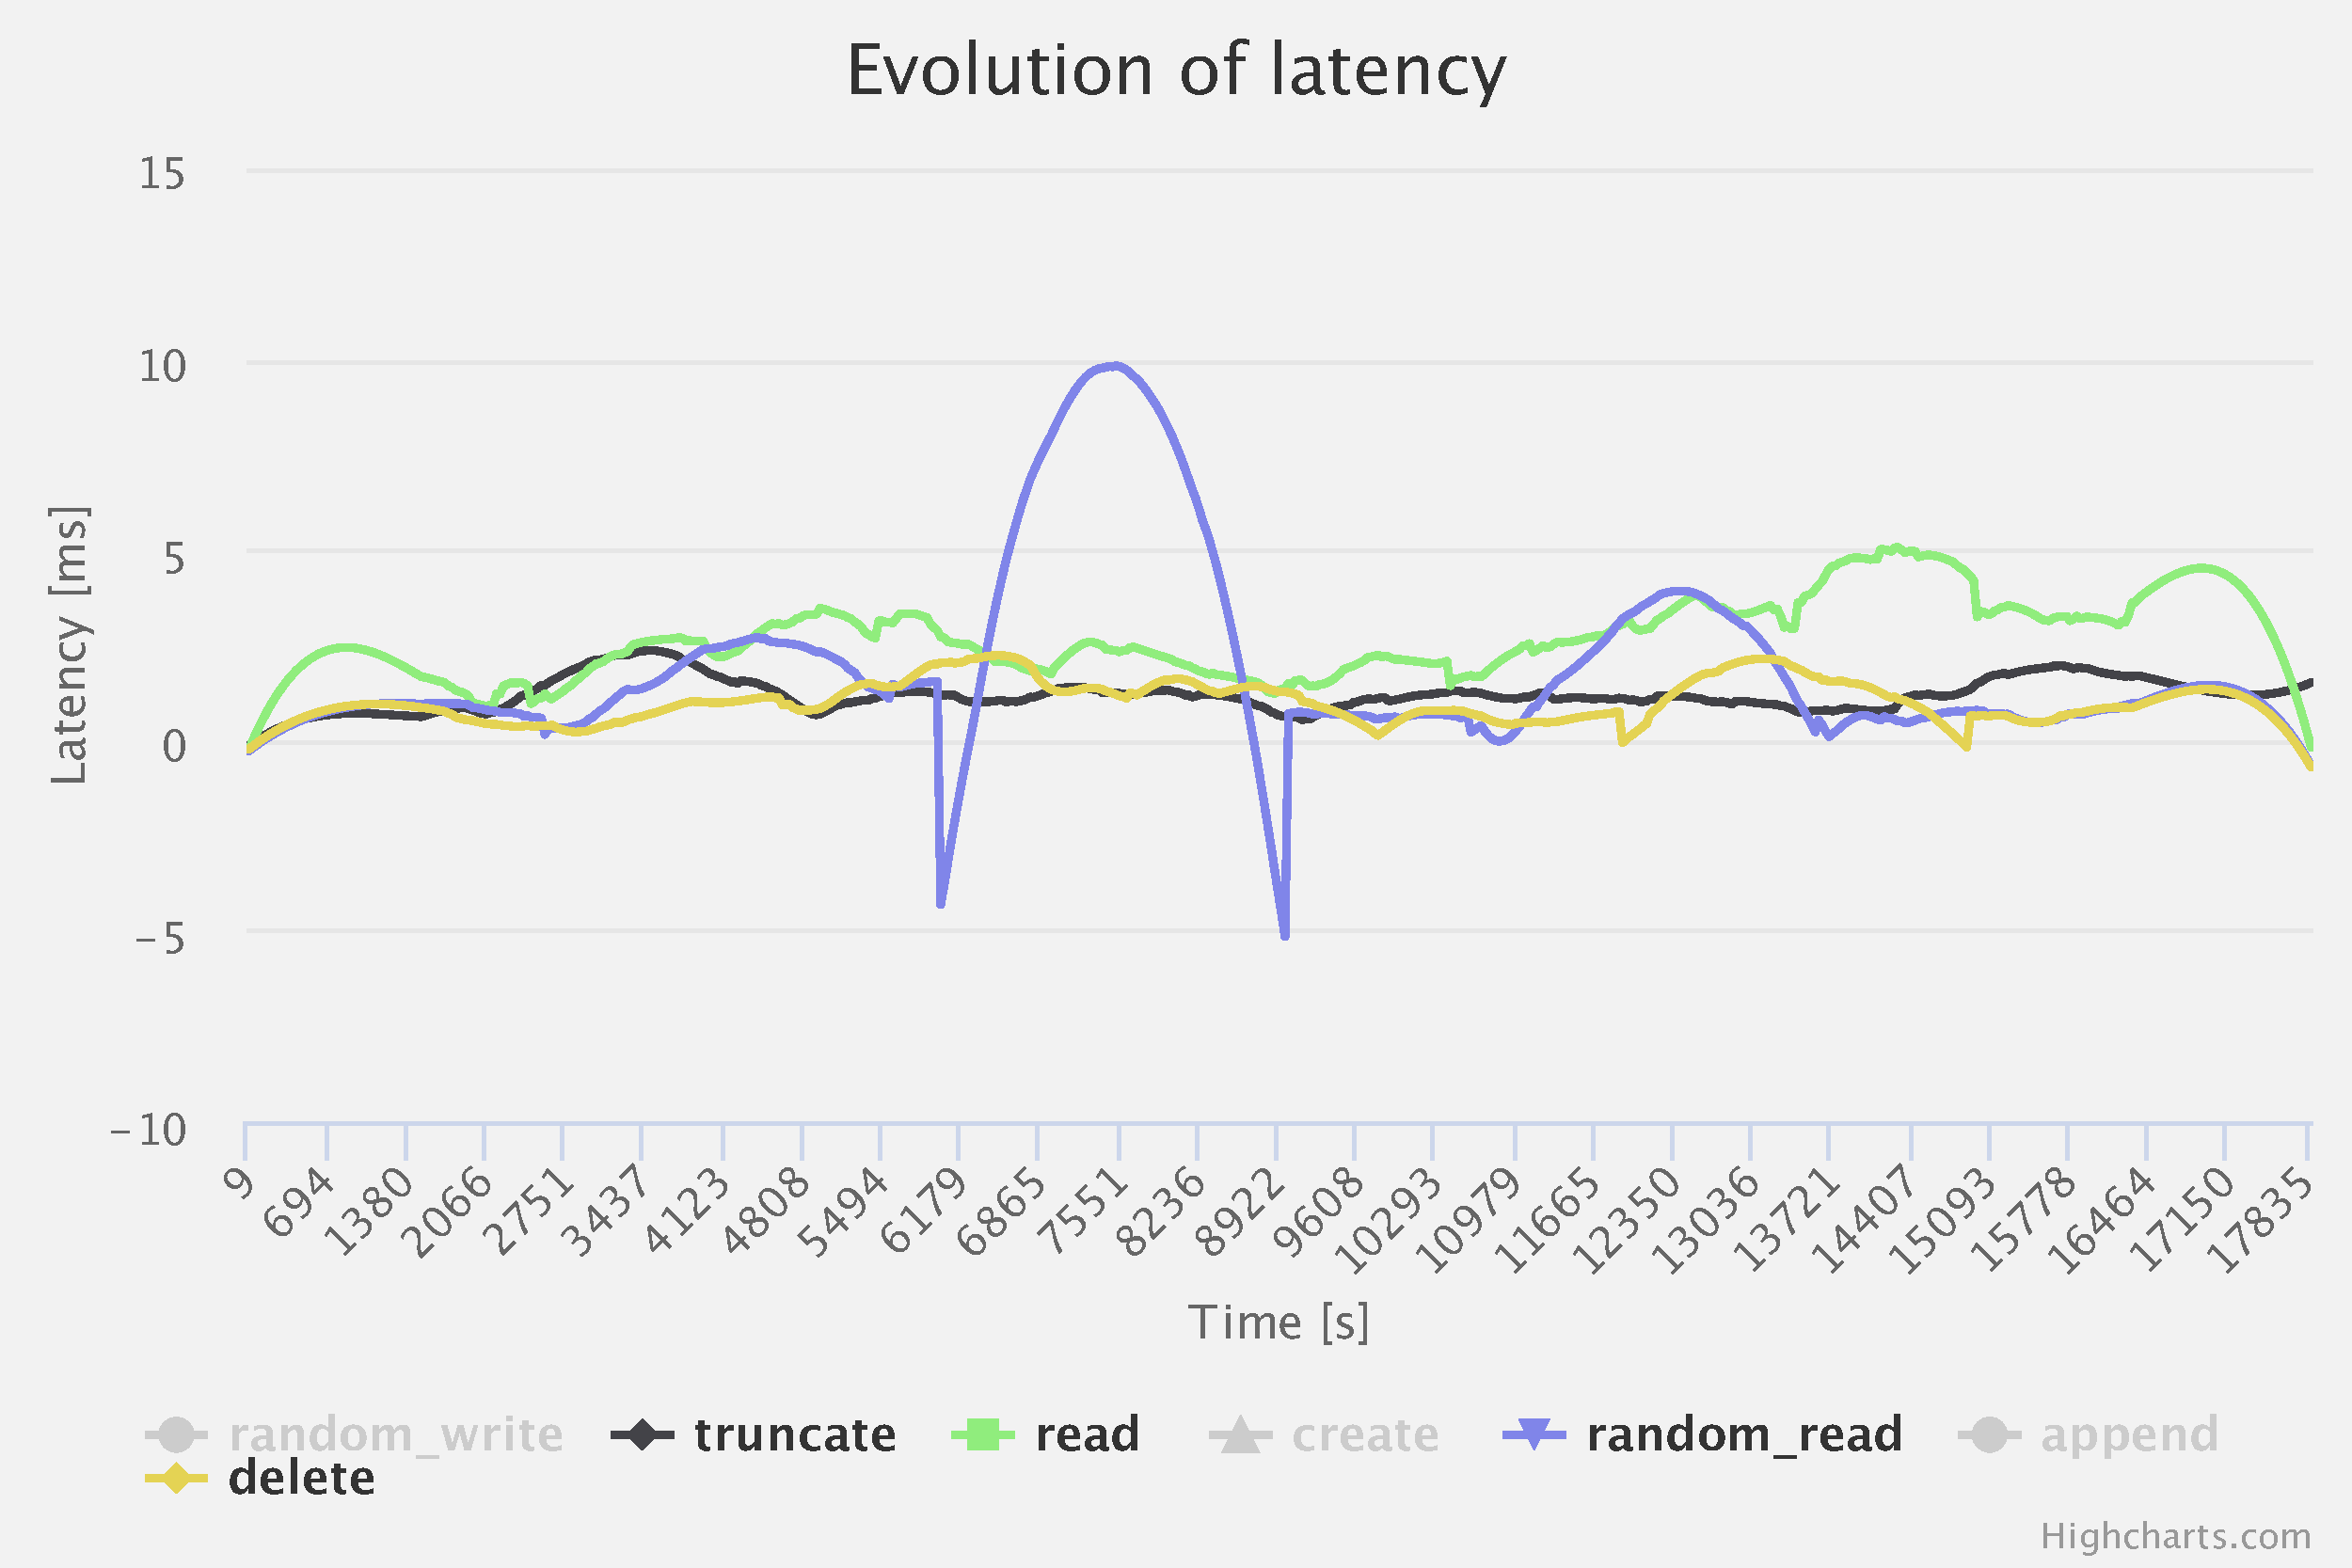
\includegraphics[width=\textwidth]{../charts/SSD_xfs_trim/1}
        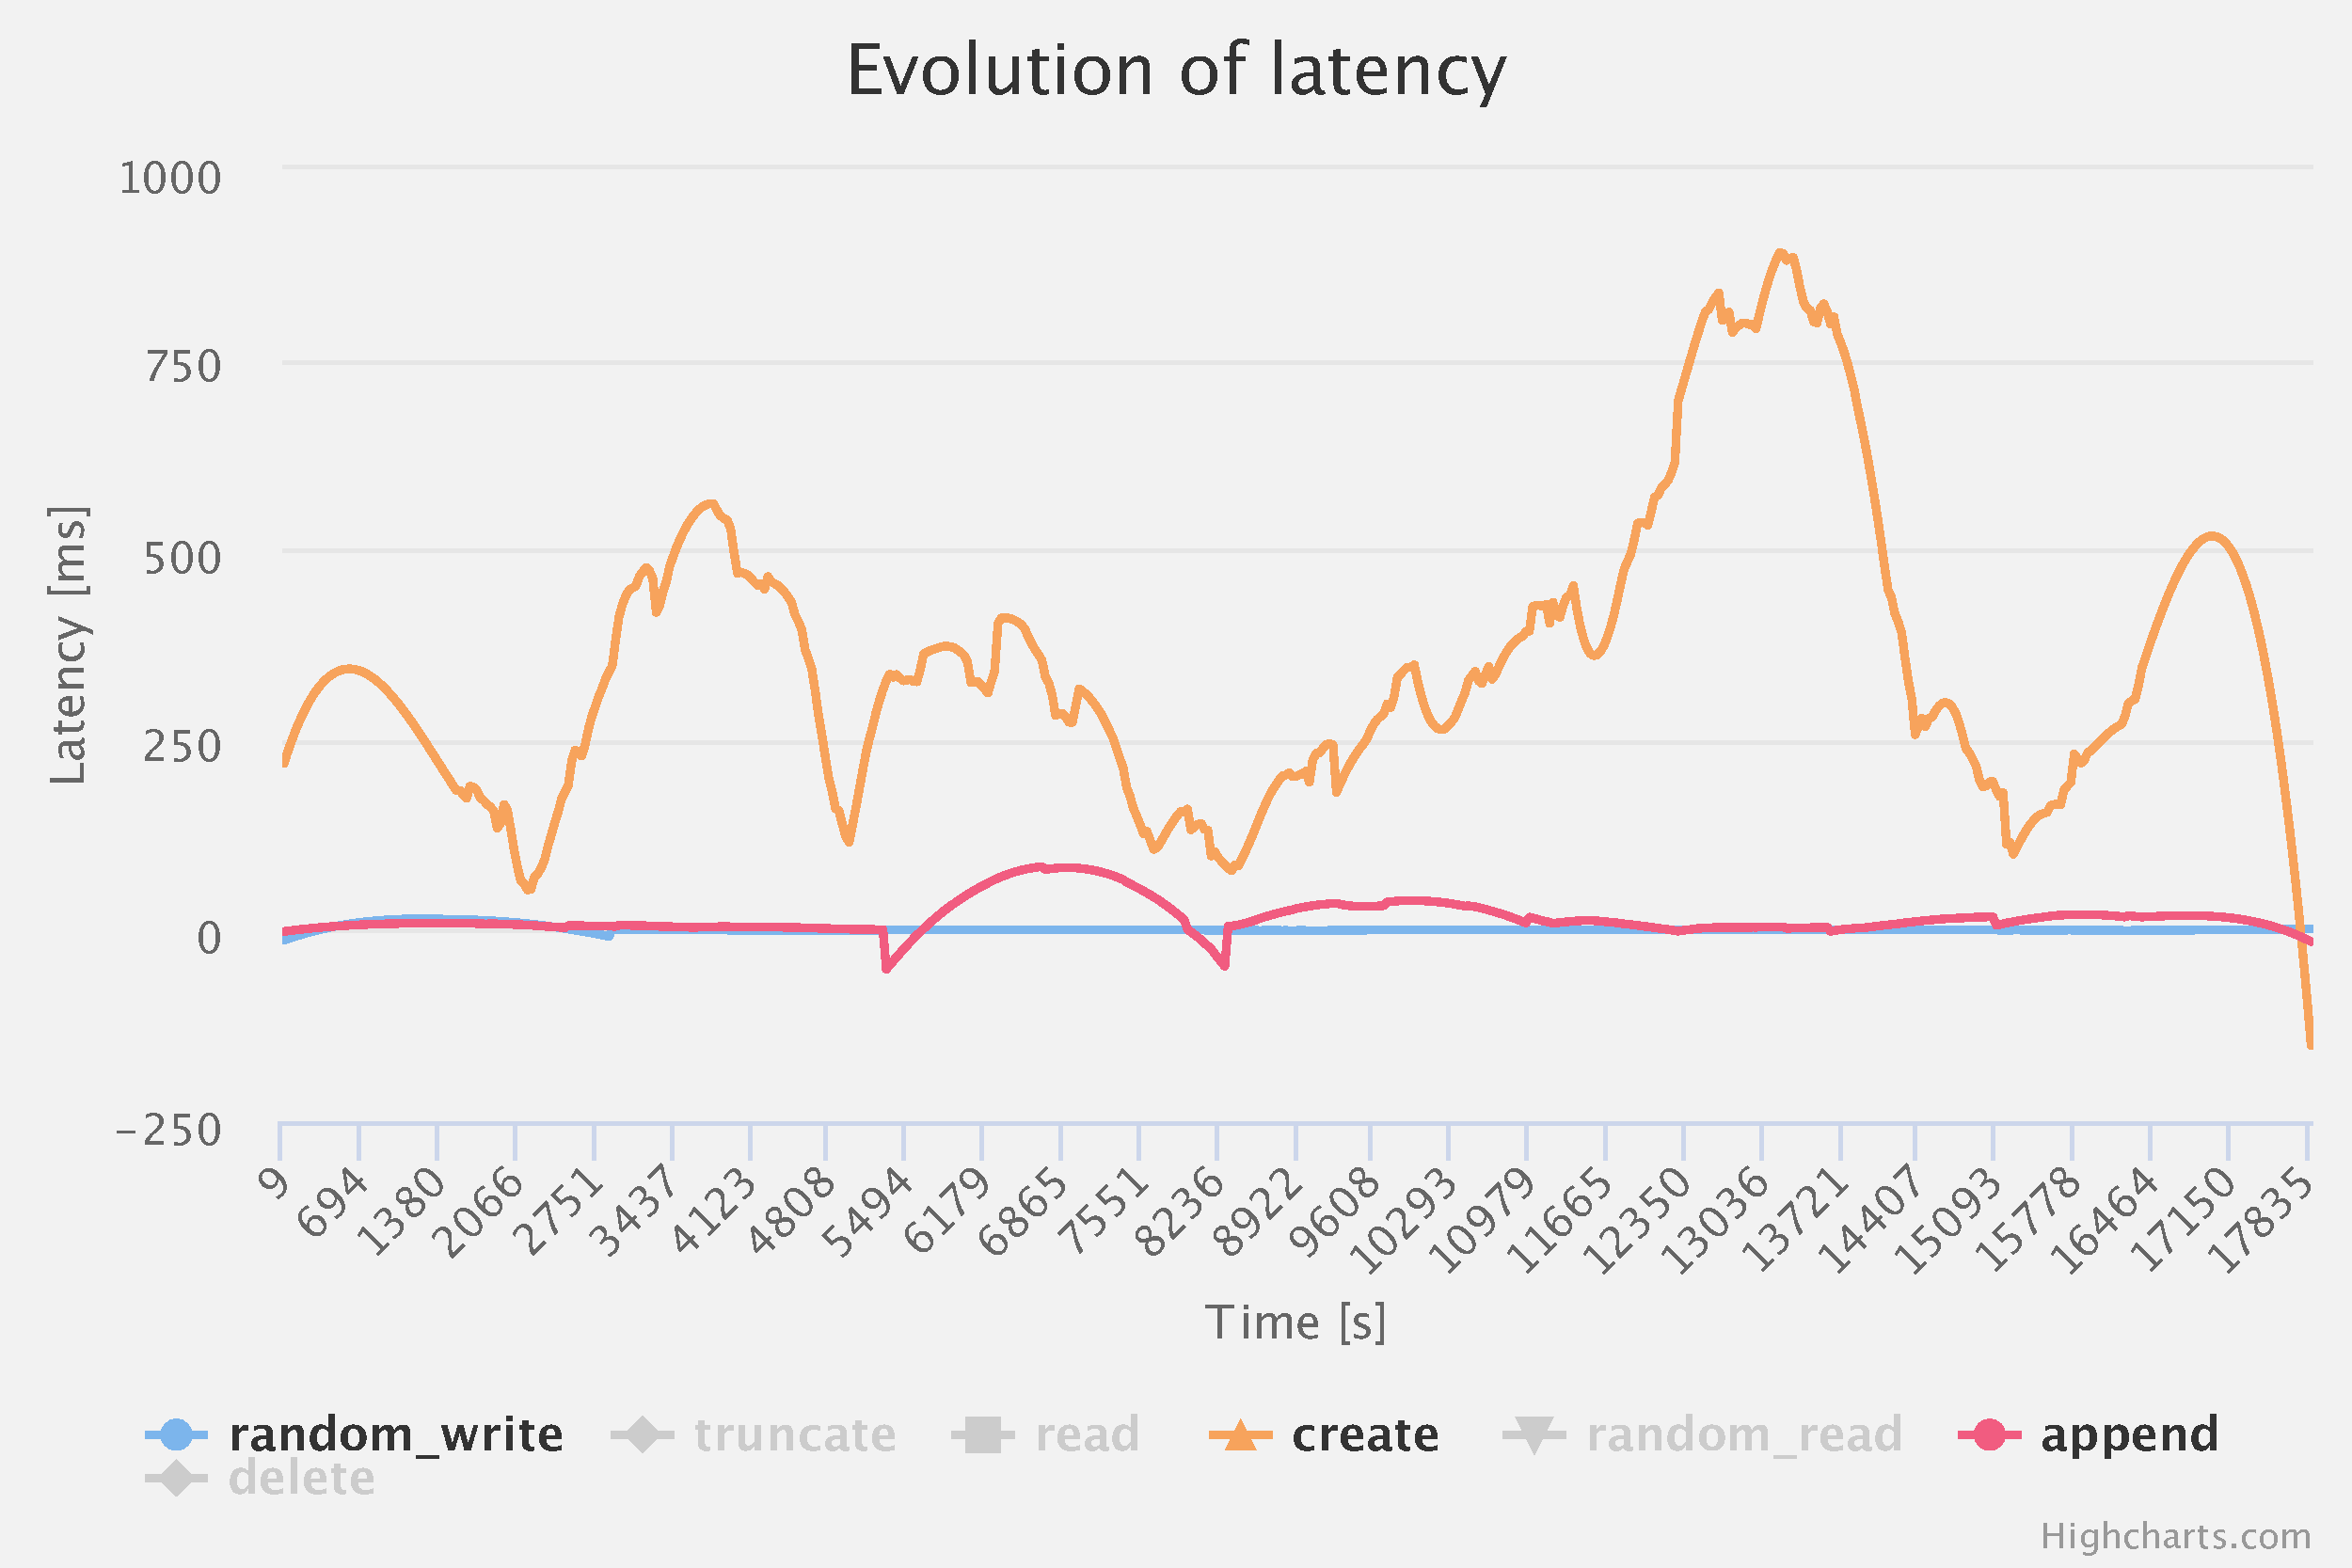
\includegraphics[width=\textwidth]{../charts/SSD_xfs_trim/2}
                \caption[Evolution of latencies of XFS during testing on SSD with regular trimming]{Evolution of latencies of conducted IO operations during testing XFS on SSD device with regular trimming performed.}
\label{fig:lats_xfs_ssd_trim}

    \end{minipage}
\end{figure}

\clearpage

\section{Test of ext4 on SSD with regular trimming}
\begin{itemize}
\itemsep0em 
   \item System: Machine\,2
   \item OS: RHEL-7.3
   \item Kernel: 3.10.0-514.el7.x86\_64
\end{itemize}

\begin{figure}[h]
    \centering
    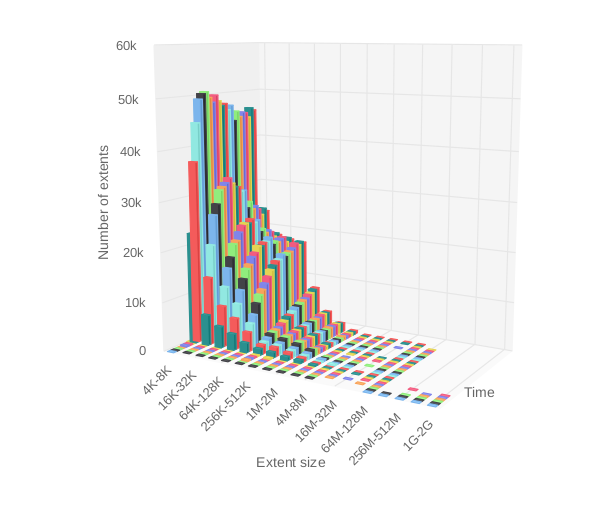
\includegraphics[width=\textwidth,keepaspectratio]{../charts/SSD_ext4_trim/free.png}
    \caption[Evolution of free space fragmentation of ext4 during testing on SSD with regular trimming]{This chart shows evolution of free space fragmentation through the whole test. When comparing this chart with Figure~\ref{fig:usage_ext4_ssd_trim}, we can see large raise of number of extents occurred after the test consumed all the available volume.}
    \label{fig:free_ext4_ssd}
\end{figure}

\begin{figure}[h]
    \centering
    \fbox{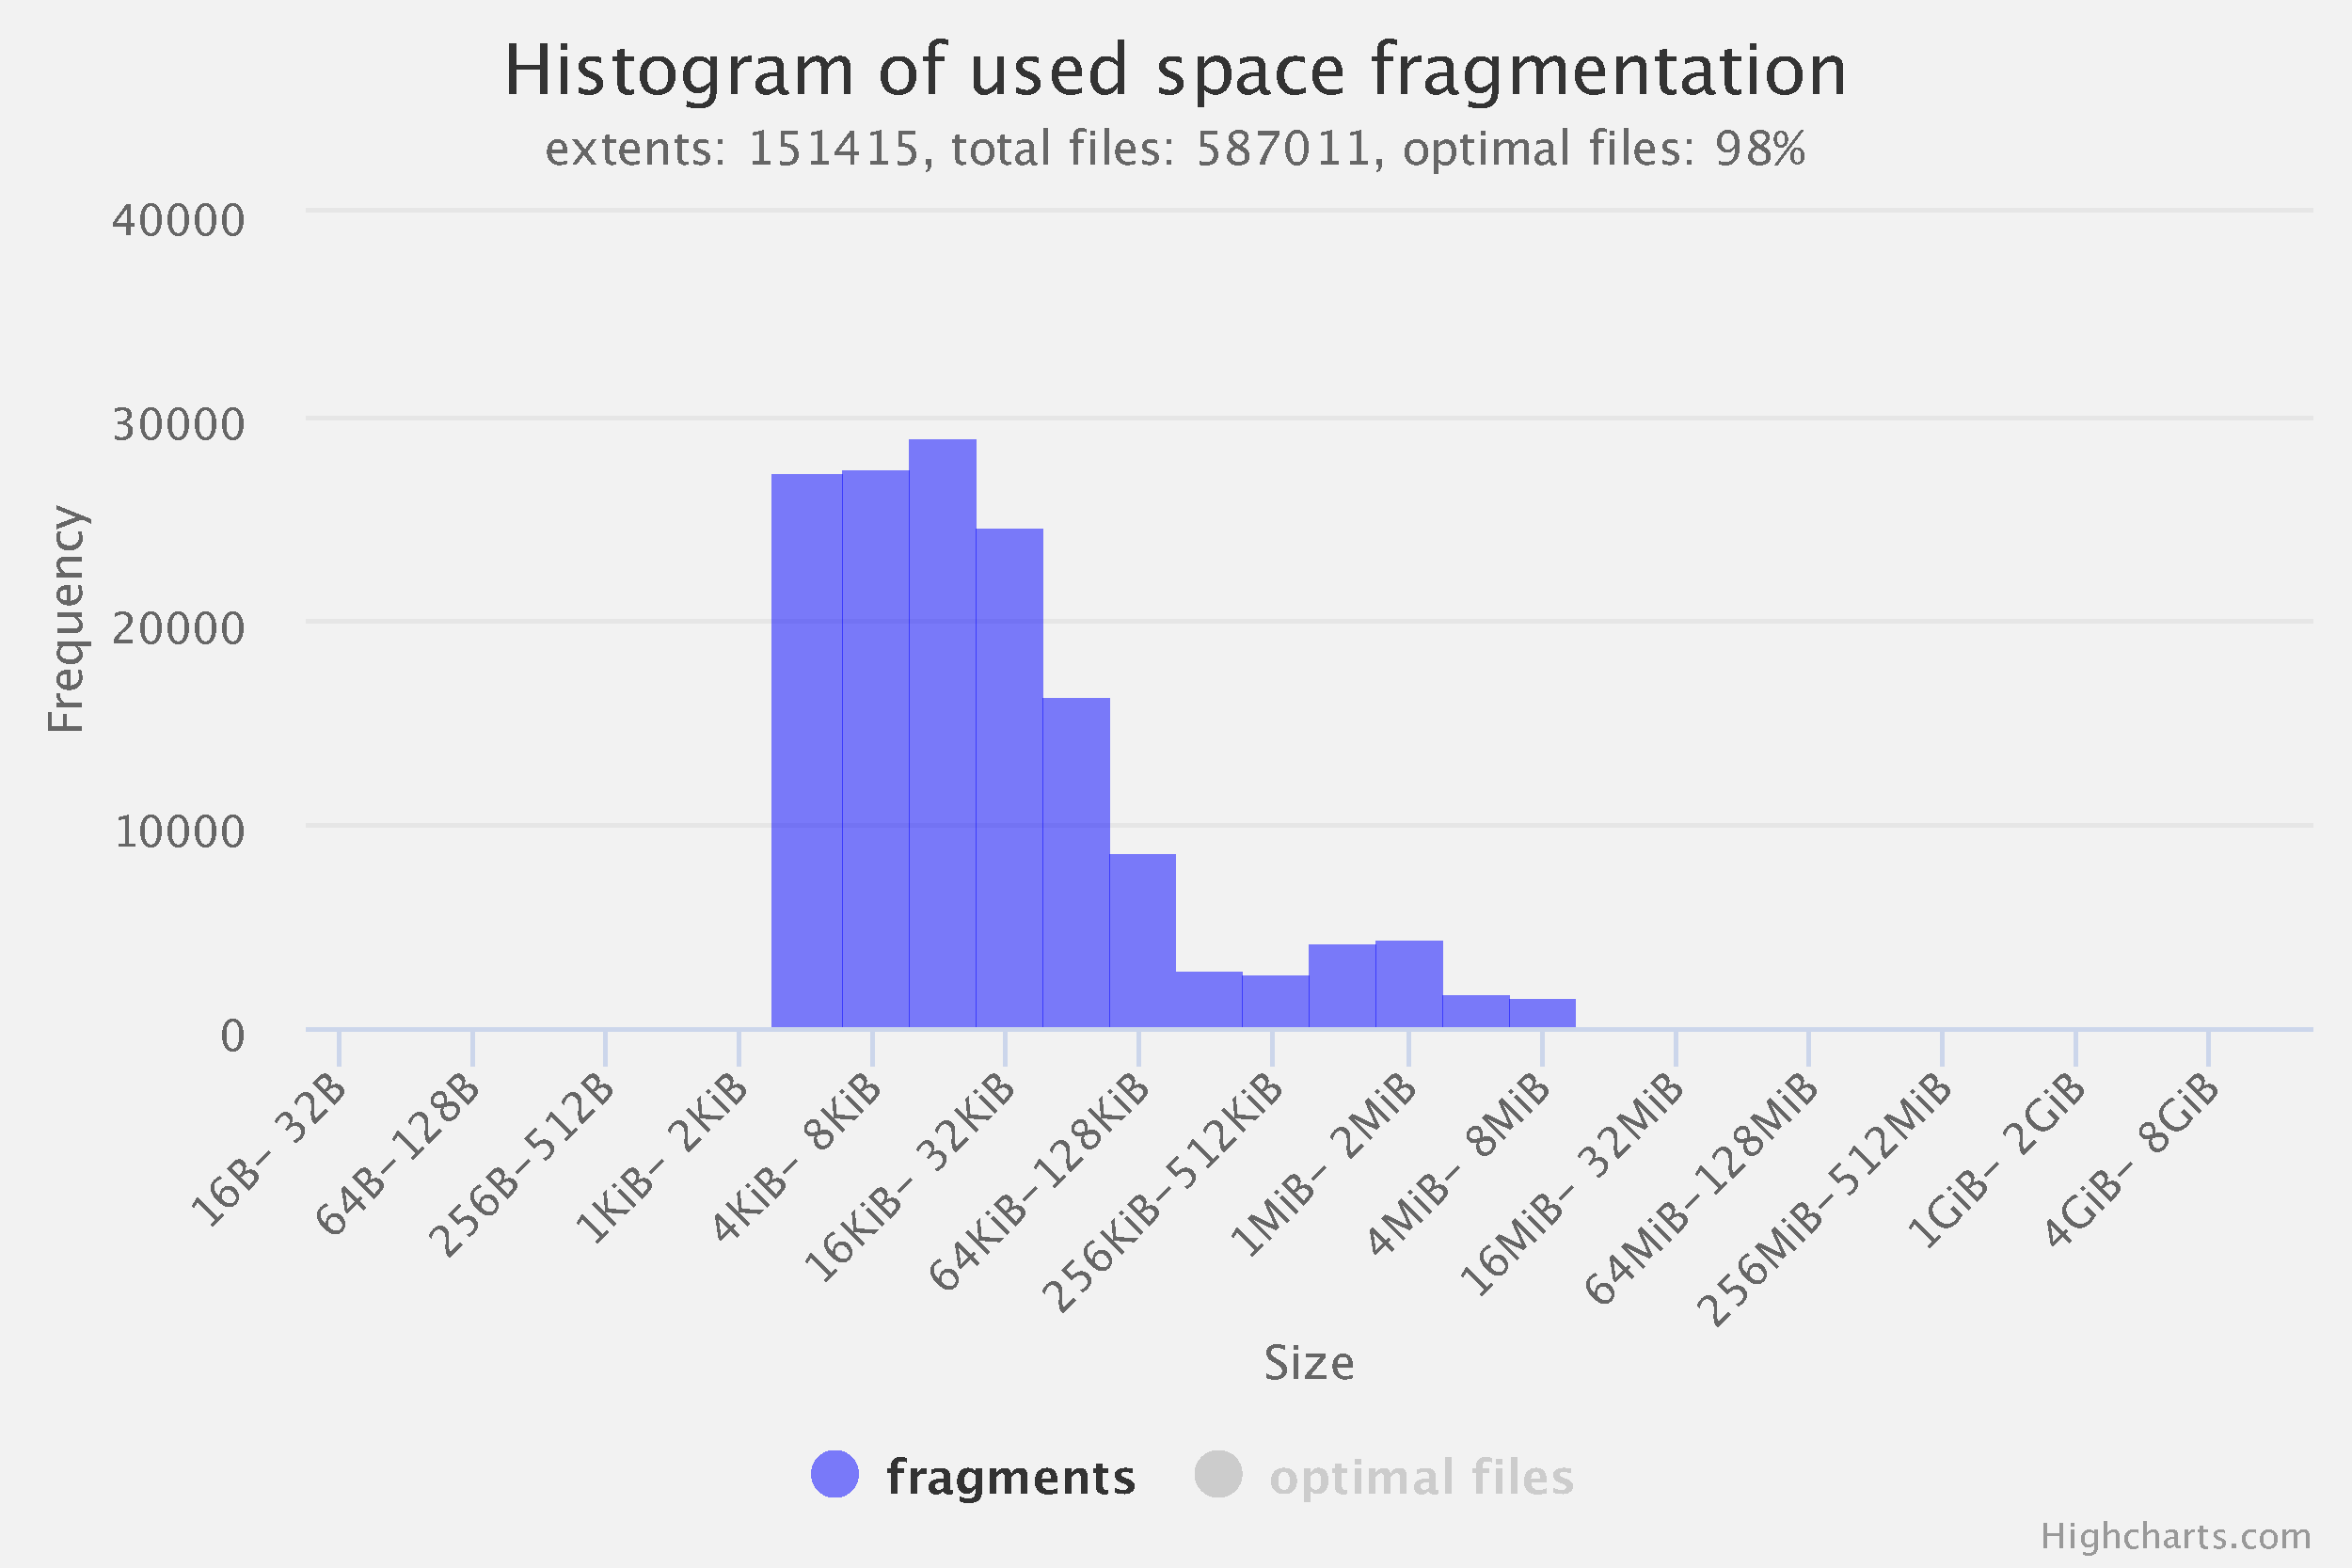
\includegraphics[width=\textwidth,keepaspectratio]{../charts/SSD_ext4_trim/used}}
    \caption[Size distribution of file extents of ext4 during testing on SSD with regular trimming]{On this chart, we can see distribution of size of file extents. Despite high fragmentation of free space during the test, the final block layout of file system have around 151 thousands of extents. 98\% of files were optimally allocated. Furthermore, we can observe that extent size distribution has lower amount of larger extents (>$\SI{128}{\kilo\byte}$) while having similar amounts of smaller extents (4-$\SI{32}{\kilo\byte}$).}
    \label{fig:used_ext4_ssd}
\end{figure}

\begin{figure}[h]
    \begin{minipage}{\textwidth}
        \centering
        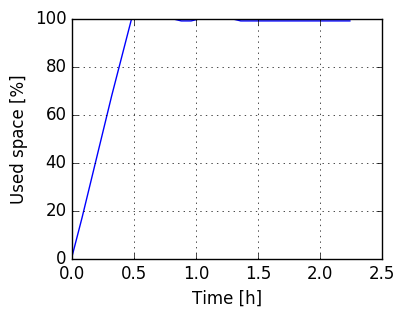
\includegraphics[width=0.7\textwidth]{../charts/SSD_ext4_trim/usage.png}
        \caption[Usage of available space of ext4 during testing on SSD with regular trimming]{Chart displays file system utilisation over time. Test filled the available volume ($\SI{120}{\giga\byte}$) in half an hour. It is difficult to say how many volume deleting iterations were triggered, because the test managed to fill released space between usage logging intervals.}
\label{fig:usage_ext4_ssd_trim}
    \end{minipage}
\end{figure}

\begin{figure}[!htb]
    \centering
   \begin{minipage}{\textwidth}
        \centering
        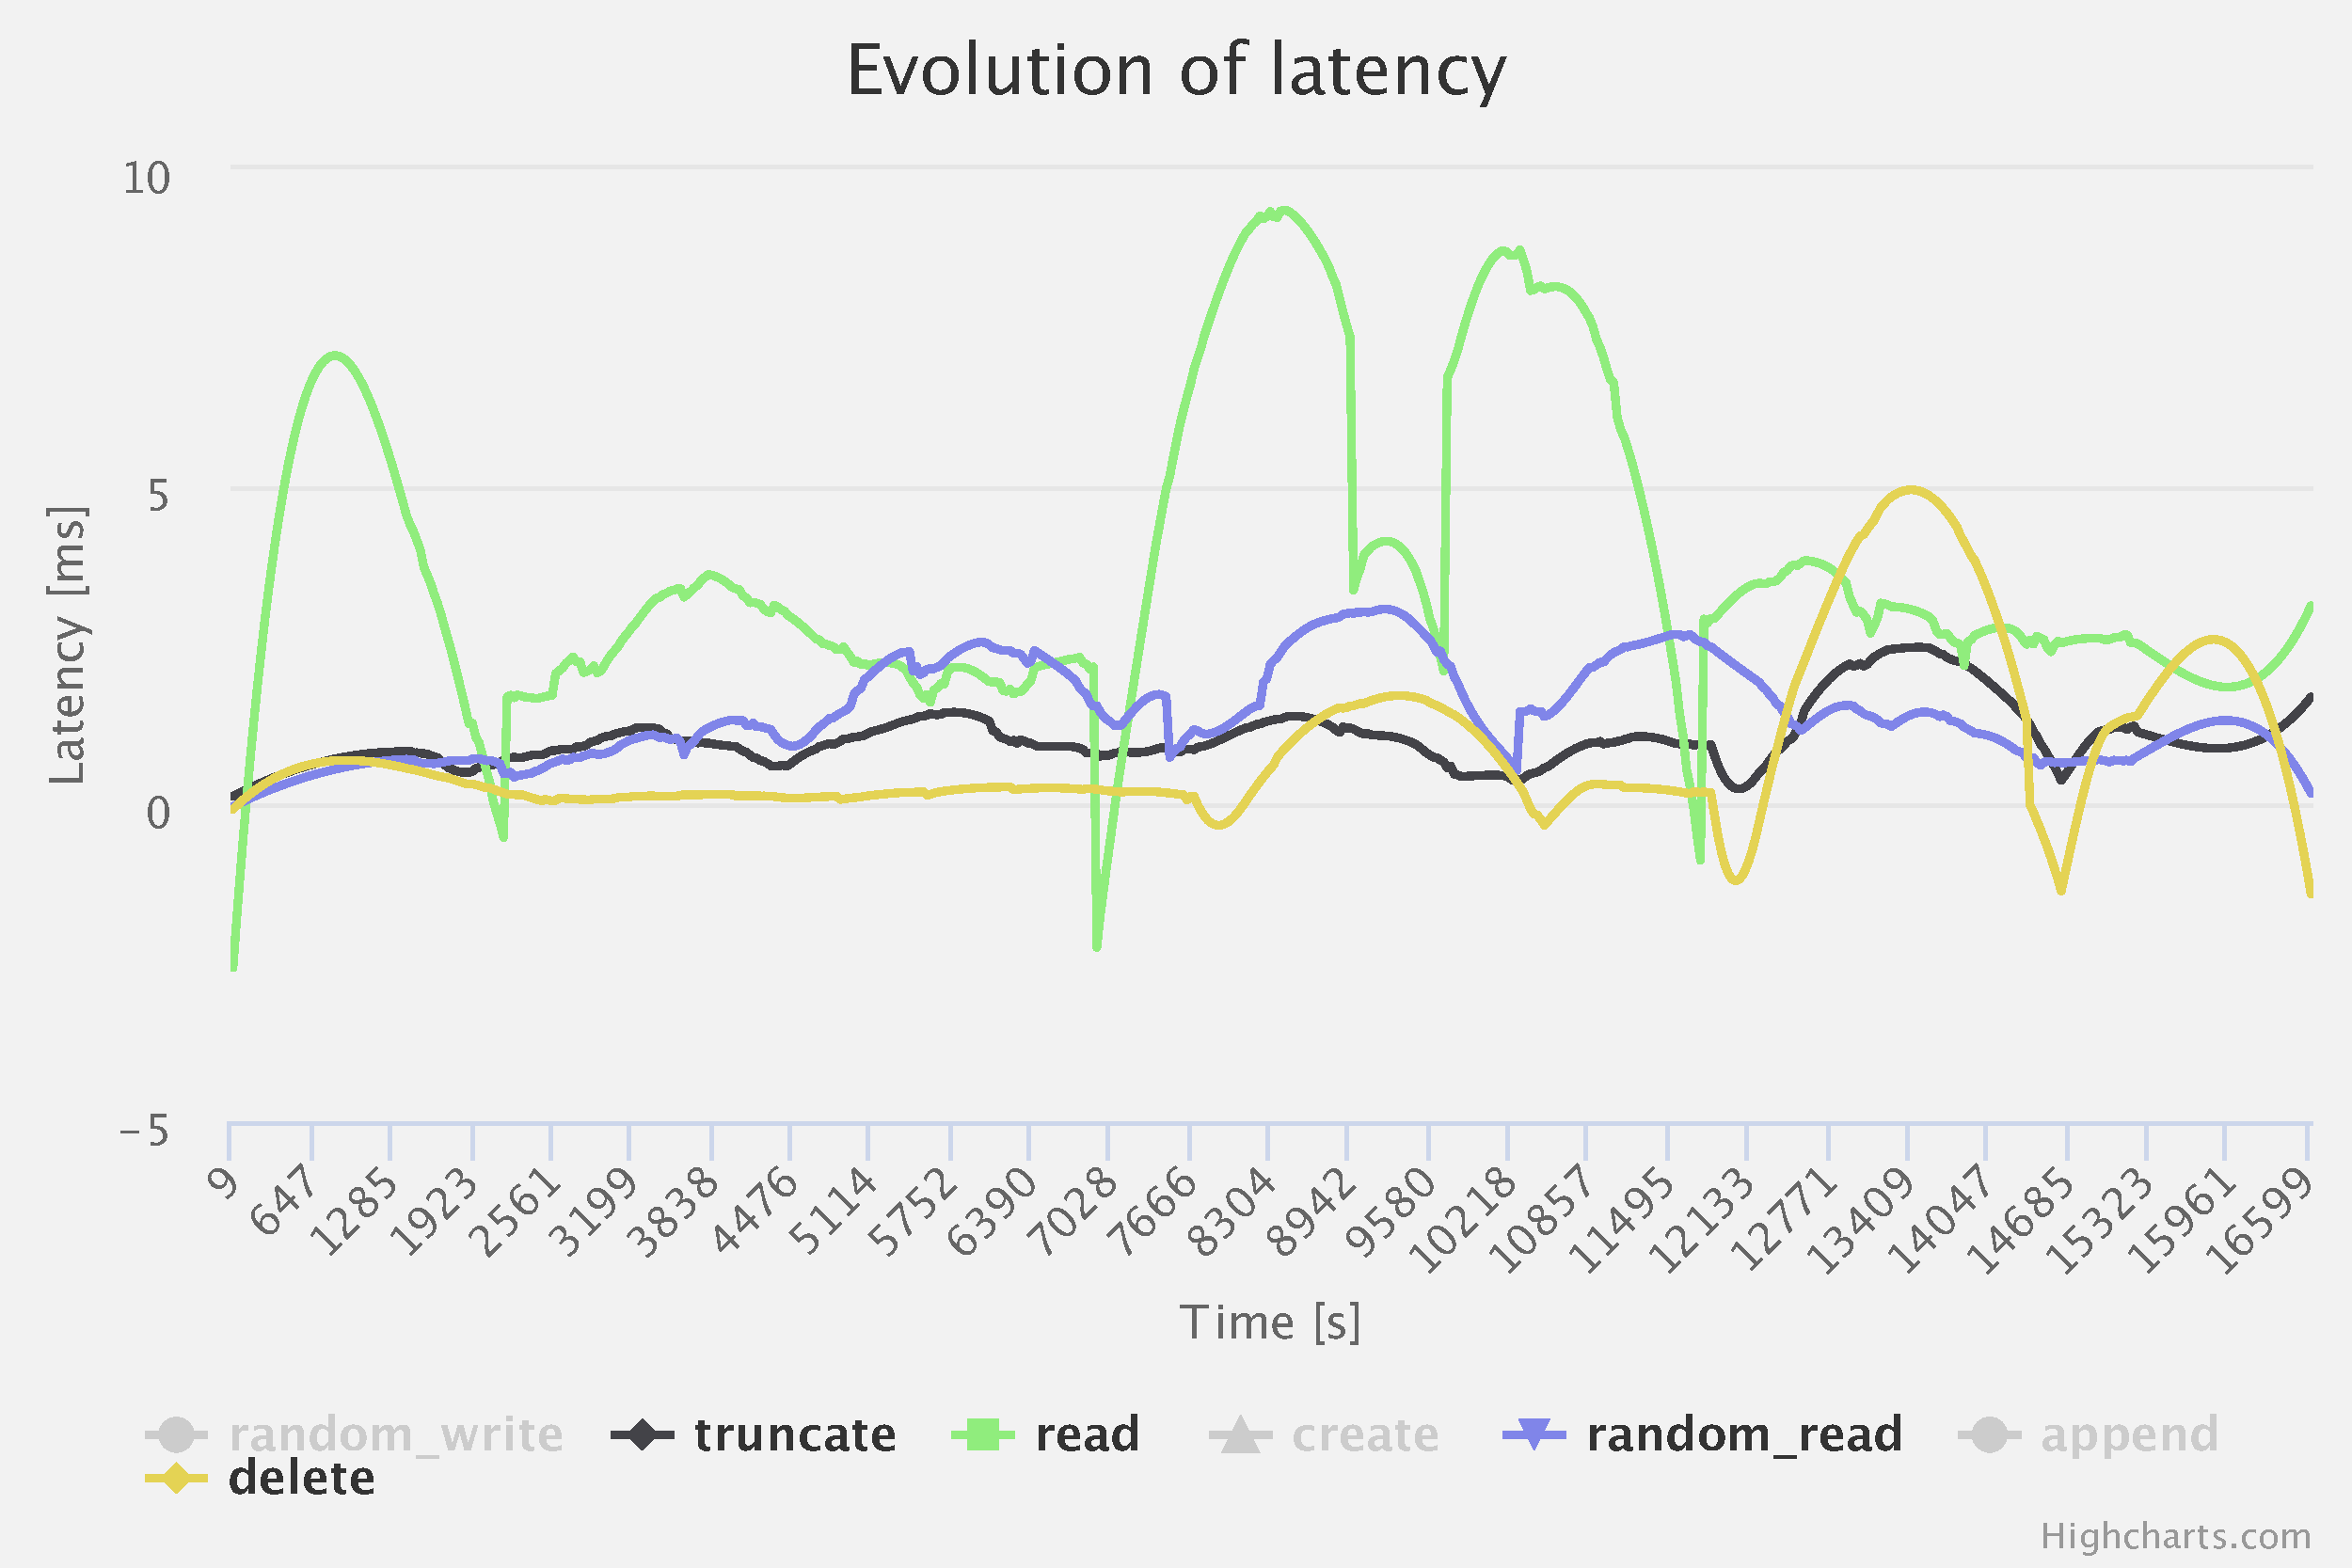
\includegraphics[width=\textwidth]{../charts/SSD_ext4_trim/1}
        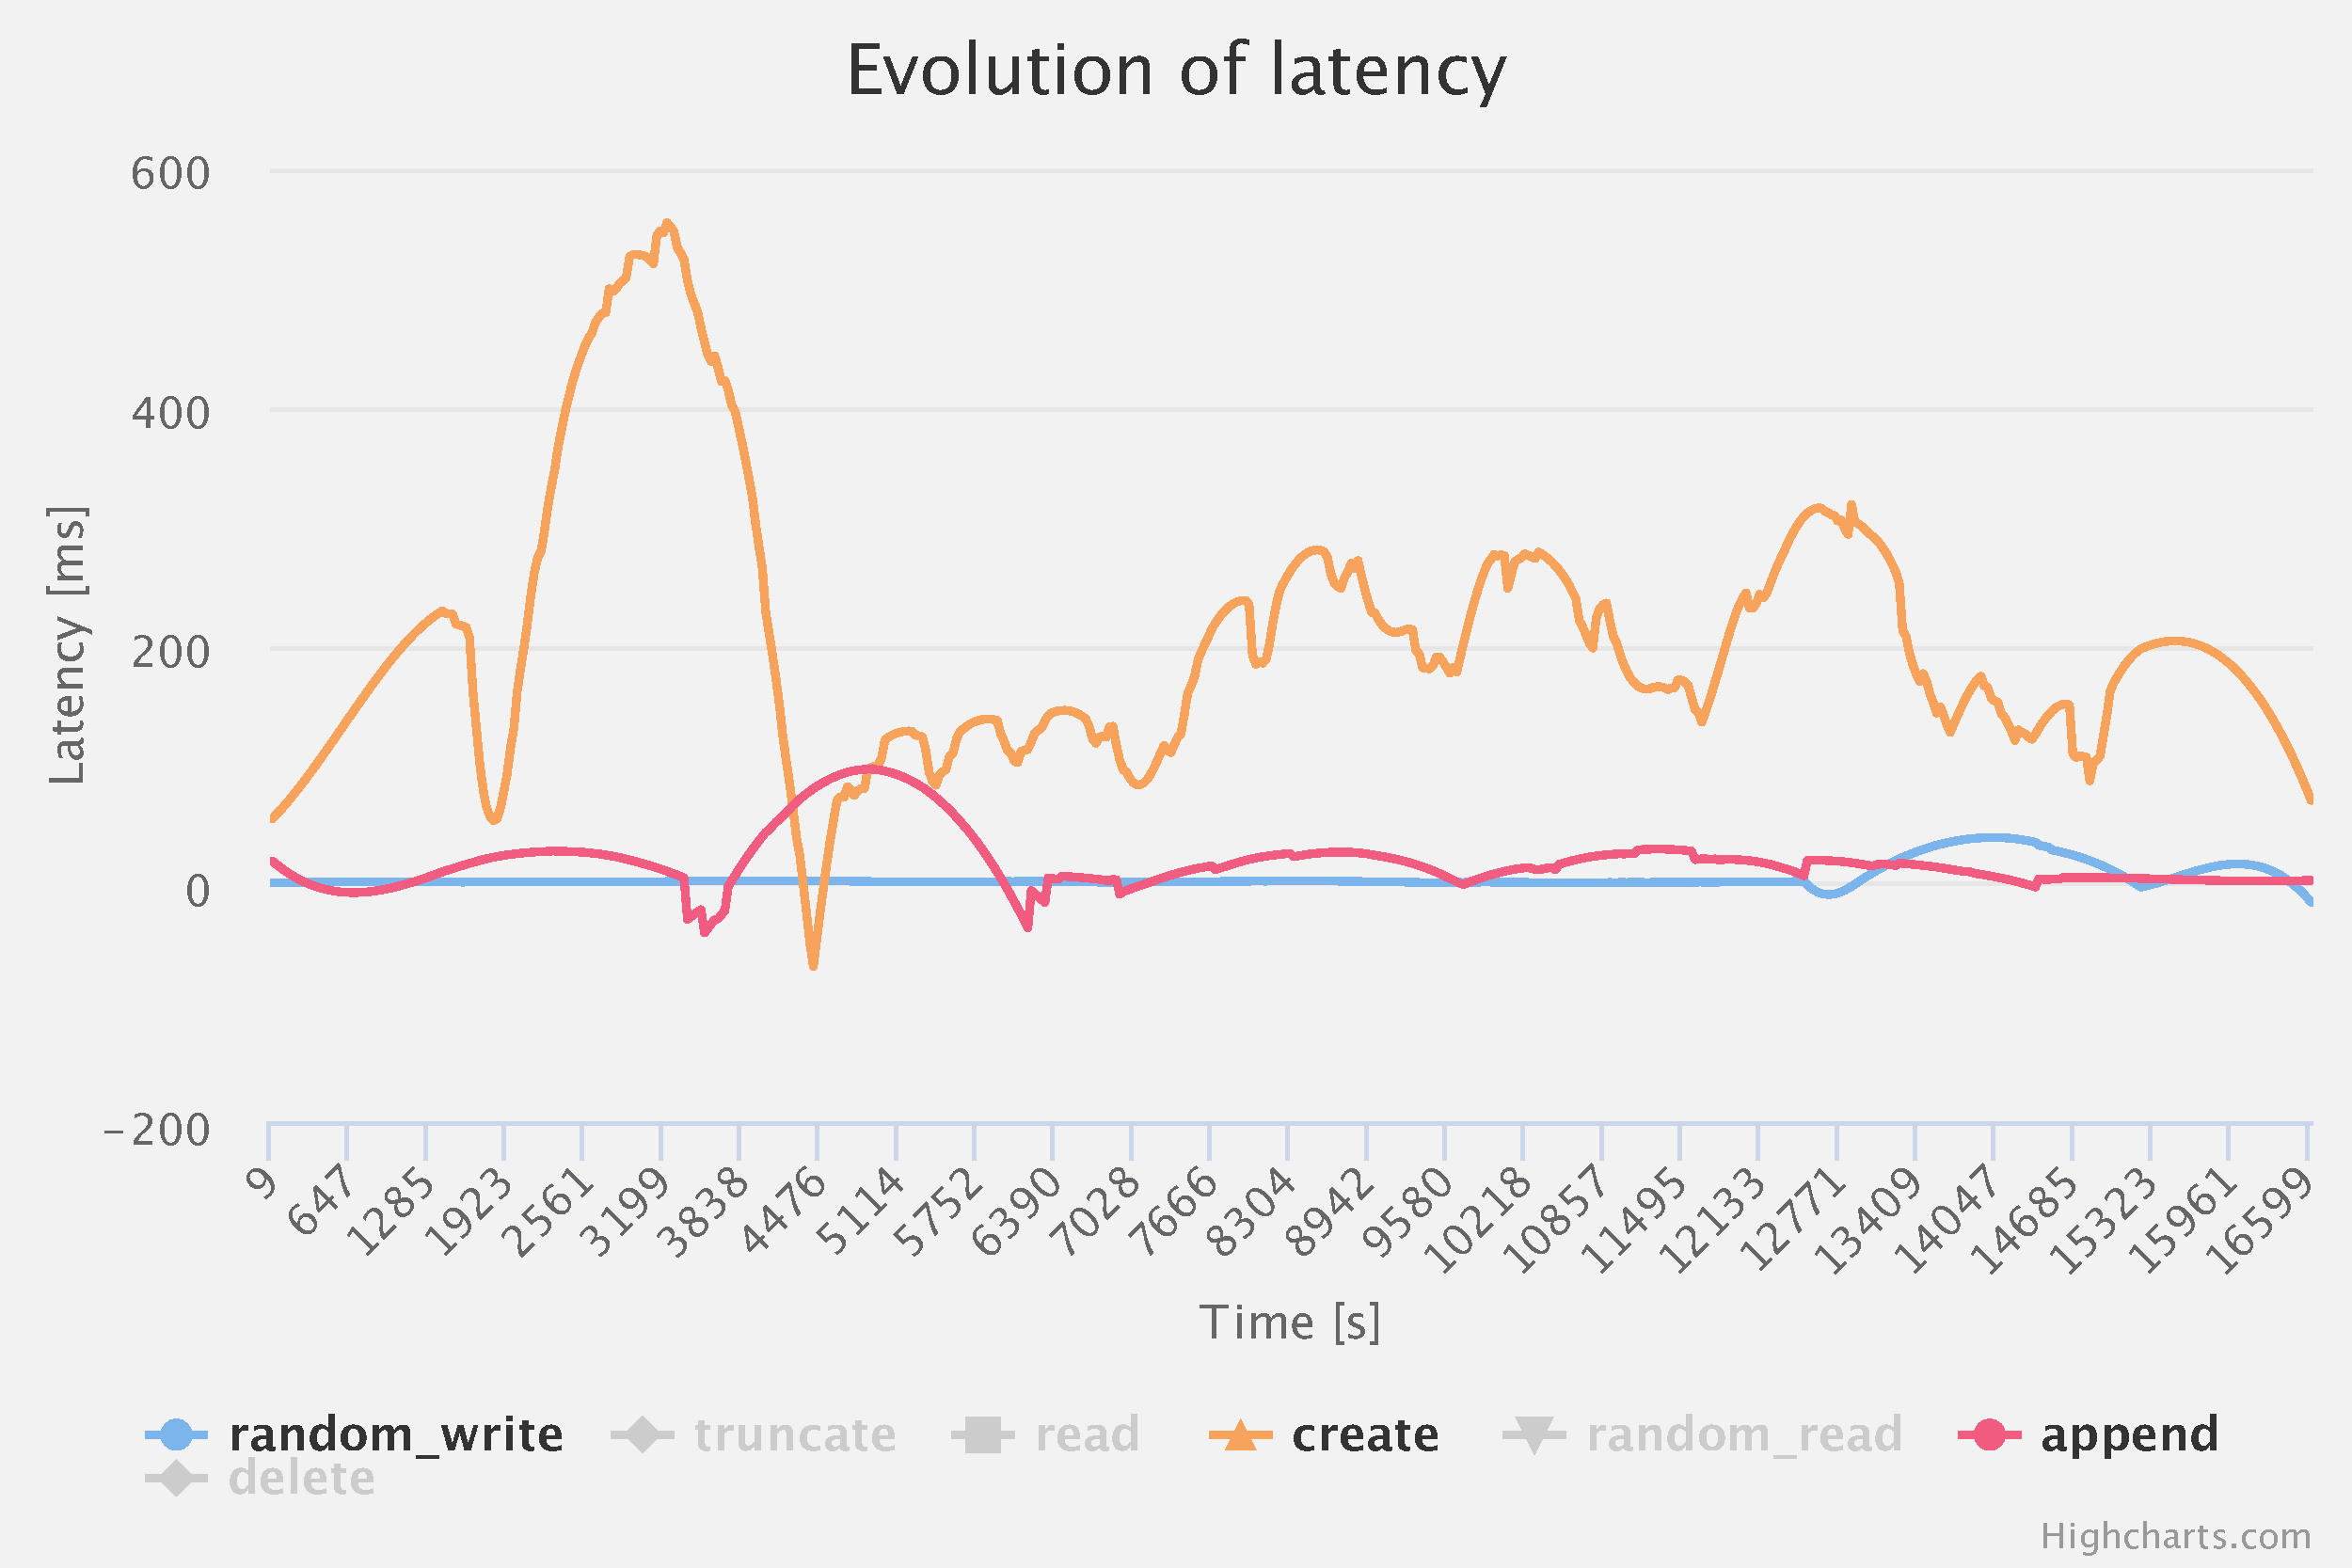
\includegraphics[width=\textwidth]{../charts/SSD_ext4_trim/2}
                \caption[Evolution of latencies of ext4 during testing on SSD with regular trimming]{Evolution of latencies of conducted IO operations during testing ext4 on SSD device with regular trimming performed. Some large fluctuations can be seen in sequential read operation, but otherwise not meaningful trend in change of performance van be observed.}
\label{fig:lats_ext4_ssd}
    \end{minipage}
\end{figure}

\clearpage


\section{Test of XFS on SSD without regular trimming}

\begin{itemize}
\itemsep0em 
   \item System: Machine\,2
   \item OS: RHEL-7.3
   \item Kernel: 3.10.0-514.el7.x86\_64
\end{itemize}

\begin{figure}[h]
    \centering
    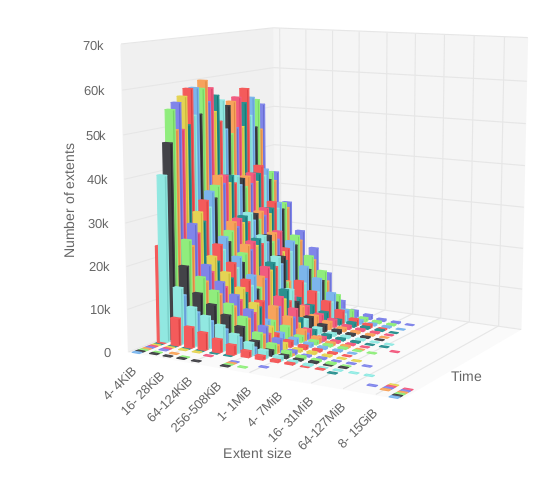
\includegraphics[width=\textwidth,keepaspectratio]{../charts/SSD_xfs_notrim/free.png}
    \caption[Evolution of free space fragmentation of XFS during testing on SSD without regular trimming]{This chart shows evolution of free space fragmentation through the whole test. When comparing this chart with Figure~\ref{fig:usage_ext4_ssd_trim}, we can see large raise of number of extents occurred after the test consumed all the available volume. We can see that untrimmed XFS file system has slightly more free space extents that trimmed XFS file system (Figure\ref{fig:free_xfs_ssd_trim})}
    \label{fig:free_xfs_ssd_notrim}
\end{figure}

\begin{figure}[h]
    \centering
    \fbox{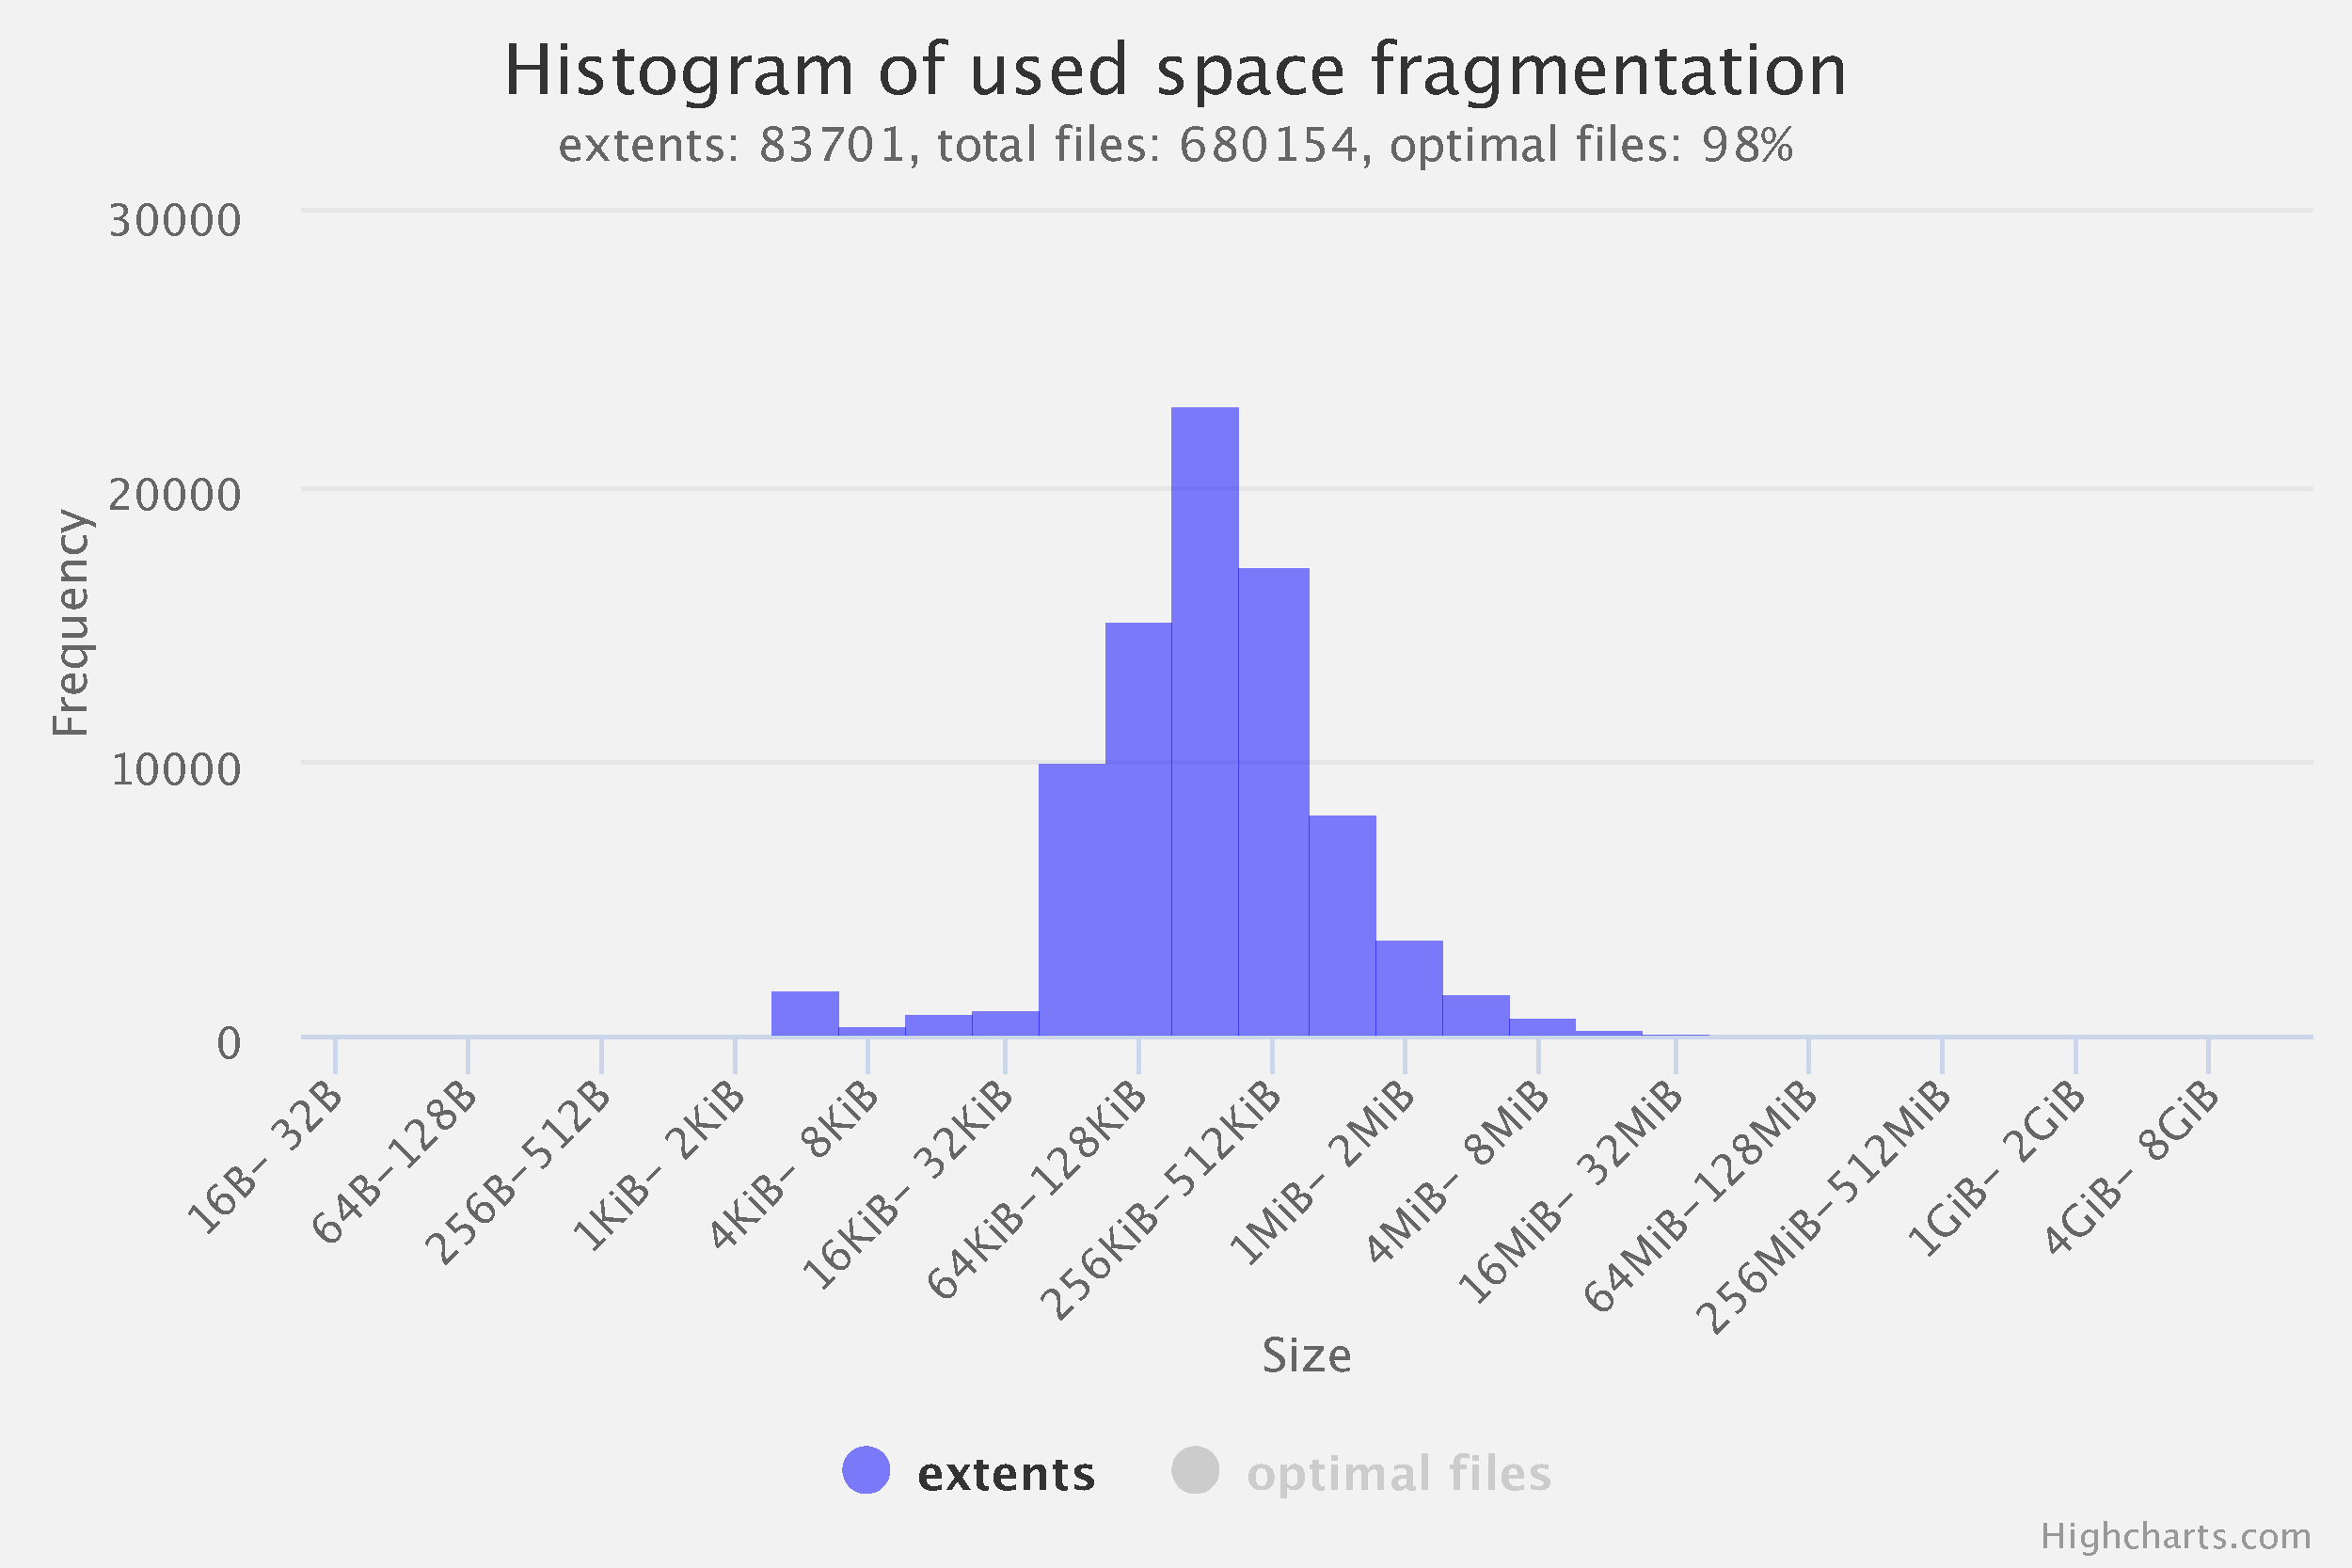
\includegraphics[width=\textwidth,keepaspectratio]{../charts/SSD_xfs_notrim/used}}
    \caption[Size distribution of file extents of XFS during testing on SSD without regular trimming]{On this chart, we can see distribution of size of file extents. Despite high fragmentation of free space during the test, the final block layout of file system have around 83 thousands of extents. 98\% of files were optimally allocated. Furthermore, we can observe that untrimmed XFS file system has more large file extents than trimmed. This can be caused by underlying device being slow, which in turn gives file system more time to reschedule its requests better.}
    \label{fig:used_xfs_ssd_notrim}
\end{figure}

\begin{figure}[!h]
    \begin{minipage}{\textwidth}
        \centering
        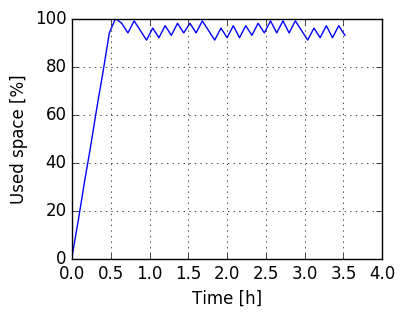
\includegraphics[width=0.7\textwidth]{../charts/SSD_xfs_notrim/usage.png}
        \caption[Usage of available space of XFS during testing on SSD without regular trimming]{Chart displays file system utilisation over time. Test filled the available volume ($\SI{120}{\giga\byte}$) in half an hour. Unless on trimmed tests, random file deleting iterations are observable on this graph, because the device was not able to fill volume in between data collecting intervals. This is a clear sign that untrimmed file system is significantly slower.}
\label{fig:usage_ext4_ssd_notrim}
\label{fig:usage_xfs_ssd_notrim}
    \end{minipage}
\end{figure}

\begin{figure}[!htb]
    \centering
   \begin{minipage}{\textwidth}
        \centering
        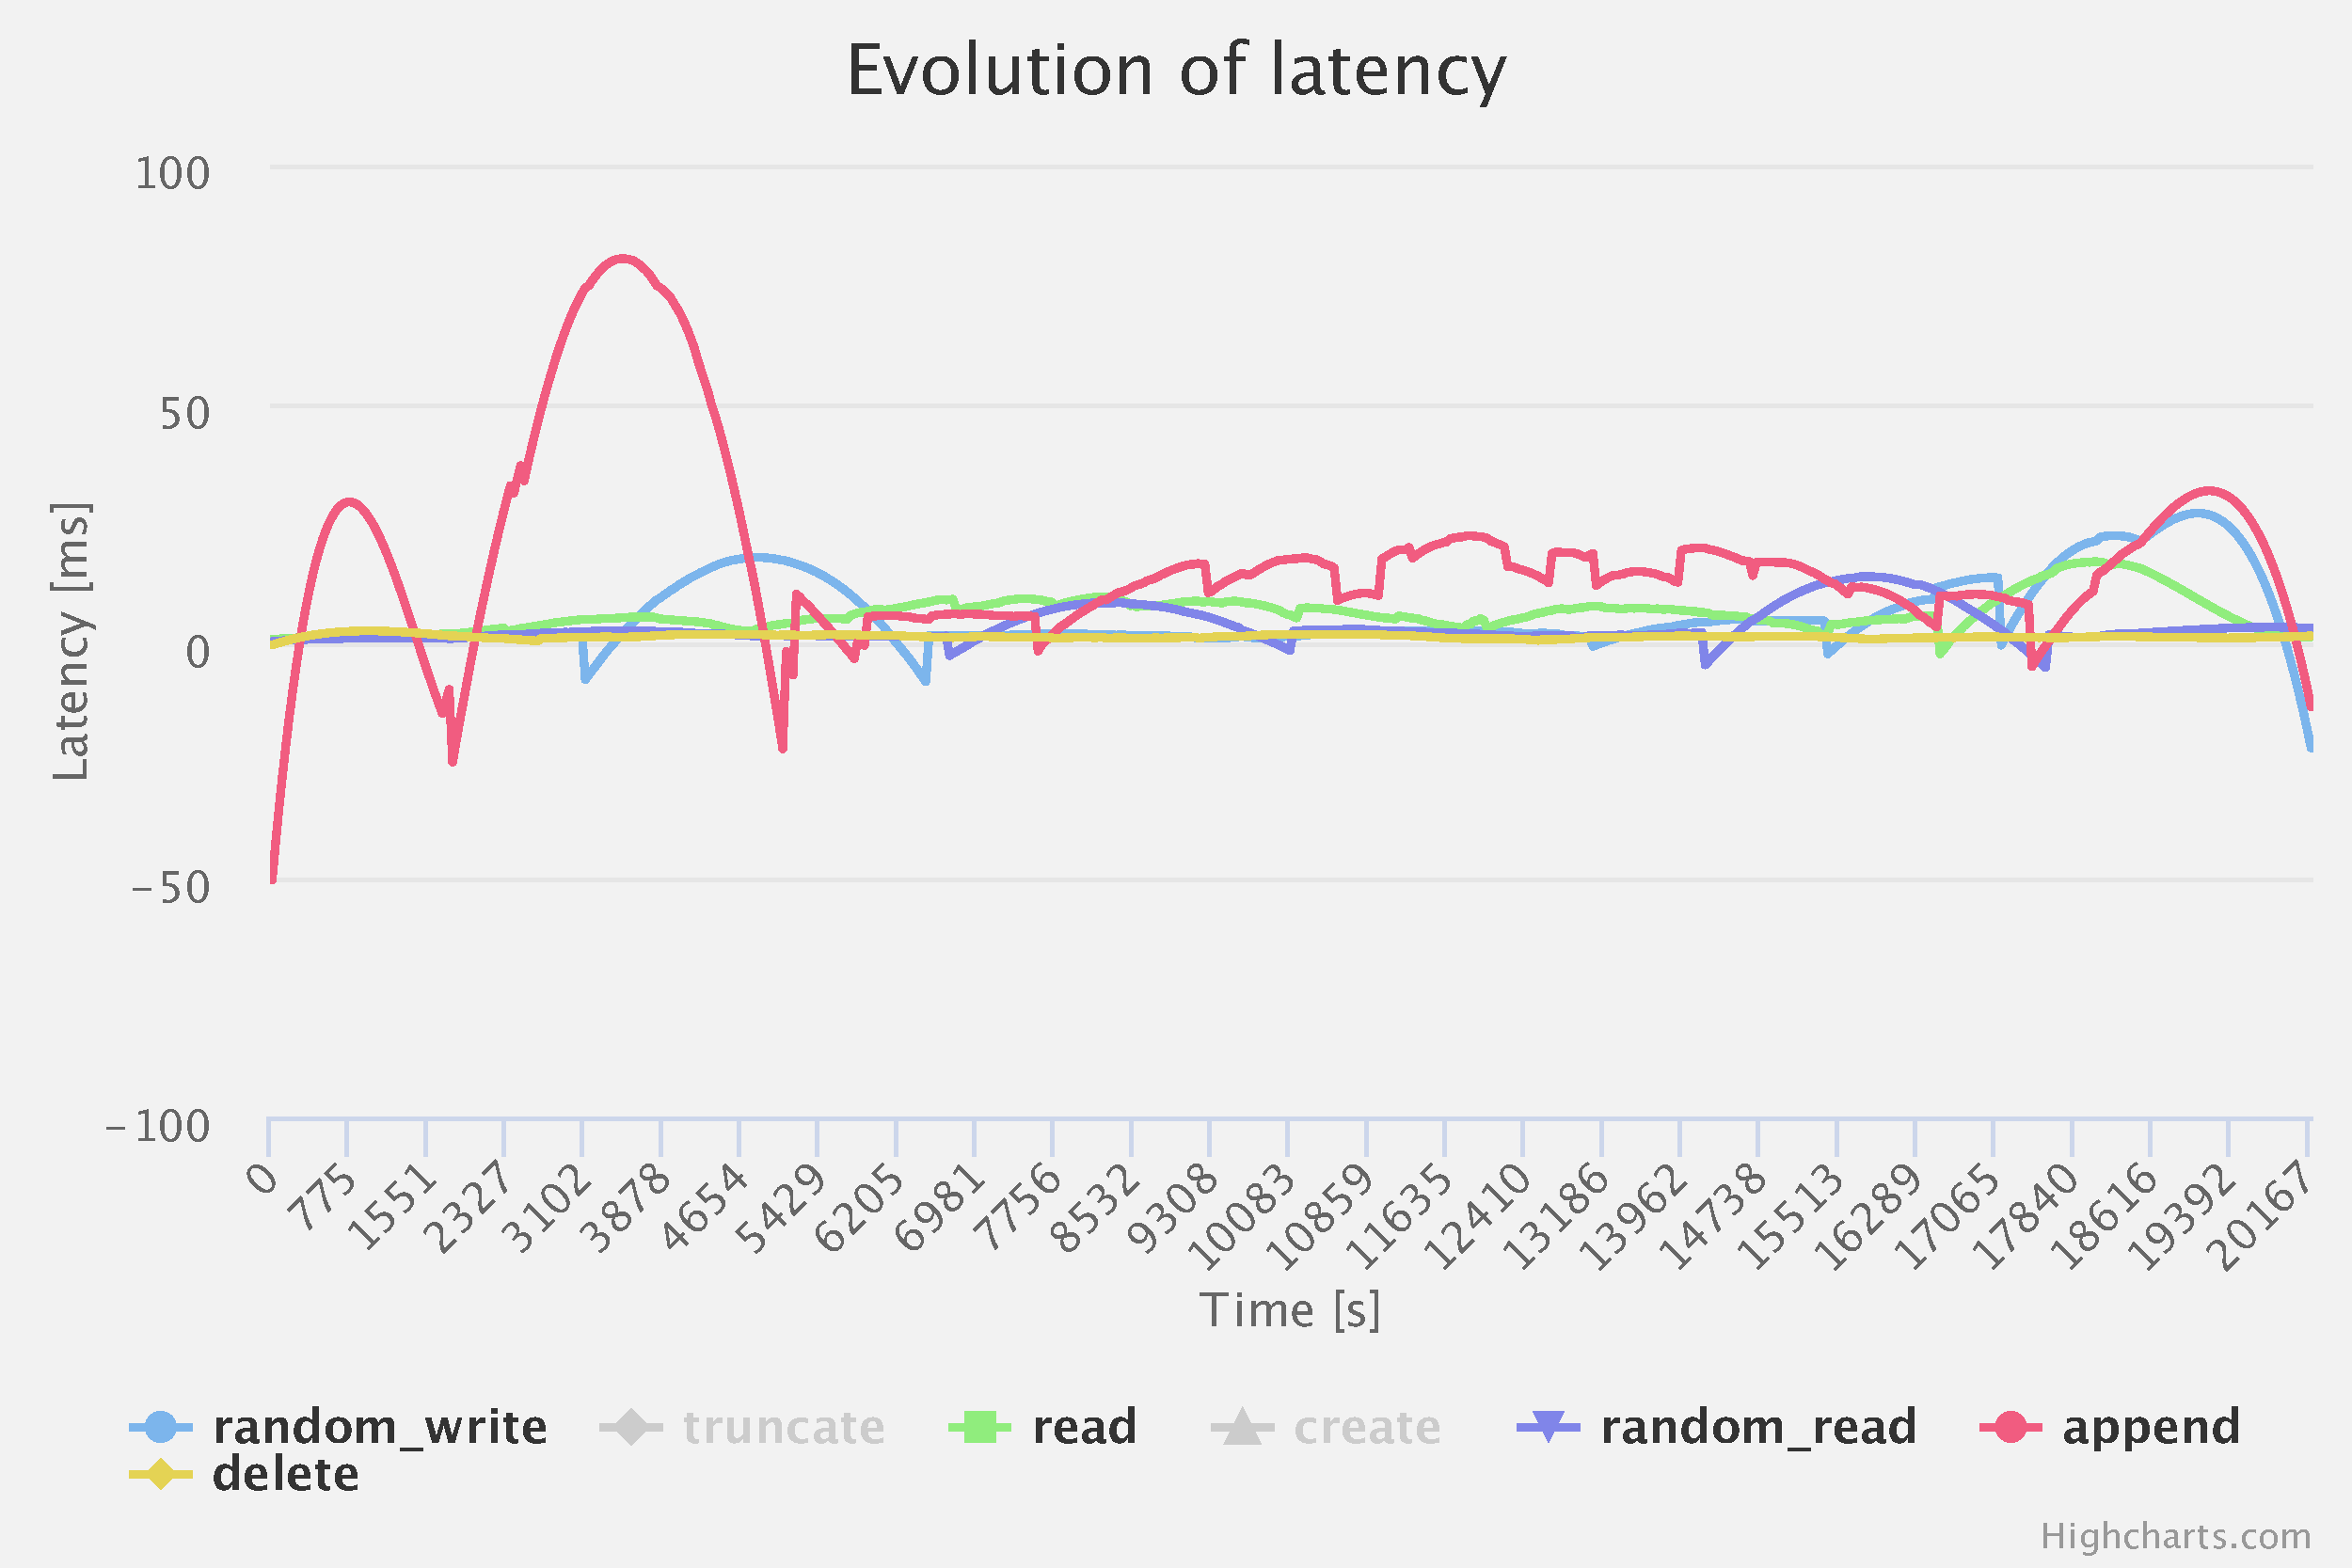
\includegraphics[width=\textwidth]{../charts/SSD_xfs_notrim/1}
        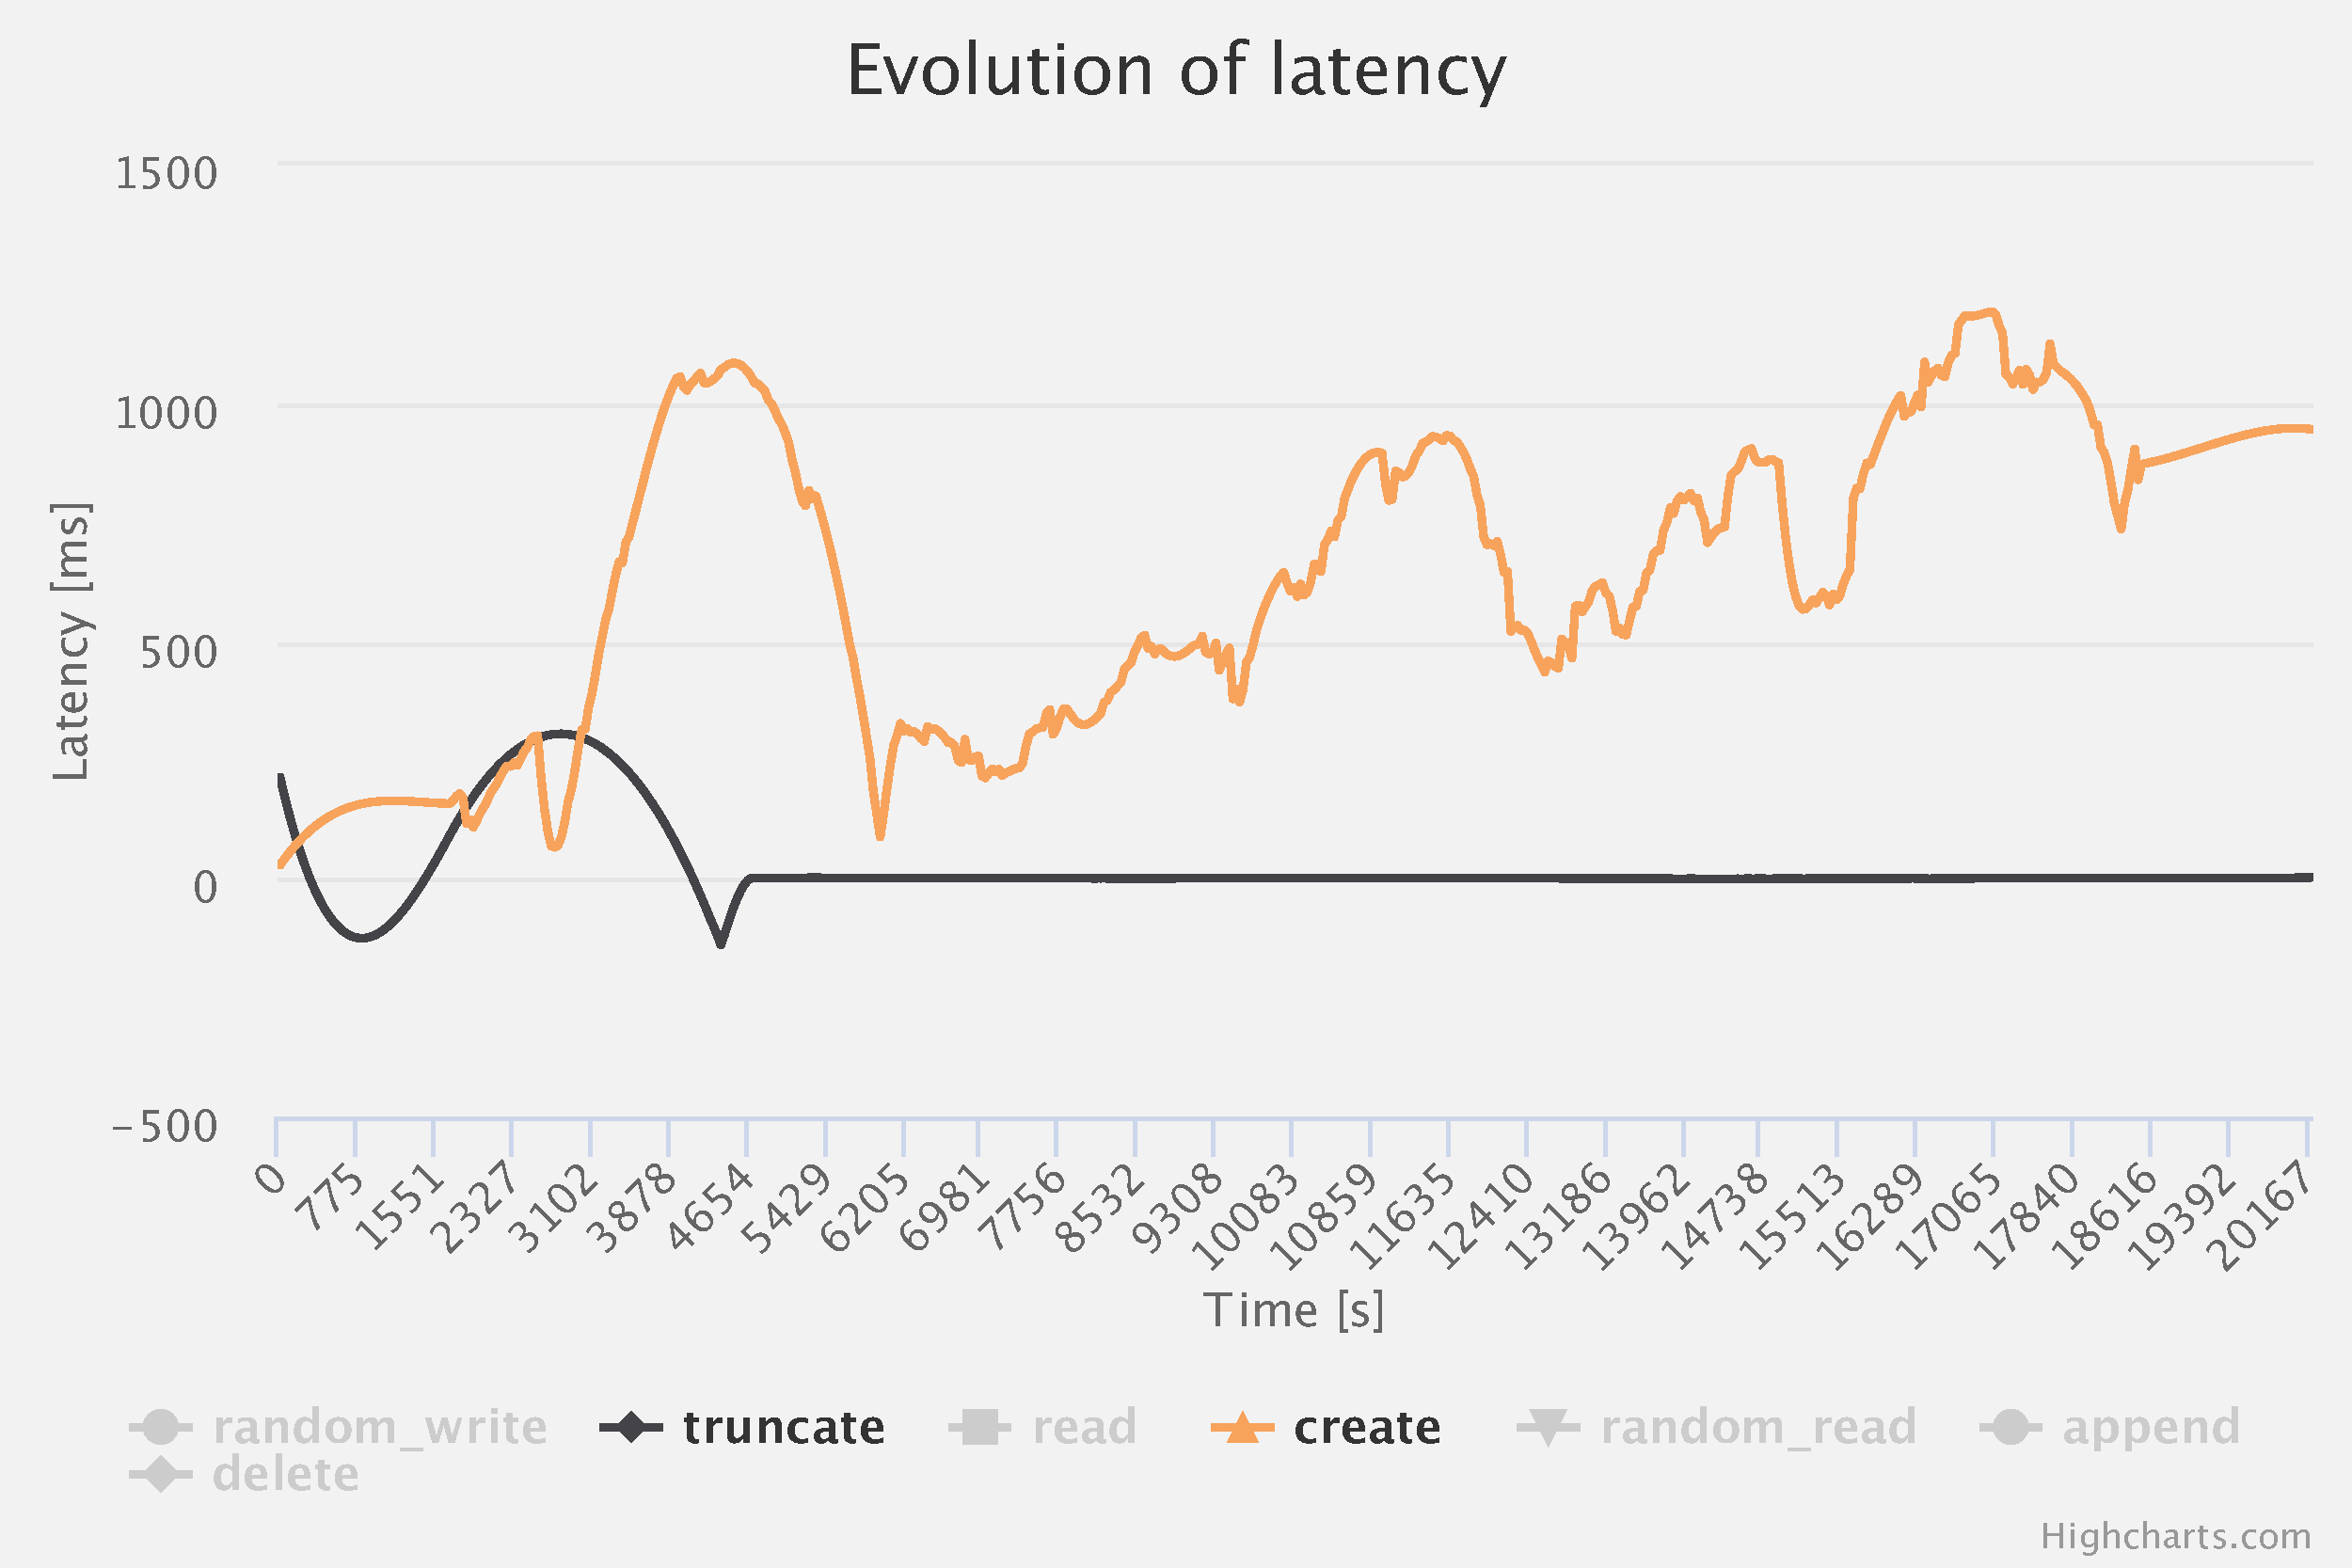
\includegraphics[width=\textwidth]{../charts/SSD_xfs_notrim/2}
                \caption[Evolution of latencies of XFS during testing on SSD without regular trimming]{Evolution of latencies of conducted IO operations during testing XFS on SSD device without regular trimming performed. Progressive degradation can be observed in create operation. There may be small growth and progressive larger fluctuations in sequential read, random read and random write.}
\label{fig:lats_xfs_ssd_notrim}
    \end{minipage}
\end{figure}

\clearpage

\chapter{Examples}
\label{examples}
\lstset{language=XML, 
numbers=left, 
frame=single, 
commentstyle=\color{dkgreen}, 
basicstyle={\scriptsize\ttfamily}, 
keywordstyle=\color{blue}, 
%identifierstyle=\color{blue}, 
stringstyle=\color{red},
captionpos=t,
showstringspaces=false,
breaklines=true,
breakatwhitespace=false,
tabsize=3,
caption={},
}


\begin{lstlisting}[language=xml, caption={Specifying OS to be installed in Beaker environment}, label={ex:os}][frame=single]
<distroRequires>
  <and>
    <distro_family op="=" value="RedHatEnterpriseLinux7"/>
    <distro_variant op="=" value="Server"/>
    <distro_name op="=" value="RHEL-7.3"/>
    <distro_arch op="=" value="x86_64"/>
  </and>
</distroRequires>
\end{lstlisting}


\begin{lstlisting}[language=xml, caption={Configuring environment and installing packages using kickstart}, label={ex:kickstart}][frame=single]
<kickstart>
<![CDATA[

install
lang en_US.UTF-8
skipx
keyboard us
rootpw redhat 
firewall --disabled
authconfig --enableshadow --enablemd5
selinux --enforcing
timezone --utc Europe/Prague

bootloader --location=mbr --driveorder=sda
zerombr
clearpart --all --initlabel --drives=sda
part /boot --fstype=ext2 --size=200 --asprimary --label=BOOT --ondisk=sda
part /mnt/tests --fstype=ext4 --size=40960 --asprimary --label=MNT --ondisk=sda
part / --fstype=ext4 --size=1 --grow --asprimary --label=ROOT  --ondisk=sda
reboot
%packages --excludedocs --ignoremissing --nobase
@core
wget
python
perl-devel
parted
cpuspeed
perl
dhcpv6-client
dhclient
yum
yum-rhn-plugin
yum-security
yum-updatesd
openssh-server
openssh-clients
bc
screen
nfs-utils
seekwatcher
sysstat
xfsprogs
e2fsprogs
hdparm
sdparm
gcc
tuned
cpufrequtils
cryptsetup-luks
vim-enhanced
rsync
lvm2
smartmontools
git
iotop
%end			
]]>
</kickstart>
\end{lstlisting}


\begin{lstlisting}[language=xml, caption={Configuring single device and file system ext4 using storage generator},label={ex:storage_generator}][frame=single]
      <task name="/kernel_fsperf/storage_generator" role="STANDALONE">
        <params>
          <param name="TEST_PARAM_STORAGE_GENERATOR" value="-s create -f ext4 -t single -m /RHTSspareLUN1 -d /dev/sdc -T 1SASHDD_ext4"/>
        </params>
      </task>
\end{lstlisting}
\begin{lstlisting}[language=xml, caption={Scheduling performance test of aged file system in Beaker environment},label={ex:fio}][frame=single]
      <task name="/kernel_fsperf/recipe_fio_aging" role="STANDALONE">
        <params>
          <param name="TEST_PARAM_RECIPE_FIO" value="-s 1 -r rw=randwrite-bs=4k-runtime=10m-fsync=64-direct=1-ioengine=libaio-thread-group_reporting-numjobs=10-size=1g-time_based-nrfiles=2441-openfiles=100-create_on_open=1 -D /dev/sdb1 -f ext4 -d 0 -t 1SATASSD -q W495TRIM -n 3"/>
        </params>
      </task>
\end{lstlisting}
\clearpage
\begin{lstlisting}[language=xml, caption={Scheduling file system aging task in Beaker environment},label={ex:age}][frame=single]
      <task name="/performance/drift_job" role="STANDALONE">
        <params>
          <param name="TEST_PARAM_DRIFT_JOB" value="-s 1 -r -t_/RHTSspareLUN1-o_12000000-f_4000000-+v_10000-w_wtable4.csv-i_300-+D_gaussian-T_on-Y_50-N_on -d /dev/sdb1 -M /RHTSspareLUN1 -t 1SASHDD -q W4595 -m 5_99 -f 0"/>
        </params>
      </task>
\end{lstlisting}

\chapter{Source code}
\label{source}
Source code of implemented tests, data processing tools and generated reports can be found in archive Appendix.tar.xz. The archive contains following directories:

\begin{itemize}
\itemsep0em 
   \item drift\_job: Contains implementation of automated aging test workflow.
   \item recipe\_fio\_aging: Contains implementation of automated performance testing workflow of aged file systems.
   \item data\_processing: Contains tools for automated data processing
   \item fs-drift: Contains used version of fs-drift.
   \item reports: Contains generated reports with interactive charts.
\end{itemize}



\end{document}
